% arara: makeindex

% Template for IEEE papers
%% bare_conf.tex
%% V1.4b
%% 2015/08/26
%% by Michael Shell
%% See:
%% http://www.michaelshell.org/
%% for current contact information.
%%
%% This is a skeleton file demonstrating the use of IEEEtran.cls
%% (requires IEEEtran.cls version 1.8b or later) with an IEEE
%% conference paper.
%%
%% Support sites:
%% http://www.michaelshell.org/tex/ieeetran/
%% http://www.ctan.org/pkg/ieeetran
%% and
%% http://www.ieee.org/

%%*************************************************************************
%% Legal Notice:
%% This code is offered as-is without any warranty either expressed or
%% implied; without even the implied warranty of MERCHANTABILITY or
%% FITNESS FOR A PARTICULAR PURPOSE!
%% User assumes all risk.
%% In no event shall the IEEE or any contributor to this code be liable for
%% any damages or losses, including, but not limited to, incidental,
%% consequential, or any other damages, resulting from the use or misuse
%% of any information contained here.
%%
%% All comments are the opinions of their respective authors and are not
%% necessarily endorsed by the IEEE.
%%
%% This work is distributed under the LaTeX Project Public License (LPPL)
%% ( http://www.latex-project.org/ ) version 1.3, and may be freely used,
%% distributed and modified. A copy of the LPPL, version 1.3, is included
%% in the base LaTeX documentation of all distributions of LaTeX released
%% 2003/12/01 or later.
%% Retain all contribution notices and credits.
%% ** Modified files should be clearly indicated as such, including  **
%% ** renaming them and changing author support contact information. **
%%*************************************************************************


% *** Authors should verify (and, if needed, correct) their LaTeX system  ***
% *** with the testflow diagnostic prior to trusting their LaTeX platform ***
% *** with production work. The IEEE's font choices and paper sizes can   ***
% *** trigger bugs that do not appear when using other class files.       ***                          ***
% The testflow support page is at:
% http://www.michaelshell.org/tex/testflow/

\documentclass{book}
\usepackage[quiet]{fontspec}
\usepackage[table,xcdraw,dvipsnames]{xcolor} % Used by spritegrid and others.
\usepackage[obeyspaces,spaces]{url}
\usepackage{longtable}
\usepackage{arydshln}
\usepackage{booktabs}
\usepackage{afterpage}
\usepackage{flushend}
\usepackage{titletoc}
\usepackage[toc]{appendix}
\usepackage{parskip}
\usepackage{graphicx,wrapfig}
\usepackage{float}
\usepackage{caption}
\usepackage{pdfpages}
\usepackage{tikzpagenodes}
\usepackage{imakeidx}
\usepackage[pagestyles,raggedright]{titlesec}
\usepackage[all]{nowidow}
\usepackage[bookmarks=true]{hyperref}
\usepackage{aeb-minitoc}
\usepackage{fix-cm}
\usepackage{textpos}
\usepackage{enumitem}
\usepackage{tcolorbox}
\tcbuselibrary{breakable,listings,skins,xparse}
%\usepackage{wrapfig}
\usepackage{needspace}
\usepackage{verbatim}
\usepackage{ean13isbn}
\usepackage{setspace}

% Use CHAPTER-PAGE page numbering to make it easier to modify chapters
% later, without messing up page number of the rest of the book.
\usepackage[auto]{chappg}

% Allow cross-references between the various books to the big The MEGA65 Book
\usepackage{xr}
\usepackage{varioref}
\usepackage{xparse}
\externaldocument[M65Book-]{mega65-book}
% And a \ref alternative that checks if it needs to be a cross-reference to the
% MEGA65 Book instead.
\makeatletter
\newcommand{\bookref}[1]{%
    \@ifundefined{r@#1}{%
      {\em the MEGA65 Book}, \nameref{M65Book-#1} (\autoref{M65Book-#1})}{\autoref{#1}}%
}
\newcommand{\bookvref}[1]{%
    \@ifundefined{r@#1}{%
      {\em the MEGA65 Book}, \nameref{M65Book-#1} (\autoref{M65Book-#1})}{Chapter/Appendix \vref{#1}}%
}
\makeatother

% For fixed-width columns in register maps
\usepackage{array}

% Makes tables with double-ruled lines look better
\usepackage{hhline}

% Makes better use of space for reference tables in appendix
\usepackage{multicol}

% Shaded tables with alternate rows colored for better legibility
% Best used with larger tables rather than small tables
\usepackage{colortbl}
\usepackage{adjustbox}
\usepackage[strict]{changepage}

% \makecell command for forcing line breaks in table cells
\usepackage{makecell}

\newcolumntype{L}[1]{>{\raggedright\let\newline\\\arraybackslash\hspace{0pt}}m{#1}}
\newcolumntype{C}[1]{>{\centering\let\newline\\\arraybackslash\hspace{0pt}}m{#1}}
\newcolumntype{R}[1]{>{\raggedleft\let\newline\\\arraybackslash\hspace{0pt}}m{#1}}

% For displaying Letter keys and the MEGA key
% This is a `keys' element for displaying a Mega65 keyboard key
% using a black filled label with rounded edges.
% In order to display a key as a title, use:
%
%     \megakey[title]{Run/Stop}
%
% For displaying a key as a part of the normal document flow, simply use:
%
%    \specialkey{SHIFT}
%
%
% If you get warnings on special characters, mathematical characters etc, use $, eg:
%
%    \megakey{$\leftarrow$}
%
% Other sizes are supported, as part of tcolorbox:
% http://mirror.aarnet.edu.au/pub/CTAN/macros/latex/contrib/tcolorbox/tcolorbox.pdf#subsubsection.4.7.5 however, only `title' and the default: `small' are proposed for use in this manual.
%
% The second macro available here is the megasymbolkey.
% This will display the MEGA symbol as white on a black key box. Simply use:
%
%		 \megasymbolkey
%
% Some MEGA65 keys contain two lines of text like "RUN/STOP"
% You can use the specialkey macro for this:
%
%    \specialkey{SHIFT LOCK}%

\usepackage{tcolorbox}

\newtcbox{\megakeyinner}[1][small]{colback=black, coltext=white, size=#1, fontupper=\bfseries, nobeforeafter,box align=bottom,baseline=3pt,text height=7pt}
\newcommand{\megakey}[2][small]{\megakeyinner[#1]{\uppercase{#2}}}

% Previous version of megasymbolkey
%\newtcbox{\megasymbolkeyinner}{colback=black, coltext=white, clip title=false. fontupper=\symbolfont, box align=bottom,baseline=3pt,text height=7pt}
%\newcommand{\megasymbolkey}{\megakeyinner{\megasymbol[white]}\ }

\newtcolorbox{megasymbolkeyinner}
{colback=black,coltext=white,size=small,fontupper=\small\bfseries,
width=0.65cm, height=0.55cm, box align=base,
nobeforeafter, halign=flush left, left=0mm,top=0.3mm,bottom=0mm,right=0mm
,boxsep=0.5mm,baseline=4pt, enlarge right by = 1mm
}
\newcommand{\megasymbolkey}{
\begin{megasymbolkeyinner}%
\megasymbol[white]%
\end{megasymbolkeyinner}%
}

\newtcolorbox{specialkeyinner}
{colback=black,coltext=white,size=small,fontupper=\tiny\bfseries,
width=0.80cm, height=0.55cm, box align=base,
nobeforeafter, halign=flush left, left=0mm,top=0.3mm,bottom=0mm,right=0mm
,boxsep=0.5mm,baseline=4pt
}
\newcommand{\specialkey}[1]{
\begin{specialkeyinner}%
#1%
\end{specialkeyinner}%
}

\newtcolorbox{widekeyinner}
{colback=black,coltext=white,size=small,fontupper=\tiny\bfseries,
width=0.9cm, height=0.55cm, box align=base,
nobeforeafter, halign=flush left, left=0mm,top=0.3mm,bottom=0mm,right=0mm
,boxsep=0.5mm,baseline=4pt
}
\newcommand{\widekey}[1]{
\begin{widekeyinner}%
#1%
\end{widekeyinner}%
}




% For displaying print versions petscii character symbols
% This is a collection of symbol macros element for displaying a printed version of the
% MEGA65 graphic characters, as opposed to the bitmap versions in the mega40/80.ttf fonts files.
% You can display characters using the graphicsymbol macro:
%
%    \graphicsymbol{\textcolor{red}{qQ} wWUcbdhjI \textcolor{blue}{JK}}
%
% Or you can, simply use the font itself:
%
%    \begin{symbolfont}%
%	   qQwWeErRtTyYuUiIoOpP\\
%		 aAsSdDfFgGhHjJkKlL\\
%		 zZxXcCvVbBnNmM%
%		 \end{symbolfont}%
%
%
% You can display the MEGA symbol using:
%
%    \megasymbol
%
% This will display the symbol in black. Other colours can be specified by passing them in, for example:
%
% 	 \megasymbol[black]
%		 \megasymbol[white]
%		 \megasymbol[orange]
%		 \megasymbol[blue]
%
% NOTE:
% For using the MEGA symbol in a key, see the \megasymbolkey macro in the keys.txt file.

\usepackage{tcolorbox}

\newcommand{\graphicsymbol}[1]{\begin{symbolfont}#1\end{symbolfont}}

\newcommand{\megasymbol}[1][black]{\begin{symbolfont}\textcolor{#1}{`}\end{symbolfont}}


% For Mega65 display of code, listings and screen activity
\input{elements/screenoutput}

% For MEGA65 screen shots with text flow
\input{elements/screenshots}

% For displaying sprite data in a grid
% This is an element for displaying a sprite in a grid, just like page 70 of the
% commodore manual. This version can be easily expanded. For now it will suffice.
% In order to display a hi-res mono sprite grid use:
%
%	\spritegrid{
%	\hline
%	\spritecells{---------ooooo----------}
%	\spritecells{-------ooooooooo--------}
%	\spritecells{------ooooooooooo-------}
%	\spritecells{------ooo--o---oo-------}
%	\spritecells{-----ooo-ooo-ooooo------}
%	\spritecells{-----ooo-ooo-ooooo------}
%	\spritecells{-----ooo---o---ooo------}
%	\spritecells{-----ooo-o-ooo-ooo------}
%	\spritecells{-----ooo-o-ooo-ooo------}
%	\spritecells{-----ooo---o--oooo------}
%	\spritecells{------ooooooooooo-------}
%	\spritecells{------ooooooooooo-------}
%	\spritecells{-------ooooooooo--------}
%	\spritecells{-------o-ooooo-o--------}
%	\spritecells{--------o-o-o-o---------}
%	\spritecells{--------o--o--o---------}
%	\spritecells{---------o-o-o----------}
%	\spritecells{---------o-o-o----------}
%	\spritecells{---------ooooo----------}
%	\spritecells{---------ooooo----------}
%	\spritecells{----------ooo-----------}
%	}
%
% For a multicolour sprite:
%
%	\spritegrid{
%	\hline
%	\spritecells{------------------------}
%	\spritecells{------------------------}
%	\spritecells{------------------------}
%	\spritecells{------------------------}
%	\spritecells{llllllllllllllllllllllll}
%	\spritecells{llllllllllllllllllllllll}
%	\spritecells{lllllleeeeeelleeeeeeeell}
%	\spritecells{lllloooooooollooooooooll}
%	\spritecells{llllooggggggllooggggggll}
%	\spritecells{lllloolllllllloollllllll}
%	\spritecells{llllooeeeellllooeeeellll}
%	\spritecells{lllloooooooollooooooooll}
%	\spritecells{llllooggggoollggggggooll}
%	\spritecells{lllloolllloollllllllooll}
%	\spritecells{llllooeeeeoolleeeeeeooll}
%	\spritecells{llllggooooggllooooooggll}
%	\spritecells{llllllggggllllggggggllll}
%	\spritecells{llllllllllllllllllllllll}
%	\spritecells{------------------------}
%	\spritecells{------------------------}
%	\spritecells{------------------------}
%	}

\usepackage{tabulary} %Removes spacing from tabulars
\usepackage{xstring} % for string substitution
\usepackage{xparse} % used for unpacking the sprite characters
% \renewcommand{\familydefault}{\sfdefault} % default sans font

%\usepackage{graphicx} % for resizing the tabular used by spritegrid
\usepackage{subcaption} % used for the left hand subtable of row numbers
\usepackage{multirow} % used for the ``Row'' column
\usepackage{rotating} % used by the rotating ``Row'' word

\newcommand{\spritebytecolumn}[1]{
   %\framebox[4mm]{#1}
   \makebox[4mm]{#1}
}

\setlength\tabcolsep{0.3mm} % the indivdual cell width and height


% Cell colour list. Can be expanded for other colours in the sprite grid
\def\blk{\cellcolor{black}}
\def\wht{\cellcolor{white}}
\def\grn{\cellcolor{ForestGreen}}
\def\lgrn{\cellcolor{YellowGreen}}
\def\gry{\cellcolor{Gray}}

\newcounter{lettercounter} % counter for detecting the last cell

% Collect the spritecell list and send it to \ProcessSpriteCell for turning into cells
\NewDocumentCommand{\spritecells}{%
>{\SplitList{}} m }{%
  \ProcessList{#1}{\ProcessSpriteCell}%
}

\NewDocumentCommand{\ProcessSpriteCell}{m}{%
  \stepcounter{lettercounter}%
    \IfStrEqCase{#1}{
	{o}{\blk}
	{-}{\wht}
	{g}{\grn}
	{l}{\lgrn}
	{e}{\gry}
   }%
   \IfStrEq{\thelettercounter}{24}{\setcounter{lettercounter}{0} \\ \hline}{&}%
}

% Start of the actual spritegrid definition
\newcommand{\spritegrid}[1]{
\begin{table}[h!]
\centering
\begin{subtable}{28mm}
\vspace{8mm}
\scalebox{0.76}{
\begin{center}
\begin{tabular}{p{25mm} p{4mm} c}
\multirow{21}{*}{ } &
\multirow{21}{*}{%
\begin{turn}{90}%
\bfseries\uppercase{Row}%
\end{turn}} &
 1\\
& & 2\\
& & 3\\
& & 4\\
& & 5\\
& & 6\\
& & 7\\
& & 8\\
& & 9\\
& & 10\\
& & 11\\
& & 12\\
& & 13\\
& & 14\\
& & 15\\
& & 16\\
& & 17\\
& & 18\\
& & 19\\
& & 20\\
& & 21
\end{tabular}
\end{center}
}
\end{subtable}%
\begin{subtable}{.8\textwidth}

\setlength{\arrayrulewidth}{1pt}
\scalebox{0.7}{
\begin{center}
\begin{tabular}{  *{3}{p{30mm} }  }
  \center\uppercase{Series\\1} &
  \center\uppercase{Series\\2} &
  \center\uppercase{Series\\3}
\end{tabular}
\end{center}
}

\scalebox{0.7}{
\begin{center}
\begin{tabular}{p{5.8mm} *{11}{C{7.3mm}}}
   128 & 32 & 8 & 2 & 128 & 32 & 8 & 2 & 128 & 32 & 8 & 2
\end{tabular}
\end{center}
}
\\[-1.5mm]
\scalebox{0.7}{
\begin{center}
\begin{tabular}{p{1.7mm} *{12}{C{7.3mm}}}
  & 64 & 16 & 4 & 1 & 64 & 16 & 4 & 1 & 64 & 16 & 4 & 1
\end{tabular}
\end{center}
}

\scalebox{0.7}{
\begin{center}
\begin{tabular}{ | *{24}{p{3mm} |}  }
#1
\end{tabular}
\end{center}
}

\scalebox{0.7}{
\begin{center}
\begin{tabular}{ *{24}{p{3.35mm}}  }
	\spritebytecolumn{1} & & & &
	\spritebytecolumn{5} & & & & &
	\spritebytecolumn{10} & & & & &
	\spritebytecolumn{15} & & & & &
	\spritebytecolumn{20} & & & &
	\spritebytecolumn{24} \\
	\multicolumn{24}{c}{\bfseries\uppercase{Column}}
\end{tabular}
\end{center}
}
\end{subtable}
\end{table}
}

% End of the actual spritegrid definition



% Don't number sections
\setcounter{secnumdepth}{0}

\renewcommand{\indexname}{INDEX}
\renewcommand{\appendixtocname}{APPENDICES}
\renewcommand{\appendixpagename}{APPENDICES}
\renewcommand{\appendixpage}{%
  \clearpage\thispagestyle{empty}
    \pagecolor{blue}
     \begin{center}
       {
         \large
         % Put a nice amount of vertical space before the title
         \vspace*{2cm}
               {\large\Huge\textcolor{white}{\bf{APPENDICES}}}\\
             \vspace{\fill}
       }
     \end{center}
     \newpage\pagecolor{white}\clearpage
}

\makeatletter\chardef\pdf@shellescape=\@ne\makeatother

\setcounter{tocdepth}{5}

% 1.0 cm is the distance from left of page to bullet point.
% 2.8 cm is a fudge-factor to make multi-line section names be correctly lined up.
% \@B{〈length〉} is the amount to indent prior to〈sec-num >
% \@F{〈fmt〉} is the formatting for the title heading
% \@P{〈fmt〉} is the formatting for the page number (〈pg-num〉).

\TOCLevels{chapter}{section}
\begin{minitocfmt}{\chapmtoc}
\declaretocfmt{section}{\@F{\color{white}\hspace{1.0cm}\textbullet\hspace{0.25cm}\Large\bfseries}\@B{2.8cm}\@P{\mtocgobble}}
\declaretocfmt{section*}{\@F{\color{white}\hspace{1.0cm}\textbullet\hspace{0.25cm}\Large\bfseries}\@B{2.8cm}\@P{\mtocgobble}}
\end{minitocfmt}

\input{fonts}

% Set margins for inner and outer pages in A5 book format
\ifdefined\printmanual
\usepackage[a5paper,nomarginpar,includemp,bottom=2cm,top=1cm,inner=1.8cm,outer=0.8cm, footskip = 1cm]{geometry}
\else
\usepackage[a5paper,nomarginpar,includemp,bottom=2cm,top=1cm,inner=1.0cm,outer=1.0cm, footskip = 1cm]{geometry}
\fi

% Some Computer Society conferences also require the compsoc mode option,
% but others use the standard conference format.
%
% If IEEEtran.cls has not been installed into the LaTeX system files,
% manually specify the path to it like:
% \documentclass[conference]{../sty/IEEEtran}

%% \input{setup}

% correct bad hyphenation here
\hyphenation{op-tical net-works semi-conduc-tor}

\makeindex[intoc]

\pagestyle{empty}

\begin{document}
\raggedbottom

% relax word wrapping with sloppy
\sloppy
% reduce overfull \hbox warnings
\hfuzz=5pt

% macro for changing the verbatim font
\makeatletter
\newcommand{\verbatimfont}[1]{\def\verbatim@font{#1}}%
\makeatother


%\pagecolor{blue}
%\clearpage\thispagestyle{empty}
%\begin{center}
%\includegraphics[width=\textwidth]{frontcover/MEGA65_logo_shadow}
%
%{\textcolor{white}{\large\Huge{\bf{USER'S GUIDE}}}}
%
%\vspace{\fill}
%\end{center}
%
\newcommand\titlestreq[3]{%
  \IfStrEq{#1}{\detokenize{#2}}{\includegraphics[height=210mm,width=149mm]{\detokenize{#3}}}{}%
}

\newcommand\titlepic[1]{%
  \titlestreq{#1}{mega65-book}{frontcover/m65book\_title}%
  \titlestreq{#1}{mega65-userguide}{frontcover/manual\_title}%
  \titlestreq{#1}{mega65-developer-guide}{frontcover/developer\_title}%
  \titlestreq{#1}{mega65-chipset-reference}{frontcover/chipset\_title}%
  \titlestreq{#1}{mega65-basic65-reference}{frontcover/basic65\_title}%
}

\begin{tikzpicture}[remember picture,overlay,shift={(current page.north east)}]
\node[anchor=north east,xshift=0.2cm,yshift=0.1cm]{\titlepic{\jobname}};
\end{tikzpicture}

%\newpage
%\pagecolor{white}

%\vspace*{-2cm}\chapter*{MEGA65 TEAM}
\newpage
{\huge MEGA65 TEAM}\vspace{1cm}

\setlength{\tabcolsep}{1mm}
\begin{tabular}{ll}

{\large\bf Dr. Paul Gardner-Stephen}    & {\large\bf Detlef Hastik} \\
\textit{(highlander)}                   & \textit{(deft)} \\
Founder                                 & Co-Founder \\
Software and Virtual Hardware Architect & General Manager \\
Spokesman and Lead Scientist            & Marketing \& Sales \\
& \\
{\large\bf Martin Streit}               & {\large\bf Anton Schneider-Michallek} \\
 \textit{(seriously)}                   & \textit{(adtbm)} \\
Video and Photo Production              & Hardware Pool Management \\
Tax and Organization                    & Soft-, Hard- and V-Hardware Testing \\
Social Media                            & Forum Administration \\
& \\
{\large\bf Falk Rehwagen}               & {\large\bf Antti Lukats} \\
 \textit{(bluewaysw)}                   & \textit{(antti-brain)} \\
Jenkins Build Automation                & Host Hardware Design and Production \\
GEOS, Hardware Quality Management       & \\
& \\
{\large\bf Dieter Penner}               & {\large\bf Dr. Edilbert Kirk} \\
 \textit{(doubleflash)}                 & \textit{(Bit Shifter)} \\
Host Hardware Review and Testing        & MEGA65.ROM \\
File Hosting                            & Manual and Tools \\
& \\
{\large\bf Gábor Lénárt}                & {\large\bf Mirko H.} \\
 \textit{(LGB)}                         & \textit{(sy2002)} \\
Emulator                                & Additional Hardware and Platforms \\
& \\
{\large\bf Farai Aschwanden}            & {\large\bf Gürçe Işıkyıldız} \\
 \textit{(Tayger)}                      & \textit{(gurce)} \\
File Base, Tools                        & Tools and Enhancements \\
Financial Advisory                      & Sound            \\
& \\
{\large\bf Oliver Graf}                 & {\large\bf Daniel England} \\
 \textit{(lydon)}                       & \textit{(Mew Pokémon)} \\
VHDL, Manual and Tests                  & Additional Code and Tools \\
& \\
{\large\bf Roman Standzikowski}         & {\large\bf Hernán Di Pietro} \\
 \textit{(FeralChild)}                  & \textit{(indiocolifa)} \\
Open ROMs                               & Additional Emulation \\
\end{tabular}


\chapter*{Reporting Errors and Omissions}

This book is being continuously refined and improved upon by the MEGA65 community.
The version of this edition is:

\input{gitinfo}

We want this book to be the best that it possibly can. So if you see any errors,
find anything that is missing, or would like more information,
please report them using the MEGA65 User's Guide issue tracker:

\url{https://github.com/mega65/mega65-user-guide/issues}

You can also check there to see if anyone else has reported a similar problem,
while you wait for this book to be updated.

Finally, you can always download the latest versions of our suite of books from these locations:

\begin{itemize}
\item \url{https://mega65.org/mega65-book}
\item \url{https://mega65.org/user-guide}
\item \url{https://mega65.org/developer-guide}
\item \url{https://mega65.org/basic65-ref}
\item \url{https://mega65.org/chipset-ref}
\item \url{https://files.mega65.org/manuals-upload}
\end{itemize}


\megabookstart{Developing for the MEGA65}{WORK IN PROGRESS}

\chapter{Introduction}


\section{Welcome to the MEGA65!}

Congratulations on your purchase of one of the most long-awaited computers in the history of computing! The MEGA65 is community designed, and based on the never-released Commodore{\textregistered} 65\footnote{Commodore is a trademark of C= Holdings} computer; a computer designed in 1989 and intended for public release in 1990. Decades have passed, and we have endeavoured to invoke memories of an earlier time when computers were simple and friendly. They were not only simple to operate and understand, but friendly and approachable for new users.

These 1980s computers inspired many of their owners to pursue the exciting and rewarding technology careers they have today. Just imagine the exhilaration these early computing pioneers experienced, as they learned they could use their new computer to solve problems, write a letter, prepare taxes, invent new things, discover how the universe works, and perhaps even play an exciting game or two! We want to re-awaken that same level of excitement (which alas, is no longer found in modern computing), so we have created the {\bf MEGA65}.

The MEGA65 team believes that owning a computer is like owning a home. You don't just use a home; you change things, big and small, to make it your own custom living space. After a while, when you settle in, you may decide to renovate or expand your home to make it more comfortable, or provide more utility. Think of the MEGA65 as your very own ``computing home''.

This guide will teach you how to do more than just hang pictures on a wall; it will show you how to build your dream home. While you read this user's guide, you will learn how to operate the MEGA65, write programs, add additional software, and extend hardware capabilities. What won't be immediately obvious is that along the journey, you will also learn about the history of computing as you explore the many facets of BASIC version 65 and operating system commands.

Computer graphics and music make computing more fun, and we designed the MEGA65 to be fun! In this user's guide, you will learn how to write programs using the MEGA65's built-in {\bf graphics} and {\bf sound} capabilities. But you don't need to be a programmer to have fun with the MEGA65. Because the MEGA65 includes a complete Commodore{\textregistered} 64{\texttrademark}\footnote{Commodore 64 is a trademark of C= Holdings}, it can also run thousands of existing games, utilities, and business software packages, as well as new programs being written today by Commodore computer enthusiasts. Excitement for the MEGA65 will grow as we all witness the programming marvels our MEGA65 community create, as they (and you!) discover and master the powerful capabilities of this modern Commodore computer recreation. Together, we can build a new ``homebrew'' community, teeming with software and projects that push the MEGA65's capabilities far beyond what anyone thought would be possible.

We welcome you on this journey! Thank you for becoming a part of the MEGA65
community of users, programmers, and enthusiasts!

\section{Other Books in this series}

This book is one of several within the MEGA65 documentation suite. The series includes:

\begin{itemize}
  \item {\bf The MEGA65 User's Guide} \newline
      Provides an introduction to the MEGA65, and a condensed BASIC 65 command reference
    \item {\bf The MEGA65 BASIC 65 Reference Guide} \newline
      Comprehensive documentation of all BASIC 65 commands, functions and operators
    \item {\bf The MEGA65 Chipset Reference} \newline
      Detailed documentation about the MEGA65 and C65's custom chips
    \item {\bf The MEGA65 Developer Guide} \newline
      Information for developers who wish to write programs for the MEGA65
    \item {\bf The MEGA65 Book}
      All volumes in a single huge PDF for easy searching. 1080 pages and growing!
\end{itemize}

\section{Come Join Us!}
Get involved, learn more about your MEGA65, and join us online at:

\begin{itemize}
    \item \url{https://mega65.org/chat}
    \item \url{https://mega65.org/forum}
\end{itemize}


\cleardoublepage
\pagenumbering{arabic}

\part{INTRODUCTION}

\chapter{Welcome, and thank you!}

I would like to begin by thanking you for your interest in the MEGA65,
and in developing software to run on it. The success of the MEGA65 as
a fun retro-computing platform depends on there being enough
interesting software for people to run on it.  This requires the
generous work of developers like yourself. So, again, thank you!

But developing for the MEGA65 is not merely a case of giving to the
benefit of others. We have tried hard to create a machine that is as
fun to program as the Commodore 64, but with some of the barriers
and frustrations worn down somewhat.  That is, it is our intention
that people develop on the MEGA65 because it is fun, and then enjoy
the process.  That is, the journey should very much be the
destination.

Now, in saying that, the MEGA65 is quite new, and we have been flat
out creating the machine. This means that some development tools are
not as ready or as simple or integrated as we would like.  Improving
the tools is also an area where we hope that many of you will enjoy
contributing, so that developing for the MEGA65 can become accessible
to as many people as possible.

If you encounter barriers to your
journey of developing for the MEGA65, please do let us know, and
consider creating solutions that can be shared with others.  This will
help everyone to enjoy being an active part of the MEGA65 ecosystem.

Finally, my apologies to anyone who has developed tools or utilities
for the MEGA65 that have escaped my memory as I have written this
document.  If this is the case, please drop me an email, and I'll
update this document to include them.

\chapter{Other Resources}

This book focusses on the process of developing for the MEGA65.  To
avoid it being a thousand pages long, it doesn't describe the inner
workings of the MEGA65, except where you need to know about them, so
that you can engage in the development process.  For example, if you
wish to know about the capabilities of the various custom chips in the
MEGA65, and which registers do which things, please refer to {\em the
MEGA65 Book} online
at \url{https://github.com/mega65/mega65-user-guide}, or consider
purchasing one or more of the reference volumes for the MEGA65, from
which the MEGA65 Book is formed.  For example, the {\em MEGA65 Chipset
Reference Guide} or the {\em MEGA65 Assembly Language Reference Guide}.

We also hope that you, the developer community, will contribute to
those books, or write your own material that can help others in their
journeys with developing for the MEGA65.

\part{CROSS-PLATFORM DEVELOPMENT TOOLS}

\chapter{Emulators}

At the time of writing, there is only one emulator for the MEGA65,\ \stw{xmega65}; LGB's Xemu emulator suite. The LGB developers work hard to keep up with the development of the MEGA65; however, some MEGA65 emulation may not be accurate but should be sufficient for software development on the MEGA65.

% Should there be a link to the LGB suite?

During development, frequently test software on real hardware, such as a MEGA65 or FPGA board capable of running a MEGA65 core.

Download the MEGA65 emulator source code from \url{https://github.com/lgblgblgb/xemu}.

Download pre-compiled versions from \url{https://github.lgb.hu/xemu/}. Installers are
available for macOS, Windows and Linux.

A live ISO image containing the emulator, documentation, and other tools is available from
Forum64.de
at \url{https://www.forum64.de/index.php?thread/104698-xemu-live-system-iso-file/\&postID=1549927\#post1549936}.
Should you choose to use it you may find instructions on page \pageref{sec:live-iso-image}.

\section{Using The Xmega65 Emulator}
\index{emulator}

\subsection{The keyboard}
\label{sec:xemu-keyboard}
\index{keyboard}

The MEGA65 keyboard layout is based on the Commodore 65, which is unlike a modern PC
keyboard. In most cases, the Xmega65 emulator recognizes PC keys as their equivalent
MEGA65 keys, such as letters, numbers, and common modifiers like \specialkey{Shift}.
Xmega65 assumes an American/U.S. layout.

Some keys are only present on the MEGA65 keyboard and have no PC equivalents. Xmega65
uses the PC keys \specialkey{Insert}, \specialkey{Delete}, \specialkey{Home},
\specialkey{End}, \specialkey{Page Up}, and \specialkey{Page Down} to represent
\megakey{+}, \megakey{\pounds}, \specialkey{CLR HOME}, \specialkey{RUN STOP},
\specialkey{HELP}, and \widekey{RESTORE}, respectively.

\begin{center}
  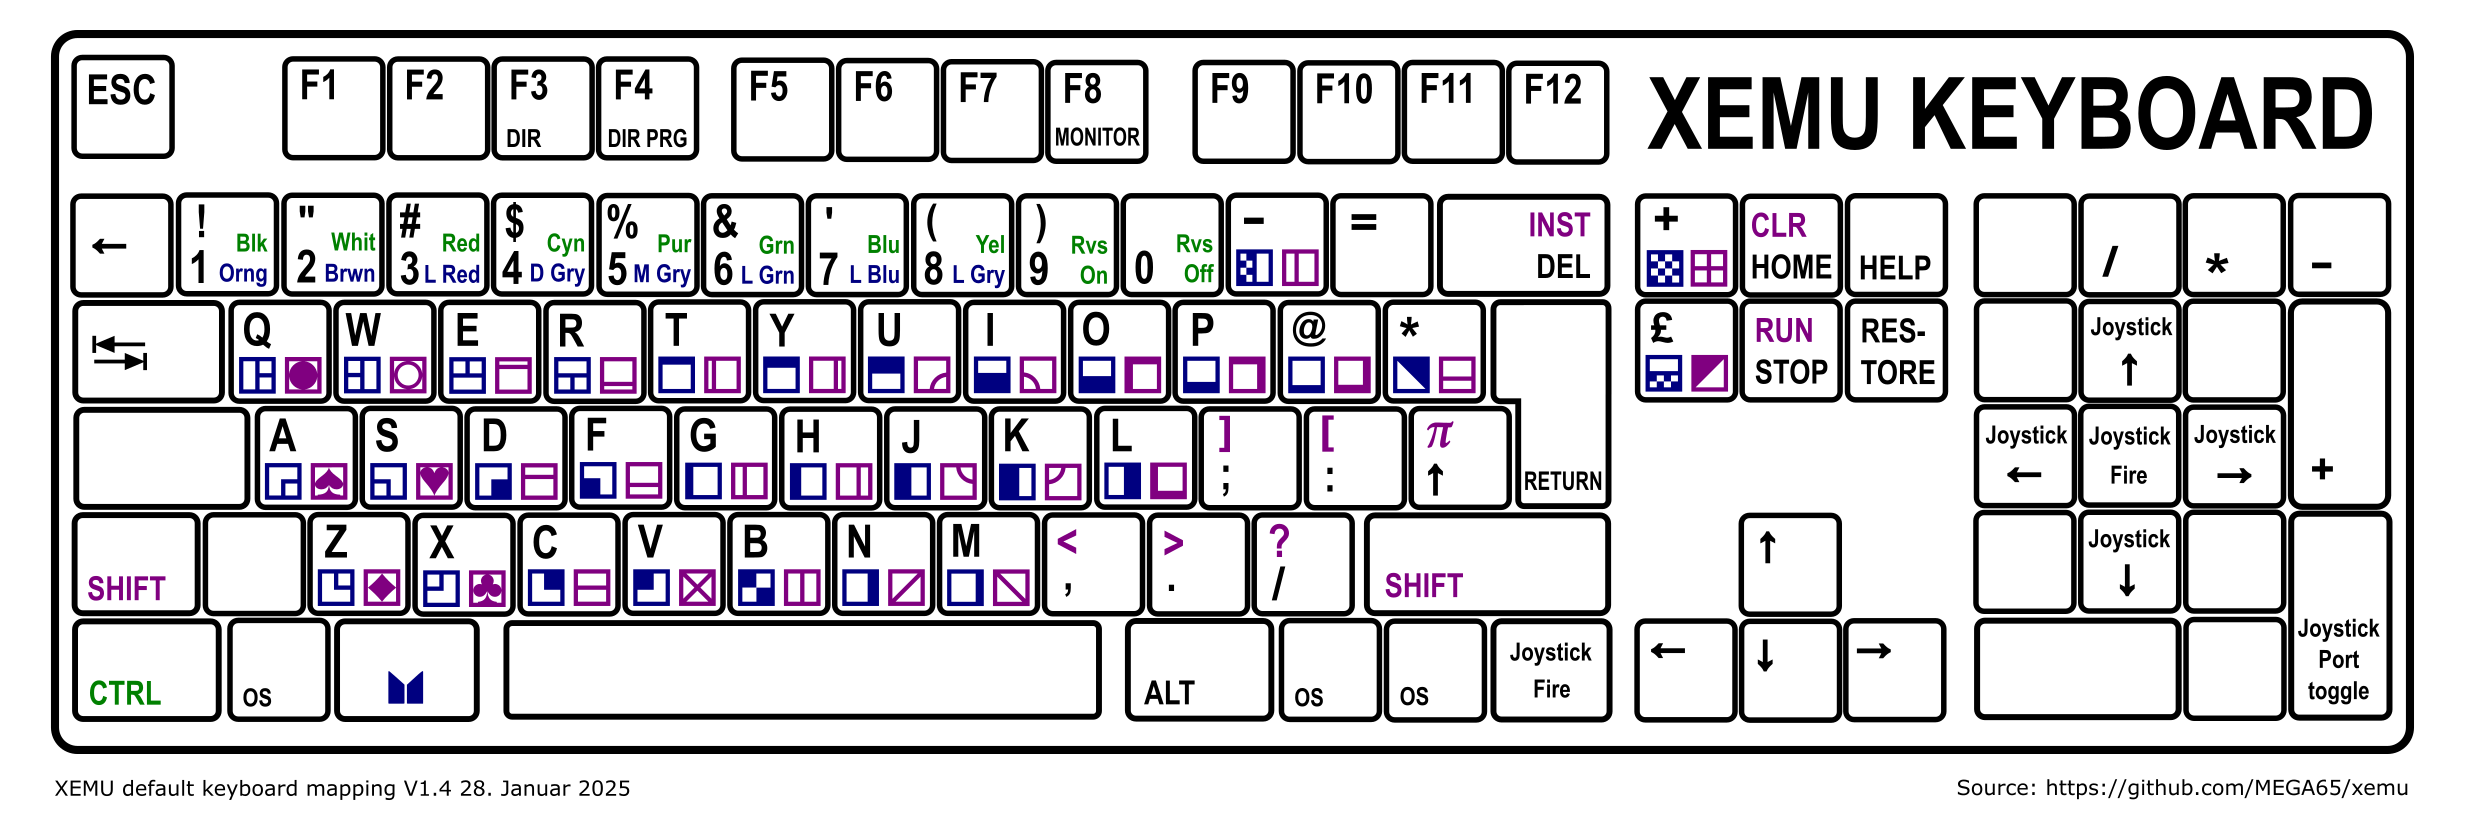
\includegraphics[width=\linewidth]{images/xemu-extended-keyboard.png}
\end{center}

On most PC keyboards, this places \specialkey{RUN STOP} and \widekey{RESTORE} next to each
other, to make that key combination easy to enter.

This diagram shows the PETSCII glyphs as they appear on a MEGA65 keyboard, with the
\megasymbolkey glyph on the left and the \specialkey{Shift} glyph on the right. Note
that on a PC keyboard, the key for \megasymbolkey is to the right of the
\specialkey{Shift}.

Xemu lets you have two joysticks (one at a time) on the numeric keypad.
\specialkey{Enter} over there is used to toggle ports 1, 2 and to off when pressed
repeatedly.

Please be aware the emulator by default catches \megakey{F9} \megakey{F10}
\megakey{F11} as shortcuts of its own functions. If you want to use these keys with the
emulated MEGA65, you must configure the keyboard mapping. The files are found in the
folder for Xemu's settings as explained on page
\pageref{sec:sdcard-settings-location}. This is done by copying
\stw{keymap-default.cfg} into \stw{keymap.cfg} and then removing the following lines:

\begin{tcolorbox}[colback=black,coltext=white]
\verbatimfont{\codefont}
\begin{verbatim}
XEMU-EXIT F9
XEMU-FULLSCREEN F11
\end{verbatim}
\end{tcolorbox}

and changing:

\begin{tcolorbox}[colback=black,coltext=white]
\verbatimfont{\codefont}
\begin{verbatim}
F9 Unknown
F11 Unknown
\end{verbatim}
\end{tcolorbox}

into:

\begin{tcolorbox}[colback=black,coltext=white]
\verbatimfont{\codefont}
\begin{verbatim}
F9 F9
F11 F11
\end{verbatim}
\end{tcolorbox}

With these keys remapped, the full-screen and exit functions are still available from
the menu. Right-click (or control-click) anywhere in the window to access it.

\subsection{Apple MacOS start problems}

If a message \stw{macOS cannot verify that this app is free from malware} pops up
use the following procedure when you open the app for the first time:\index{Apple}
\index{macOS}

\begin{itemize}
  \item Open Finder on your Mac.
  \item Control-click (or right-click) on the Xmega65 app icon.
  \item In the context menu, select \stw{Open}.
  \item The message appears again, but this time there is an \stw{Open} button.
        Click \stw{Open}. You only need to perform this procedure the first time you
		run the app. From now on, you can open the app normally.
\end{itemize}

\subsection{Updating settings}
\label{sec:sdcard-settings-location}
\index{SD card}

You may wish to edit the Xemu settings file to change the keyboard mapping or make
a backup of the SD card image file. To access these files from within Xemu, open the
menu, select \stw{Debug / Advanced} then \stw{Browse system folder}. Edit the
\stw{keymap-default.cfg} and \stw{mega65-default.cfg} files with a text editor.
For specific instructions on how to change \stw{keymap-default.cfg} please refer to
page \pageref{sec:xemu-keyboard}.

\begin{center}
  \includegraphics[width=0.5\linewidth]{images/xemusettings.png}
\end{center}

The Xemu system folder location varies by operating system:

\begin{itemize}
    \item Windows (may be copied into the address bar of the file explorer):
    \stw{\%appdata\%$\textbackslash$xemu-lgb$\textbackslash$mega65}
    \item Linux:
    \stw{$\textasciitilde$/.xemu-lgb/}
    \item Macintosh:
    \stw{$\textasciitilde$/Library/Application$\textbackslash$ Support/xemu-lgb/mega65/}
\end{itemize}

\section{Using the Live ISO image}
\label{sec:live-iso-image}

The Live ISO image is the product of a volunteer community; not the MEGA65 team. We include it for your convenience.

\subsection{Creating a Bootable USB stick or DVD}

There are many ways to create a live ISO image. The method you choose depends on your operating system and whether you wish to install to a USB drive or burn it to a DVD. Burning to a DVD is straightforward, assuming you own a computer that has a DVD writer. If you wish to create a faster bootable USB drive, try one of the methods below:

If you are using Windows, consider a tool like \url{http://www.isotousb.com/}.

On Linux, you can use the instructions at \url{https://fossbytes.com/create-bootable-usb-media-from-iso-ubuntu/}.

For Apple Macs, consider these instructions at
\url{https://ubuntu.com/tutorials/create-a-usb-stick-on-macos#1-overview}.

Similar instructions are available for other popular computers, such as Amigas (\url{https://forum.hyperion-entertainment.com/viewtopic.php?t=3857}), or Sun UltraSPARC workstations (\url{https://forums.servethehome.com/index.php?threads/how-to-create-a-bootable-solaris-11-usb.1998/}).

Finally, the popular, easy-to-use, and free cross-platform belanaEtcher is available at \url{https://www.balena.io/etcher/}.

\subsection{Getting Started}

To avoid potential copyright issues, the bootable ISO image does not include proprietary ROMs for the MEGA65; such as legacy C65 ROMs. It does include an open-source replacement ROM from our OpenROMs project.\index{OpenROMs} This ROM will boot into a BASIC 2 environment that you can use to load and execute many C64 programs as shown in the image below:

\screenshotwrap{images/liveiso-openrom.png}

If you wish to use a C65 ROM that includes BASIC 10, download the appropriate ROM file and place it on another USB stick named \stw{MEGA65.ROM}. On start-up, the MEGA65 will ask if a ROM has been downloaded; as shown in the image below:

\screenshotwrap{images/liveiso-rom-usb-prompt.png}

If the Live ISO cannot find a ROM, it will prompt you to download a ROM; as shown below:

\screenshotwrap{images/liveiso-rom-download-prompt.png}

\subsection{Other Features of the Live ISO}

As the previous screen-shots show, the Live ISO provides various and convenient desktop shortcuts. On the left-hand side, there are shortcuts for launching the
MEGA65 emulator and the C65 emulator so you can test that programs
will run on both platforms. As previously mentioned, both emulators are a work in progress and may not be 100\% compatible.

Another link provides access to the MEGA65 Book. This all-in-one volume, of apporixmately 800 pages, contains the official MEGA65 documentation. The majority of this developer's guide is also present in the MEGA65 Book.

This ISO also includes documentation for the C65 Notepad; a program for the C65 and MEGA65 written by Snoopy (the developer of the Live ISO image). A ``read me'' file contains further information about the Live ISO.

Finally, on the right-hand side, there are links to download a C65 ROM and to update the MEGA65 Book to the latest version. This will ensure you don't need to create a new bootable image each time a frequent update is made to the MEGA65 Book.

To access all contents of the Live ISO image, use the file explorer.

% 2022-11-28 edits by nobruinfo
% 2021-03-17 edits by SBC

\chapter{Data Transfer and Debugging Tools}
\label{cha:transfer-and-debug-tools}

The key to effective cross-platform development is having quick and
easy means to deploy and test software on the MEGA65.  This is
especially true while the MEGA65 emulator continues to be developed.
In fact, even once the MEGA65 emulator is complete, it is unlikely
that it will be able to offer full compatibility at full speed,
because the MEGA65 is much more demanding to emulate than the C64.

There are a variety of tools that can be used for data transfer and
debugging.  These typically function using either the MEGA65's serial
monitor interface, or via the MEGA65's fast ethernet adapter.  The
serial monitor interface is available via the UART lines on the JB1
header.

If you do not have access to the serial monitor interface, there are
tools being developed for the fast ethernet port that provide some,
but not all, of the capabilities of the serial monitor
interface. These will be documented as they become available. The
remainder of this chapter focusses on methods that access the serial
monitor interface.

You can either connect a 3.3V UART adapter to the appropriate
lines, or more conveniently, connect a TE-0790-03 JTAG debug module
onto this connector.  This gives you a USB connection that can be used
for injecting software, remote debugging and memory inspection, as
well as activating or flashing bitstreams.  With this connection,
there are the following tools:

\section{m65 command line tool}

The \url{https://github.com/mega65/mega65-tools} repository contains a
number of tools, utilities and example programs. These tools are mainly for Linux but can be used on Windows with Cygwin. One of those is
the \stw{m65} command line tool. This is rather a swiss-army
knife collection of utilities in one.  Common useful functions
include:

\subsection{Screenshots using m65 tool}

To take a screenshot of the MEGA65 use:

\begin{screenoutput}
m65 -S
\end{screenoutput}

This will create a file called \stw{mega65-screeen-000000.png},
or if that file already exists, the first non-used number will be used
in place of \stw{000000}.

Note that this screenshot function works by having \stw{m65} emulate the
function of the VIC-IV. Thus while it produces excellent looking
digital screenshots, it may not exactly match the real display of the
MEGA65.  At the time of writing it does not render sprites or
bitplanes, only text and bitmap-based video modes.

\subsection{Load and run a program on the MEGA65}

To load and run a program on the MEGA65, you can use a command like:

\begin{screenoutput}
m65 -F -4 -r foo.prg
\end{screenoutput}

The \stw{-F} option tells \stw{m65} to reset the MEGA65
before loading the program.

The \stw{-4} option tells \stw{m65} to switch the MEGA65
to C64-mode before loading the program. If this is left off, then it
will attempt to load the program in C65-mode.

The \stw{-r} option tells \stw{m65} to run the program
immediately after loading.

Note that this command works using the normal BASIC LOAD command, and
is thus limited to loading programs into the lower 64KB of RAM

\subsection{Reconfigure the FPGA to run a different bitstream}

To try out a different MEGA65 bitstream, a command like the following can be
used:

\begin{screenoutput}
m65 -b bitstream.bit
\end{screenoutput}

This will cause the named bitstream to be sent to the FPGA.  As the
FPGA will be reconfigured by this action, and program currently
running will not merely be stopped, but also main memory will be
cleared. For models of the MEGA65 that are fitted with 8MB or 16MB of
expansion memory, those expansion memories are implemented in external
chips, and so the contents of them will not be erased.

For non-MEGA65 bitstreams (such as zxunomega65 and gbc4mega65), use the '-q' argument instead:

\begin{screenoutput}
m65 -q bitstream.bit
\end{screenoutput}

\subsection{Remote keyboard entry}

The MEGA65's keyboard interface logic supports the injection of
synthetic key events using the registers \$D615 -- \$D617.
The \stw{m65} utility uses this to allow remote typing on the MEGA65
in a way that is transparent to software.  There are three ways to use
this:

\begin{screenoutput}
m65 -t sometext
\end{screenoutput}

This form types the supplied text, in this case {\em sometext}, but
does not simulate pressing \specialkey{RETURN}.  If you wish
to simulate the pressing of \specialkey{RETURN}, use \stw{-T}
instead of \stw{-t}, e.g.:

\begin{screenoutput}
m65 -T list
\end{screenoutput}

This would cause the LIST command to be typed and executed.

Finally, it is possible to begin general remote keyboard control via:

\begin{screenoutput}
m65 -t -
\end{screenoutput}

In this mode, any key pressed on the keyboard of the computer
where \stw{m65} is running will be relayed to the MEGA65.  Note that
not all special keys are supported, and that there is some latency, so
using key repeat can cause unexpected results.  But for general remote
control, it is a very helpful facility.

\subsection{Unit testing and logging support}

The \stw{m65} tool includes support to facilitate remote unit testing 
directly on MEGA65 hardware. When \textit{unit testing mode} is active, 
\stw{m65} waits for the MEGA65 to send certain byte sequences over the 
serial interface which signal the current state (started, passed, failed) 
of a given test. Additionally, it is possible to send log messages from 
the MEGA65 to the host computer.

Unit testing mode is entered by calling \stw{m65} with the \stw{-u} flag. 
To run a remote BASIC program in C65-mode and simultaneously put \stw{m65}
into \textit{unit testing mode}, the following command can be used:

\begin{screenoutput}
    m65 -Fur attic-ram.prg -w tests.log
\end{screenoutput}

The \stw{-F} and \stw{-r} options tell \stw{m65} to reset the MEGA65
before loading the program "attic-ram.prg" and then automatically run it. 
The \stw{-u} option then tells \stw{m65} go into \textit{unit testing mode} 
instead of exiting after launching the program.
The optional \stw{-w} option makes \stw{m65} append the test results to the 
file "test.log" (creating the file if it doesn't exist). 

Please note that \stw{m65} automatically exits from \textit{unit testing mode}
if no test state signals were received for over 10 seconds.

Support is provided for sending unit test signals to the host computer from
C and BASIC 65 programs:

\subsubsection{Using unit tests with C}

The MEGA65 libc contains support for unit testing via functions defined in 
\stw{tests.h} and \stw{tests.c}. 

To signal the start of a test, include \stw{tests.h} and use

\begin{verbatim}
    unit_test_setup("testName",issueNumber);
\end{verbatim}

where \textit{"testName"} is a human-readable name of the test (e.g. 
"VIC-II") and \textit{issueNumber} a reference to the corresponding
bug issue (for example, the issue number from github).

After starting a test, it's possible to signal passed tests with 
the unit\_test\_ok() function:

\begin{verbatim}
    unit_test_ok();
\end{verbatim}

A failed test is signalled with unit\_test\_fail():

\begin{verbatim}
    unit_test_fail("fail message");
\end{verbatim}

Each time the unit\_test\_ok() or unit\_test\_fail() 
functions are called, the \textit{sub issue} of the test (reported on 
the host computer) is incremented. This makes it easier to combine and 
identify multiple tests in one file.

You can send arbitrary log messages via unit\_test\_log():

\begin{verbatim}
    unit_test_log("hello world from mega65!");
\end{verbatim}

...and finally, when all is done, the end of unit testing is signalled
by the use of

\begin{verbatim}
    unit_test_done();
\end{verbatim}


\subsubsection{Using unit tests with BASIC 65}

\stw{b65support.bin} is a machine language module providing support for 
unit testing from BASIC 65, available in the \stw{bin65} folder of the mega65-tools
repository. This module works by redirecting the USR vector to perform the functions 
needed to communicate with the testing host.

In an automated test scenario, you may want to inject the \stw{b65support.bin} 
binary into MEGA65 RAM by using \stw{m65}:

    \begin{screenoutput}
        m65 -@ mega65-tools/bin65/b65support.bin@15fe
    \end{screenoutput}


Of course it's also possible to load \stw{b65support.bin} directly from the
MEGA65 by mounting the \stw{M65UTILS.D81} image from the freezer and issuing

\begin{screenoutput}
    BLOAD "B65SUPPORT.BIN"
\end{screenoutput}

After loading, \stw{b65support.bin} is initialized with

\begin{screenoutput}
    SYS $1600
\end{screenoutput}

Once initialized, the following functions are provided by \stw{b65support.bin}:

\begin{screenoutput}
    A=USR(<issueNum>)
\end{screenoutput}
prepares a new test with number <issueNum> and resets subissue number to 0

\begin{screenoutput}
    A=USR("=<testName>")
\end{screenoutput}
sets test name and sends test start signal; for example: \stw{A=USR("=VIC-III")} 
sets the test name to 'VIC-III' and signals the host computer that the test 
has started.

\begin{screenoutput}
    A=USR("/<logMessage>)
\end{screenoutput}
sends a log message to the host computer

\begin{screenoutput}
    A=USR("P")
\end{screenoutput}
sends the 'passed' signal to the host computer and increases the sub issue number

\begin{screenoutput}
    A=USR("F")
\end{screenoutput}
sends the 'test failed' signal to the host computer and increases 
the sub issue number

\begin{screenoutput}
    A=USR("D")
\end{screenoutput}
sends the 'test done' signal to the host computer 

All calls return the current sub issue number or \stw{?ILLEGAL QUANTITY ERROR} in 
case of calling an invalid command.

\subsubsection{BASIC 65 example}

The following is a complete BASIC 65 example showing how to use \stw{m65}'s
unit testing features:

\begin{screenoutput}
    100 rem attic ram cache test
    110 poke $bfffff2,$e0         : rem enable attic ram cache
    120 sys $1600                 : rem init test module
    130 a=usr(379)                : rem set issue number
    140 a=usr("=attic-ram-cache") : rem set test name
    150 bank128:poke0,65          : rem just to be sure
    160 b0=$8000000 : b1=$8000100 : rem attic ram areas to be tested
    170 for r=0 to $ff
    180   poke b0+r,0             : rem fill area 1 with 0
    190   poke b1+r,$ff           : rem fill area 2 with $ff
    200 next r
    210 for t=1 to 10             : rem 10 tries
    220   poke b0,32              : rem write to b0
    230   for x=0 to $ff:t1=b1+x
    240     a=peek(b0)            : rem read from b0
    250     b=peek(t1):b=peek(t1) : rem read twice from t1
    260     ifb<>255 thenf=t:t=11:x=256   : rem this shouldn't happen
    270   next x
    280 next t
    290 if f=0 then begin
    300   print "no faults detected after";t;"tries."
    310   a=usr("p")              : rem signal 'test passed' to host
    320 bend : else begin
    330   a=usr("f")              : rem signal 'test failed' to host
    340   print "hyper ram fault detected after";f;"tries."
    350   print "peek($";hex$(t1);") [t1] is";b;"but should be 255"
    360 bend
    370 a=usr("d")                : rem test done    
\end{screenoutput}

\section{M65Connect}

This is a cross-platform graphical tool available for Windows, Linux
and MacOSX, which allows access to most of the functions of
the \stw{m65} command-line tool, without needing to use a
command line, or being able to compile the tool for your preferred
operating system.

The repository for M65Connect is: \url{https://github.com/MEGA65/m65connect}

The latest binary version is available from \url{https://files.mega65.org}.

With the MEGA65 or Nexys FPGA switched off, connect a USB cable from your computer to the MEGA65 or Nexys FPGA board. Run the \textit{M65Connect} executable and follow the prompts to connect. The program will help you identify which USB Serial Port to communicate over.

With this tool you can easily transfer PRG programs and a variety of other files. M65Connect can handle the transfer, switching to C64-mode, and execution of programs.

\section{mega65\_ftp}

The \stw{mega65}\_\stw{ftp} utility from
the \url{https://github.com/mega65/mega65-tools} repository is a
little misleadingly named: While it 
is a File Transfer Program, it does not use the File Transfer
Protocol (FTP).  Rather, it uses the serial monitor interface to take
remote control of a MEGA65, and directly access its SD card to enable
copying of files between the MEGA65 and the host computer.

Note that it does not perfectly restore the MEGA65's state on exit,
and thus should only be used when the MEGA65 is at the READY prompt,
so that any running software doesn't go haywire. In particular, you
should avoid using it when a sensitive program is running, such as
the Freeze Menu, MEGA65 Configuration Utility, or the MEGA65
Format/FDISK utility.  (This problem could be solved with a little
effort, if someone has the time and interest to fix it).

When run, it provides an FTP-like interface that supports
the \stw{get}, \stw{put}, \stw{rename} and \stw{dir} commands.
Note that when putting a file, you should make sure that it is given a
name that is all capitals and has o DOS-compatible 8.3 character file
name.  This is due to limitations in both \stw{mega65}\_\stw{ftp} and the
MEGA65's Hypervisor's VFAT32 file system code. Again, these problems
could be fixed with a modest amount of effort on the part of a
motivated member of the community.

Finally, the \stw{mega65}\_\stw{ftp} program is {\em very} slow to push
new files to the MEGA65, typically yielding speeds of around 5KB/sec.
This is partly because the serial monitor interface is capable of
transferring data at only 40KB/sec (when set to 4,000,000 bits per
second), and partly because the remote control process results in a
lot of round-trips where helper routines are executed on the MEGA65 to
read, write and verify sectors on the SD card.  It would be quite
feasible to improve this to reach close to 40KB/sec, and potentially
faster using either some combination of data compression,
de-duplication of identical sectors (especially when uploading disk
images) and other techniques. Again, this would be a very welcome
contribution that someone in the community could contribute to
everyone's benefit.

\section{TFTP Server}

Work on a true TFTP server for the MEGA65 that supports fast
TFTP transfers over the 100mbit ethernet has begun, and can be used to
very quickly read files from the MEGA65. Speeds of close to 1MB/sec
are possible, depending on SD card performance.  Rather than using
DHCP, this utility will respond to {\em any} IP address that ends in
.65. It always uses the MAC address 40:40:40:40:40:40. True DHCP
support as well as using the MEGA65's configured ethernet MAC address
may be added in the future. 

More importantly, support for writing
files to the SD card is not yet complete, and is blocked by the need
for the implementation of the necessary functions in the MEGA65's Hypervisor for creating and
growing files.  A particular challenge is enabling the creation of
files with contiguous clusters as is required for D81 disk images: If
a D81 file is fragmented, then it cannot be mounted, because the
mounting mechanism requires a pointer to the contiguous block of the
SD card containing the disk image.
In the interim, \stw{mega65}\_\stw{ftp} can be used as a substitute.

\section{Converting a BASIC text file listing into a PRG file}

If you have a untokenised BASIC program in plain text format sourced from somewhere like an internet post, and you wish to try it on the MEGA65 without typing it in, it is possible to convert it to a PRG.

\textit{C64List} is a Windows-based command-line tool that will allow you to make the conversion. Once you have a \textit{.PRG} file, you can use a tool like M65Connect to upload it to the MEGA65 or Nexys FPGA. 

C64List is available for download from \url{http://www.commodoreserver.com/Downloads.asp}

Ensure you have a program listing saved to a file on your local computer (for example, \textit{program.txt}) encoded as ANSI or UTF8.

Use C64List to convert the file to a PRG file using:
    
\begin{tcolorbox}[colback=black,coltext=white]
    \begin{verbatim}
        C64List program.txt -prg
    \end{verbatim}
\end{tcolorbox}

Now you can upload your newly converted program to the MEGA65 with M65Connect or one of the other tools described previously.

It is worth noting that this method will not be 100\% effective on listings with special PETSCII characters. Programs with PETSCII will require some editing on the MEGA65 itself before saving to disk.

\chapter{Assemblers}

The table below shows an overview of assemblers known to work with MEGA65.
For general use we recommend {\bf ACME} as it has good support
for the 45GS02 instruction set; is open source; and finally written in C. The latter
means that it may be ported to run natively on the MEGA65 in the future.

\begin{longtable}{ | l | l | l | l |}\hline
Name     & 45GS02 & Source & Reference \\\hline
ACME     &  yes   & C      & \url{https://sourceforge.net/projects/acme-crossass}\\
KickAss  &  yes   & Java   & \href{https://gitlab.com/jespergravgaard/kickassembler65ce02}{gitlab.com/jespergravgaard/kickassembler65ce02}\\
Ophis    &  yes   & Python & \url{https://github.com/michaelcmartin/Ophis}\\
BSA      &  yes   & C      & \url{https://github.com/Edilbert/BSA}\\
CA65     &  no\footnote{Our fork of CA65 (part of CC65) correctly detects the MEGA65's CPU, but has no explicit support for the processor's features} & C & \url{https://github.com/mega65/cc65}\\\hline
\end{longtable}

The {\bf BSA} assembler is currently used to build the {\bf MEGA65.ROM}.
Most of this source code is written in the syntax
of the ancient {\bf BSO} assembler (Boston Systems Office), which was used in the
years 1989 - 1991 by software developers, working on the C65.
The {\bf BSA} Assembler has a compatibility mode, which makes it
possible to assemble these old source codes with minor or none modifications.
The {\bf BSA} Assembler has currently only a description of commands
embedded in the C-source of the assembler.

%Therefore a chapter, describing the usage and the features of {\bf BSA}
%is started after this chapter and will be completed during the next weeks.


\chapter{C and C-Like Compilers}

Short answer: CC65 and KickC both work on the MEGA65.

Both CC65 and KickC are known to work on the MEGA65.  However, both by
default have only a C64 memory model, and use only 6502 opcodes.
It would be super for someone to create a C65 memory configuration for
CC65, and should not be too hard to do.

CC65 supports overlays, which
could be powerfully used with the MEGA65's extra memory to allow
programmes larger than 64KB.  However, this would require writing a
suitable loader for such programmes, which also does not yet exist.

Similarly, modifying the code
generator of CC65 to use 45GS02 features would not be particularly
difficult to do, and would help to overcome the otherwise horribly
slow and bloated code that CC65 produces.  Also adding first-class
support for the 45GS02 CPU features in CA65 (or perhaps even better,
making CC65 produce ACME compatible assembly output) would be of
tremendous advantage, and not particularly hard to do.  These would
all be great tasks to tackle while you wait for your MEGA65 DevKit to
arrive!

An example template for a C program that can be compiled using CC65
and executed on the MEGA65 can be found in the repository
\url{https://github.com/MEGA65/hello-world}.  This repository will
even download and compile CC65, if you don't already have it installed
on your system.  This repository should work on Linux and Mac, and
on Windows under the Windows Subsystem for Linux (WSL).

\section{MEGA65 libc}

A C library is being developed for the MEGA65, and which already
includes a number of useful features. This library is available from
\url{http://github.com/mega65/mega65-libc}. The procedures,
functions and definitions it provides are documented in a separate
chapter.

The MEGA65 libc is currently available only for CC65, although we would
welcome someone maintaining a KickC port of it.

\chapter{MEGA65 Standard C Library}

A C library is being developed for the MEGA65, and which already
includes a number of useful features. This library is available from
\url{http://github.com/mega65/mega65-libc}. The procedures,
functions and definitions it provides are documented in a separate
chapter.

The MEGA65 libc is currently available only for CC65, although we would
welcome someone maintaining a KickC port of it.

\section{Structure and Usage}

The MEGA65 libc is purposely provided in source-form only, and with groups
of functions in separate files, and with separate header files for including.
The idea is that you include only the header files that you require, and
add only the source files required to the list of source files of the program
you are compiling.  This avoids the risk of the compiler including functions
in your compiled program that are never used, and thus wasting precious memory
space.

Note that some library source files are written in C, and thus are present as
files with a \stw{.c} extension, while others are written in assembly language
either for efficiency or out of necessity, and have a \stw{.s} extension.

Typical usage is to either have the mega65-libc source code checked out in an
adjacent directory, or within the source directory of your own project.  In the
latter case, this can be done using the git submodule facility.

The following sections document each of the header files and the corresponding
functions that they provide.

\section{conio.h}

\titleformat*{\subsection}{\normalfont\huge\bfseries\color{blue}}

\input{api-conio}

\subsection{VIC\_BASE}

{\em VIC\_BASE} is a pre-processor macro that provides the base address of the
VIC-IV chip, i.e., \$D000.

{\em IS\_H640} is a pre-processor macro that returns 0 if the current VIC-III/IV
video mode is set to 320 pixels accross (40 column mode), and non-zero if it is set to 640 pixels across (80 column mode).

\chapter{BASIC Tokenisers}

Various tokenisers for C64 BASIC exist, e.g., \url{https://github.com/catseye/hatoucan},
\url{https://www.c64-wiki.com/wiki/C64list}, or the \stw{petcat} utility that is part of VICE.
If you are using Ubuntu Linux, you can install \stw{petcat} by using the following command:

\begin{screenoutput}
sudo apt-get install vice
\end{screenoutput}

We recommend \stw{petcat}, because it supports both C64 BASIC 2 and C65 BASIC 10.

Some IDEs offer BASIC 65 tokenisers within them, such as:

\stw{Eleven}

\url{https://files.mega65.org?id=8b189d0b-ea1e-45a7-a4de-87bcb0b11696}

\stw{C64 Studio}

\url{https://www.georg-rottensteiner.de/files/C64StudioRelease.zip}

\stw{CBM prg Studio}

\url{https://www.ajordison.co.uk}


\part{NATIVE DEVELOPMENT TOOLS}

\chapter{C65 Memory Monitor}

\chapter{MEGA65 Matrix Mode}

\chapter{Turbo Assembler}

\chapter{Dealing with C65 and C64-mode}

The MEGA65 normally starts in C65-mode, and there is appeal in making
programs that can start directly from C65-mode.  However, the
different versions of the C65 ROM make this difficult, as there are
differences in the memory location of various system variables and ROM
routines.  If you are developing a program in assembly language or
C, it is typically easier to develop it for C64-mode.

But that leaves
you with the problem of how to allow it to be started from C65-mode.
Our solution to this is the \stw{c65toc65wrapper.asm} program.  This
short program can be found in the \stw{src/utilities} directory of
the \url{https://github.com/mega65/mega65-tools} repository.  When
compiled, it produces a short program that you can pre-pend to your
C64-mode oriented MEGA65 program, and have it automatically detect
C64 or C65-mode, switch to C64-mode if required, and set your
program going. It also switches the CPU to 40MHz.  The only
assumption it makes, is that your program should be started using
\stw{SYS 2061}

This program is particularly handy when using exomizer, as by having
the CPU set to 40MHz before depacking allows depacking to happen
almost instantly.  This is important on the MEGA65, as loading a
program often takes only a fraction of a second, but depacking an
exomized program at 1MHz can take several seconds.

Finally, you can use this approach to create bootable disks for the
MEGA65, by placing the file onto the disk with the
name \stw{AUTOBOOT.C65}.  This allows you to use C64-mode programs
to autoboot on the MEGA65, which is itself very convenient.

\part{MEGA65 Operating System}

\chapter{Developing System Programmes}

\section{Introduction}

The MEGA65 has a number of system programs and utilities that are used at various times to perform various functions.
This includes the utilities accessible via the Utility Menu \index{Utility Menu}, the Freeze Menu \index{Freeze Menu} and
its own helper programs, as well as the Flash Menu \index{Flash Menu}\index{MEGA Flash}.

A number of these system programs are pre-loaded into the MEGA65 bitstream, while others live on the SD card.
For those that are pre-loaded into the MEGA65 bitstream, this works by having areas of pre-initialised memory, that
contain the appropriate program.  For example, the utilities accessible via the Utility Menu are all located in
the colour RAM, while the Flash Menu is located at \$50000 -- \$57FFF.

In one sense, the easiest way to test new versions of these utilities is to generate a new bitstream with the updated versions.
However, synthesising a new bitstream is very time consuming, typically taking an hour on a reasonably fast computer.
Therefore this chapter explains the procedure for loading an alternate version of each of these system programs, as well as
providing some useful information about these programs, how the operate, and the environment in which they operate compared
with normal C64 or C65-mode programs.

\section{Flash Menu}

The flash menu is located in pre-initialised RAM at \$50000 -- \$57FFFF.  It is executed during the first boot each time the
MEGA65 is switched on.  It is unusual in that it executes in the hypervisor context. This is so that it has access to
the QSPI
flash, which is not available outside of Hypervisor Mode, so that user programs cannot corrupt the cores stored in the flash.

It is also important to note that the flash menu program must fit {\em entirely} below \$8000 when loaded {\em and} executing, as the Hypervisor is still mapped at \$8000 -- \$BFFF, and can easily be corrupted by an ill behaved flash menu program.  In this regard, the flash menu
can be regarded as an extension of the hypervisor that is discarded after the first boot.
This is unlike all other system programs, that operate in a dedicated memory context, from where the Hypervisor is safe from corruption. It also means that you can't crunch the flash menu to make it fit, as it would overwrite the Hypervisor during decrunching.

Also, as the flash menu is executed very early in the boot process, only the pre-included OpenROM ROM image is available.  Thus you must ensure that your flash menu program is compatible with that ROM.

The Hypervisor maintains a flag that indicates whether the flash menu has been executed or not. This flag is updated at the point
where the Hypervisor exits to user mode for the first time, since after that point, the contents of \$50000 -- \$57FFF can no longer
be trusted to contain the flash menu.  This means that if you wish to have the Hypervisor run a new version of the flash menu that
you have loaded, you must prevent the Hypervisor from exiting to user mode first.

The easiest way to achieve this is to hold the ALT key down while powering on the MEGA65.  This will cause the Hypervisor to display the Utility Menu, rather than exiting to user mode.  It is safe at this time to use the {\tt m65} utility to load the replacement flash menu program using a command similar to the following:

\begin{tcolorbox}[colback=black,coltext=white]
\verbatimfont{\codefont}
\begin{verbatim}
m65 -@ newflashmenu.prg@50000
\end{verbatim}
\end{tcolorbox}

That command would load the file {\tt newflashmenu.prg} at memory location \$50000.

After that, you can simply press the reset button on the side of the MEGA65 while holding \specialkey{NO SCROLL} down,
and it will boot again, and because it never left Hypervisor Mode during the previous boot cycle, it will run your
updated flash menu program.

It should also be possible to completely automate this process, by first using {\tt m65 -b} to load a new bitstream, thus simulating a cold boot, and then quickly calling {\tt m65} again to simulate depressing the ALT key (or herhaps simply halting the processor), then {\tt m65 -@ ...} and finally {\tt m65 -F} to reset the machine.  Writing a script or utility that correctly implements this automation is left as an exercise for the reader.

\section{Format/FDISK Utility}

The Format/FDISK utility is accessed as part of the Utility Menu system.  These utilities are compiled, crunched and linked using the
{\tt utilpacker} program.  If you have checked out the mega65-core source repository, you can re-build the colour RAM image by using:

\begin{tcolorbox}[colback=black,coltext=white]
\verbatimfont{\codefont}
\begin{verbatim}
make bin/COLOURRAM.BIN
\end{verbatim}
\end{tcolorbox}

You will of course need to first have modified the Format/FDISK utility, which is normally located in the {\tt src/mega65-freeze-menu} subdirectory.

You need to then load this modified colour RAM image into the running machine. Similar to when updating the flash menu, the Hypervisor will
only present the utility menu on the first boot, before exiting to user mode for the first time, because it cannot otherwise be sure that
the colour RAM contains the valid utility programs.  

So as for the flash menu, you would power the MEGA65 off, and then holding the ALT key down, you switch the MEGA65 back on, so that it displays the utility menu.  At this point you can use the following command to load your modified {\tt COLOURRAM.BIN} file:

\begin{tcolorbox}[colback=black,coltext=white]
\verbatimfont{\codefont}
\begin{verbatim}
m65 -c COLOURRAM.BIN
\end{verbatim}
\end{tcolorbox}

You can now hold \specialkey{ALT} down, and press the reset button on the left-hand side of the MEGA65, which should
again present
the utility menu,
but this time with your modified format/fdisk utility in place.

\section{Keyboard Test Utility}

The process for updating the Keyboard test utility is essentially the same as for the format/FDISK utility, as it lives in the colour RAM

\section{MEGA65 Configuration Utility}

The process for updating the MEGA65 Configuration utility is essentially the same as for the format/FDISK utility, as it lives in the colour RAM

\section{Freeze Menu}

The Freeze Menu is a normal program, which is stored in {\tt FREEZER.M65} on the SD card's FAT32 file system.

To updated the Freeze Menu, simply use the {\tt m65ftp} utility or some other means to upload your updated FREEZER.M65 file to the SD card's FAT32 file system.  The format of the program is simply a C64-mode PRG file, just renamed to FREEZER.M65.

\section{Freeze Menu Helper Programmes}

The Freeze Menu helper programs are updated in the same way as the Freeze Menu itself.

\section{Hypervisor}

The Hypervisor is normally built as HICKUP.M65, a 16KB file that contains the complete Hypervisor program.  MEGA65 bitstreams contain a pre-build version located at \$FFF8000 -- \$FFFBFFF.  Updated versions of the Hypervisor can be tested using two main approaches:

\begin{itemize}
	\item 1. Place the updated HICKUP.M65 file on the FAT32 file system of the SD card, and then power the MEGA65 off and on.  This works because the Hypervisor contains code that checks for an updated version of itself, and if found, loads it. However this approach is problematic in that if you install a newer bitstream, it will still downgrade the Hypervisor to whatever version is found in the HICKUP.M65 file on the SD card.  This method is only recommended for developers who have a need to test their modified Hypervisor code from a cold start. Even then, it is recommended to remove the HICKUP.M65 file immediately after testing to avoid unexpected down-grading in the future.
	\item 2. Use the m65 command's {\\t -k} option to replace the Hypervisor in place, and then reset the MEGA65 using the reset button on the left-hand side of the case.  This should be done when the Hypervisor is {\em not} active, so that corruption of current execution cannot occur. However, it must also occur before any ROM has been loaded to replace the default OpenROM image.  This is because the Hypervisor will attempt to call into the ROM on first-boot in prepration for calling the flash menu, and assumes that the OpenROM is present, because it uses a special OpenROM-specific call to initialise parts of the system state for the flash menu.  This is best done by using a command like {\tt m65 -k bin/HICKUP.M65 -R bin/MEGA65.ROM} to load both a new Hypervisor program and re-load an OpenROM image.
\end{itemize}

\section{OpenROM}

To load a new version of a ROM, there are several options, including replacing both the Hypervisor and ROM at the same time, as described above. However, typically the easiest is to copy the new ROM onto the FAT32 filesystem of the SD card as either MEGA65.ROM, or MEGA65$x$.ROM, where $x$ is replaced by a digit between 0 and 9.  When reseting the MEGA65, MEGA65.ROM will then be loaded as normal, or if a digit between 0 and 9 is held down on the keyboard while resetting, the Hypervisor will instead load MEGA65$x$.ROM, where $x$ is the number being held down on the keyboard.


{\newenvironment{hyppotrap}[3]
{
  \newcommand{\availablefrom}[1]{Available since Hyppo ##1}
  \newcommand{\deprecatedfrom}[1]{
    \textcolor{Orange}{
      \textbf{DEPRECATED} since Hyppo ##1.
      This service may be removed in a future version. New programs should
      not use this service.
    }
  }
  \newcommand{\errordesc}[3]{
    \index{Hyppo Error Codes!\$##1}
    \textbf{\$##1 ##2} ##3\par
  }
  \newcommand{\hypporef}[1]{
    \StrDel{hyppo:##1}{\_}[\reflbl]
    \nameref{\reflbl}
  }
  \newcommand{\notimplemented}{\item[Remarks:]\textbf{NOT IMPLEMENTED}\par}
  \newcommand{\register}[2]{\textbf{##1} ##2\par}
  \newcommand{\TODO}{\textbf{\color{red}TODO}}
  \titleformat*{\subsection}{\normalfont\huge\bfseries\color{blue}}
  \subsection{hyppo\_#1}
  { \StrDel{hyppo:#1}{\_}[\reflbl] \label{\reflbl} }
  \index{Hyppo Services!\$#2 \$#3}
  \begin{description}[leftmargin=2.7cm,style=nextline]
  \item [Trap:] LDA \#\$#3 : STA \$#2 : CLV
}
{
  \end{description}
}

\DeclareTCBInputListing{\acmelisting}{ m }{
  bottom=0mm,
  breakable,
  colback=black,
  coltext=lightgray,
  enhanced,
  frame empty,
  fontupper=\codefont,
  listing engine=listings,
  listing file={#1},
  listing only,
  listing options={
    basewidth=0.3em,
    breakatwhitespace,
    breakindent=0pt,
    breaklines,
    columns=fullflexible,
    commentstyle=\sffamily\footnotesize\color{Dandelion},
    includerangemarker=false,
    inputpath="examples/appendix-hypervisor-calls",
    keywordstyle={*\color{white}},
    keywordstyle={[2]\color{GreenYellow}},
    language={[acme]Assembler},
    linerange=EXAMPLE\ BEGINS-EXAMPLE\ ENDS,
    postbreak={;\space},
    rangeprefix=;\ >>>\ ,
    showstringspaces=false,
  },
  top=0mm,
  underlay first and middle={
    \node at ([yshift=-3mm]frame.south)
      {\ldots{} continues on the next page \ldots} ;
  }
}


\addtocontents{toc}{\protect\setcounter{tocdepth}{1}}
\chapter{MEGA65 Hyppo Services}
\index{Hyppo Services}
\index{Registers!\$D640}
\index{Registers!\$D641}
\index{Registers!\$D642}
\index{Registers!\$D643}
\index{Registers!\$D644}
\index{Registers!\$D645}
\index{Registers!\$D646}
\index{Registers!\$D647}
\index{Registers!\$D648}
\index{Registers!\$D649}
\index{Registers!\$D64A}
\index{Registers!\$D64B}
\index{Registers!\$D64C}
\index{Registers!\$D64D}
\index{Registers!\$D64E}
\index{Registers!\$D64F}
\index{Registers!\$D650}
\index{Registers!\$D651}
\index{Registers!\$D652}
\index{Registers!\$D653}
\index{Registers!\$D654}
\index{Registers!\$D655}
\index{Registers!\$D656}
\index{Registers!\$D657}
\index{Registers!\$D658}
\index{Registers!\$D659}
\index{Registers!\$D65A}
\index{Registers!\$D65B}
\index{Registers!\$D65C}
\index{Registers!\$D65D}
\index{Registers!\$D65E}
\index{Registers!\$D65F}
\index{Registers!\$D660}
\index{Registers!\$D661}
\index{Registers!\$D662}
\index{Registers!\$D663}
\index{Registers!\$D664}
\index{Registers!\$D665}
\index{Registers!\$D666}
\index{Registers!\$D667}
\index{Registers!\$D668}
\index{Registers!\$D669}
\index{Registers!\$D66A}
\index{Registers!\$D66B}
\index{Registers!\$D66C}
\index{Registers!\$D66D}
\index{Registers!\$D66E}
\index{Registers!\$D66F}
\index{Registers!\$D670}
\index{Registers!\$D671}
\index{Registers!\$D672}
\index{Registers!\$D673}
\index{Registers!\$D674}
\index{Registers!\$D675}
\index{Registers!\$D676}
\index{Registers!\$D677}
\index{Registers!\$D678}
\index{Registers!\$D679}
\index{Registers!\$D67A}
\index{Registers!\$D67B}
\index{Registers!\$D67C}
\index{Registers!\$D67D}
\index{Registers!\$D67E}
\index{Registers!\$D67F}

\section{Introduction}
A part of the MEGA65 is the system program called Hyppo that:
\begin{itemize}
  \item Boots the MEGA65.
  \item Loads the ROMs and other files from the SD card.
  \item Makes memory banks 2 and 3 ROM-like by protecting them from being
        written to.
  \item Virtualises the floppy disk controller so you can use disk images.
  \item Launches various utilities like the freezer and the Matrix Mode
        Debugger.
  \item Provides services specific to the MEGA65 that you can use in your
        programs.
\end{itemize}

If you know about hypervisors and virtual machines, Hyppo is a very limited
hypervisor. Don't expect to be able to run multiple virtual machines
concurrently with full isolation. Hyppo runs things that are more akin to the
task and processes of a modern operating system than the virtual machines of a
hypervisor as you might know it.

Hyppo provides 3 operating modes.

\begin{itemize}
  \item \textbf{The C64-like operating mode} runs C64 programs and MEGA65
        programs that run in the MEGA65's C64 mode. When you boot with
        \megasymbolkey pressed or use the \textbf{GO64} command, Hyppo
        starts a process in the C64-like operating mode to run BASIC 2 or the
        MEGA65 program.
  \item \textbf{The C65-like operating mode} is the MEGA65's normal operating
        mode. This is where regular MEGA65 program run, including BASIC 65
        programs.
  \item \textbf{The MEGA65 operating mode} runs the MEGA65's system programs
        like the freezer, the configuration utility and the Matrix Mode
        Debugger. Maybe surprisingly, normal MEGA65 programs do not run in the
        MEGA65 operating mode. They run in the C65-like operating mode. The
        MEGA65 operating mode is designed solely for the MEGA65 and does not
        attempt to be compatible with or even be similar to previous systems.
\end{itemize}

Unlike on the C128, it is possible for a program to effectively change the
operating mode while it's is running, by simply enabling or disabling the
various hardware features.

\filbreak
Hyppo provides very limited virtualisation of the MEGA65's hardware. It can
virtualise the floppy controller. There are plans to virtualise the serial bus
so the MEGA65 can use disk images for units like the 1541.

There are some parts of the hardware that only Hyppo can access. It is the only
component that can directly access the internal and external SD cards. You need
to use Hyppo's services if you want to access the files and directories on the
SD cards from within your programs.

\subsection{Terminology}

When you start to learn about Hyppo, there can be some terminology that might be
confusing if you already know about other parts of the MEGA65.

On the SD card there is likely to be a file called HICKUP.M65. This file updates
Hyppo to new versions without having to install an upgraded core. You might find
occasions where Hyppo might be called Hickup because of this strong association.

There are 3 distinct disk operating systems in the MEGA65.

\begin{itemize}
  \item Inside Hyppo is Hyppo DOS, or HDOS for short. HDOS is for accessing
        the FAT32 file system on the SD cards. HDOS does not know anything
        about Commodore file systems. It can attach an image of a Commodore
        file system, but it does not understand what is inside the image.
  \item Inside the Kernal is CBDOS. CBDOS is for accessing 1581-like file
        systems. CBDOS uses the 45IO27 multi-function I/O controller to access
        the sectors of a physical disk. CBDOS does not know anything about SD
        cards and the FAT32 file system on them. Hyppo virtualises part of the
        45IO27 so CBDOS can access disk images like they're physical disks.
  \item The external disk units attached to the serial bus each have their own
        DOS. They are used for accessing the file systems on their respective
        physical disks.
\end{itemize}

The word drive means different things for each of these DOS's.

\begin{itemize}
  \item The drives in Hyppo are the partitions of the internal and external SD
        cards. When the MEGA65 boots, Hyppo assigns numbers to the partitions
        it can read.
  \item The drives in CBDOS are the physical disk drives attached to the 45IO27
        multi-function I/O controller --- such as the internal disk drive ---
        or the disk images attached to the virtualised 45IO27. The CBDOS drives
        are normally seen as units 8 and 9.
  \item The drives in an external unit attached to the serial bus are the
        disk drives inside that unit.
\end{itemize}

\filbreak
\subsection{Versions}

This chapter describes the services available in Hyppo 1.2.

New Hyppo services may become available and existing Hyppo services may change
or be deprecated. A robust program will use the \nameref{hyppo:getversion}
service to check whether it is compatible with the Hyppo in the MEGA65 it's
running on.

% Jimbo - Do we commit to semantic versioning? Do we have a deprecation policy?

\subsection{Using}
When you want to use a Hyppo service, you don't use JSR. This is because
Hyppo exists in a space that's separate from regular code. In order to
access it, the CPU needs to switch into its hypervisor mode.

At addresses \$D640 -- \$D67F are a set of hypervisor traps. Writing to these
addresses are not like writing to other addresses. Instead of writing to memory
or I/O, the CPU switches into the hypervisor mode and starts a Hyppo service.
How the CPU does this is described in \bookvref{cha:cpu}.

Which Hyppo service starts depends on what value from the A register you
write and which trap you write to. Each of the services described in this
chapter tells you what value to write and which trap to use. You have to use the
A register when triggering a trap. Writing the same value from another register
won't work.

When the Hyppo service finishes, the CPU will switch back to your program.
Except for the registers a service uses to return values, the registers are
otherwise preserved.

\textbf{Important} The CPU may or may not execute the next byte in your
program after the Hyppo service finishes. Put a CLV instruction after the STA.
The CPU executing the CLV or not shouldn't matter to your program. If your
program does rely on the V flag, you can use the NOP instruction instead. When
you use NOP you must be mindful of when the CPU interprets the NOP as a prefix
for the following instruction. For this reason, you should prefer using CLV
over NOP.

\subsection{Errors}
\index{Hyppo Error Codes}

If the service was successful, it will set the C flag.

If the service was unsuccessful, it will clear the C flag and put an error code
in the A register. There is a table of error codes in the description for
\nameref{hyppo:geterrorcode}.

\subsection{Examples}
The examples use the ACME assembler. The ACME assembler is not required. The
Hyppo services can be used with any assembler.

The examples are often not complete. They assume an error handler called error
is defined somewhere. They also assume a transfer area has been defined
somewhere. \nameref{hyppo:setuptransferarea} and \nameref{hyppo:setname}
show how to define a transfer area.


% ==============================================================================
% General Services
% ==============================================================================
\newpage
\section{General Services}


% ******************************************************************************
% geterrorcode
% ******************************************************************************
\begin{hyppotrap}{geterrorcode}{D640}{38}
\index{Hyppo Error Codes}
\item [Service:]
  Returns the current error code from Hyppo.
\item [Precondition:]
  The previous service used cleared the C flag.
\item [Outputs:]
  \register{A}{The error code of the previously failed service.}
\item [History:]
  \availablefrom{1.2}
\item [Remarks:]
  The error code is only valid if the previous Hyppo service cleared the C flag.
  If the C flag was set there was no error and the Hyppo error code is
  undefined.

  The meanings here are generic. See the sections for the services for more
  specific meanings.
\item [Error codes:] This is possibly not an exhaustive list.
{
  \setlength{\def\arraystretch{1.5}\tabcolsep}{3pt}
  \begin{longtable}{|c|r|l|p{8cm}|}
    \hline
    \textbf{Hex} & \textbf{Dec} & \textbf{Name} & \textbf{General meaning}\\
    \hline
    \endhead
    \index{Hyppo Error Codes!\$01}
    \$01 & 1 & \makecell[tl]{partition not \\ interesting} &
    The partition is not of a supported type.
    \\\hline
    \index{Hyppo Error Codes!\$02}
    \$02 & 2 & bad signature &
    The signature bytes at the end of a partition table or of the first sector
    of a partition were missing or incorrect.
    \\\hline
    \index{Hyppo Error Codes!\$03}
    \$03 & 3 & is small FAT &
    This is partition is FAT12 or FAT16 partition. Only FAT32 is supported.
    \\\hline
    \index{Hyppo Error Codes!\$04}
    \$04 & 4 & \makecell[tl]{too many reserved\\clusters} &
    The partition has more than 65,535 reserved sectors.
    \\\hline
    \index{Hyppo Error Codes!\$05}
    \$05 & 5 & not two FATs &
    The partition does not have exactly two copies of the FAT structure.
    \\\hline
    \index{Hyppo Error Codes!\$06}
    \$06 & 6 & too few clusters &
    The partition contains too few clusters.
    % Jimbo - What is the minimum?
    \\\hline
    \index{Hyppo Error Codes!\$07}
    \$07 & 7 & read timeout &
    It took to long to read from the SD card.
    % Jimbo - Is there a write timeout error code?
    \\\hline
    \index{Hyppo Error Codes!\$08}
    \$08 & 8 & partition error &
    An unspecified error occurred while handling a partition.
    \\\hline
    \index{Hyppo Error Codes!\$10}
    \$10 & 16 & invalid address &
    An invalid address was supplied in an argument.
    \\\hline
    \index{Hyppo Error Codes!\$11}
    \$11 & 17 & illegal value &
    An illegal value was supplied in an argument.
    \\\hline
    \index{Hyppo Error Codes!\$20}
    \$20 & 32 & read error &
    An unspecified error occurred while reading.
    \\\hline
    \index{Hyppo Error Codes!\$21}
    \$21 & 33 & write error &
    An unspecified error occurred while writing.
    \\\hline
    \index{Hyppo Error Codes!\$80}
    \$80 & 128 & no such drive &
    The supplied Hyppo drive number does not exist.
    \\\hline
    \index{Hyppo Error Codes!\$81}
    \$81 & 129 & {name too long} &
    The supplied filename was too long.
    \\\hline
    \index{Hyppo Error Codes!\$82}
    \$82 & 130 & not implemented &
    The Hyppo service is not implemented.
    \\\hline
    \index{Hyppo Error Codes!\$83}
    \$83 & 131 & file too long &
    The file is larger than 16MB.
    \\\hline
    \index{Hyppo Error Codes!\$84}
    \$84 & 132 & \makecell[tl]{too many\\open files} &
    All of the file descriptors are in use.
    \\\hline
    \index{Hyppo Error Codes!\$85}
    \$85 & 133 & invalid cluster &
    The supplied cluster number is invalid.
    \\\hline
    \index{Hyppo Error Codes!\$86}
    \$86 & 134 & is a directory &
    An attempt was made to operate on a directory, where a normal file was
    expected.
    \\\hline
    \index{Hyppo Error Codes!\$87}
    \$87 & 135 & not a directory &
    An attempt was made to operate on a normal file, where a directory was
    expected.
    \\\hline
    \index{Hyppo Error Codes!\$88}
    \$88 & 136 & file not found &
    The file could not be located in the current directory of the current drive.
    \\\hline
    \index{Hyppo Error Codes!\$89}
    \$89 & 137 & \makecell[tl]{invalid file\\descriptor} &
    An invalid or closed file descriptor was supplied.
    \\\hline
    \index{Hyppo Error Codes!\$8A}
    \$8A & 138 & \makecell[tl]{image wrong\\length} &
    The disk image file has the wrong length.
    \\\hline
    \index{Hyppo Error Codes!\$8B}
    \$8B & 139 & image fragmented &
    The disk image is not stored contiguously on the SD card.
    \\\hline
    \index{Hyppo Error Codes!\$8C}
    \$8C & 140 & no space &
    The SD card has no free space for the requested operation.
    \\\hline
    \index{Hyppo Error Codes!\$8D}
    \$8D & 141 & file exists &
    A file already exists with the given name.
    \\\hline
    \index{Hyppo Error Codes!\$8E}
    \$8E & 142 & directory full &
    The directory cannot accommodate any more entries.
    \\\hline
    \index{Hyppo Error Codes!\$FF}
    \$FF & 255 & eof &
    The end of a file or directory was encountered.
    \\\hline
    \index{Hyppo Error Codes!\$FF}
    \$FF & 255 & no such trap &
    There is no Hyppo service available for the trap. The program may be
    incompatible with this version of Hyppo.
    \\\hline
  \end{longtable}
}
\end{hyppotrap}


% ******************************************************************************
% getversion
% ******************************************************************************
\newpage
\begin{hyppotrap}{getversion}{D640}{00}
\item [Service:]
  Returns the version of Hyppo and HDOS.
\item [Outputs:]
  \register{A}{The major version number of Hyppo}
  \register{X}{The major version number of Hyppo}
  \register{Y}{The minor version number of HDOS}
  \register{Z}{The major version number of HDOS}
\item [History:]
  \availablefrom{1.2}
\item [Remarks:]
  The HDOS in Hyppo is not related to the CBDOS inside the Kernal or the
  DOS in the disk drive units attached to the serial port.
\item [Example:]
  Tests if Hyppo's version is $\geq$ 1.2 and $<$ 2.0.
  \acmelisting{getversion.asm}
\end{hyppotrap}


% ******************************************************************************
% setup_transfer_area
%
% Jimbo - What are the post-conditions for this? What services are affected by
%         this?
%       - Is this now redudant? So far everything I've used has the transfer
%         area as a parameter.
% ******************************************************************************
\newpage
\begin{hyppotrap}{setup\_transfer\_area}{D640}{3A}
\item [Service:]
  Sets up the area Hyppo uses to transfer data to and from your program.
\item [Inputs:]
  \register{Y}{The MSB of the transfer area's address}
\item [Errors:]
  \errordesc{10}{invalid address}{The transfer area address in Y $>$ \$7E}
\item [History:]
  \availablefrom{1.2}
\item [Remarks:]
  The transfer area must be between \$0000 and \$7E00. It must also begin on a
  page boundary. The LSB of its address must be \$00.

  The transfer area is 256 bytes long for most services.

  The transfer area is indicated using the CPU's current memory mapping at
  the time that a service is used. However, it is good practice to always
  place it in the bottom 32KB of bank 0.
\item [Example:]
  Reserves 256 bytes on a page boundary and sets it up as the transfer area.
  \acmelisting{setup_transfer_area.asm}
\end{hyppotrap}



% ==============================================================================
% Disk/storage services
% ==============================================================================
\newpage
\section{Drive/Storage Services}

% Jimbo - These should be named as what they are, partitions.
%         This would resolve potential confusion when we do start referring
%         to the virtual F011's drive 0 and 1 around mounting disk images.

In Hyppo, drives are the partitions of the internal and external SD cards.
They are not the drive 0 and drive 1 of the F011 floppy controller. They
are also not the drive 0 and drive 1 of dual-drive units attached to the serial
bus.


% ******************************************************************************
% chdir
% ******************************************************************************
\begin{hyppotrap}{chdir}{D640}{0C}
\item [Service:]
  Changes the current working directory.
\item [Preconditions:]
  The FAT dir entry for the directory you want to change to has been
  found. \hypporef{findfile} is typically used to find a FAT dir entry.
  \hypporef{findfirst}, \hypporef{findnext} and \hypporef{readdir} can also be
  used.
\item [Errors:]
  \errordesc{87}{not a directory}{The FAT dir entry last found isn't for a
  directory. Bit 4 of the FAT dir entry's attribute byte is set for
  directories.}
\item [History:]
  \availablefrom{1.2}
\item [Remarks:]
  You can move up to the parent directory by finding the .. FAT dir entry.

  You cannot move up or down more than one directory at a time.

  Use \hypporef{cdrootdir} to directly change back to the root directory.
\item [Example:]
  Changes to an arbitrary path on the current drive. Call with Y:X being the
  address of the path. The last character of each component in the path needs
  to have bit 7 set. The whole path is terminated with a \$00. For example,
  to change into DIR1 and then DIR2 the path would be
  {\codefont !text "DIR", '1'+\$80, "DIR" '2'+\$80, 0}.

  If successful, returns with the C flag set. If some part of the path doesn't
  exist, returns with the C flag cleared and the current working directory will
  be whatever directory was last successfully navigated to.
  \acmelisting{chdir.asm}
\end{hyppotrap}


% ******************************************************************************
% closeall
% ******************************************************************************
\newpage
\begin{hyppotrap}{closeall}{D640}{22}
\item [Service:]
  Closes all the file descriptors.
\item [Postconditions:]
  Using any file descriptor with \hypporef{closedir} or \hypporef{closefile}
  succeeds.

  Using any file descriptor with \hypporef{readdir} or \hypporef{readfile}
  fails.

  \hypporef{opendir} and \hypporef{openfile} reuse the file descriptor.
\item [History:]
  \availablefrom{1.2}
\item [Remarks:]
  You can also close individual file descriptors using \hypporef{closedir} or
  \hypporef{closefile}.
\end{hyppotrap}


% ******************************************************************************
% closedir
% ******************************************************************************
\newpage
\begin{hyppotrap}{closedir}{D640}{16}
\item [Service:]
  Closes a file descriptor for a directory.
\item [Preconditions:]
  The file descriptor given in the X register was opened using
  \hypporef{opendir}.
\item [Inputs:]
  \register{X}{The file descriptor for the directory}
\item [Postconditions:]
  Using the file descriptor again with \hypporef{closedir} succeeds.

  Using the file descriptor again with \hypporef{readdir} fails.

  \hypporef{opendir} and \hypporef{openfile} reuse the file descriptor.
\item [History:]
  \availablefrom{1.2}
\item [Remarks:]
  You can also close all the open file descriptors using \hypporef{closeall}.
\item [Example:]
  See the example in \hypporef{opendir}.
\end{hyppotrap}


% ******************************************************************************
% closefile
% ******************************************************************************
\newpage
\begin{hyppotrap}{closefile}{D640}{20}
\item [Service:]
  Closes a file descriptor for a file.
\item [Preconditions:]
  The file descriptor given in the X register was opened using
  \hypporef{openfile}.
\item [Inputs:]
  \register{X}{The file descriptor for the file}
\item [Postconditions:]
  Using the file descriptor again with \hypporef{closefile} succeeds.

  Using the file descriptor again with \hypporef{readfile} fails.

  \hypporef{opendir} and \hypporef{openfile} reuse the file descriptor.
\item [History:]
  \availablefrom{1.2}
\item [Remarks:]
  You can also close all the open file descriptors using \hypporef{closeall}.
\end{hyppotrap}


% ******************************************************************************
% filedate
% ******************************************************************************
\newpage
\begin{hyppotrap}{filedate}{D640}{2C}
\item [Service:]
  Sets time stamp of a file.
\notimplemented
\end{hyppotrap}


% ******************************************************************************
% findfile
%
% Jimbo - Does this service work for files that don't have an LFN?
% ******************************************************************************
\newpage
\begin{hyppotrap}{findfile}{D640}{34}
\item [Service:]
  Finds the first file whose filename matches the current Hyppo filename.
\item [Preconditions:]
  The current Hyppo filename has been set using \hypporef{setname}.
\item [Postconditions:]
  No additional file descriptors are open.
\item [Errors:]
  \errordesc{88}{file not found}{A matching file was not found in the current
  directory of the current drive.}
\item [History:]
  \availablefrom{1.2}
\item [Remarks:]
  % Jimbo - Why does Hyppo do this and create this restriction?
  Hyppo will only find files whose long filename is all in uppercase.
  Hyppo converts the current filename to ASCII uppercase before trying
  to match it. Bytes \$61 -- \$7B change to \$41 -- \$5A.

  Hyppo does not yet support the wildcard characters * and ?. Support
  for that is planned in a future version.

  This only finds the first matching file. You can find multiple matches by
  using \hypporef{findfirst} and \hypporef{findnext}.
\item [Example:]
  See the example in \hypporef{openfile}.
\end{hyppotrap}


% ******************************************************************************
% findfirst
%
% Jimbo - Does this service work for files that don't have an LFN?
% ******************************************************************************
\newpage
\begin{hyppotrap}{findfirst}{D640}{30}
\item [Service:]
  Finds the first file whose filename matches the current Hyppo filename.
\item [Preconditions:]
  The current Hyppo filename has been set using \hypporef{setname}.
\item [Outputs:]
  \register{A}{The file descriptor for reading the current working directory.
  You might be responsible for closing this file descriptor using
  \hypporef{closedir}. See the remarks.}
\item [Postconditions:]
  \hypporef{findnext} find the next matching file or fails with a file not
  found error.
\item [Side effects:]
  Sets the current file descriptor.
\item [Errors:]
  \errordesc{88}{file not found}{A matching file was not found in the current
  directory of the current drive.}
\item [History:]
  \availablefrom{1.2}
\item [Remarks:]
  If Hyppo finds an initial matching file, it will set the C flag and
  return a file descriptor in the A register. This is a file descriptor for
  reading the current working directory. You are responsible for closing it
  using \hypporef{closedir}. It's a standard directory file descriptor. You
  can use \hypporef{readdir} to read the FAT dir entries after the file that
  was found.

  If Hyppo doesn't find any matching files, it will fail with a file
  not found error. In this case Hyppo will have already closed the
  file descriptor and you don't have to close it.

  % Jimbo - Why does Hyppo do this and create this restriction?
  Hyppo will only find files whose long filename is all in uppercase.
  Hyppo converts the current filename to ASCII uppercase before trying
  to match it. Bytes \$61 -- \$7B change to \$41 -- \$5A.

  Hyppo does not yet support the wildcard characters * and ?. Support
  for that is planned in a future version.

  If you are only interested in the first match, you can use \hypporef{findfile}
  instead. \hypporef{findfile} always closes the file descriptor for you. But
  you can't use it to find multiple matching files.
\item [Example:]
  See the example in \hypporef{findnext}.
\end{hyppotrap}


% ******************************************************************************
% findnext
%
% Jimbo - Does this service work for files that don't have an LFN?
% ******************************************************************************
\newpage
\begin{hyppotrap}{findnext}{D640}{32}
\item [Service:]
  Finds a subsequent file whose filename matches the current Hyppo filename.
\item [Preconditions:]
  The current Hyppo filename has been set using \hypporef{setname}.

  The first matching file has already been found successfully using
  \hypporef{findfirst}.
\item [Postconditions:]
  Using \hypporef{findnext} again finds the next matching file or fails with a
  file not found error.
\item [Errors:]
  \errordesc{88}{file not found}{A subsequent matching file was not found in
  the current directory of the current drive.}
\item [History:]
  \availablefrom{1.2}
\item [Remarks:]
  If Hyppo doesn't find a subsequent matching file, it will fail with a
  file not found error. Hyppo will also close the file descriptor it
  output in \hypporef{findfirst}.

  If you don't exhaust the search by using \hypporef{findnext} until it fails
  with a file not found error, you are required to close the file descriptor
  yourself using \hypporef{closedir}.
\item [Example:]
  Returns with X register containing the number of files matching the current
  Hyppo filename in the current working directory of the current drive. While
  a directory can in theory have multiple files with an indentical name, this
  example will be more useful once Hyppo supports * and ? wildcards.
  \acmelisting{findnext.asm}
\end{hyppotrap}


% ******************************************************************************
% fstat
% ******************************************************************************
\newpage
\begin{hyppotrap}{fstat}{D640}{28}
\item [Service:]
  Returns information about a file.
\notimplemented
\end{hyppotrap}


% ******************************************************************************
% getcurrentdrive
% ******************************************************************************
\newpage
\begin{hyppotrap}{getcurrentdrive}{D640}{04}
\item [Service:]
  Returns the number of the currently selected drive (SD card partition).
\item [Outputs:]
  \register{A}{The current drive number}
\item [History:]
  \availablefrom{1.2}
\item [Remarks:]
  \hypporef{selectdrive} changes the current drive number. \hypporef{cdrootdir}
  can also change it.
\item [Example:]
  Prints the number of the currently selected drive in the top-left of the
  screen. This example assumes that there aren't more than 10 drives (drives
  0 to 9). It also assumes the screen memory hasn't been moved from \$800.
  \acmelisting{getcurrentdrive.asm}
\end{hyppotrap}


% ******************************************************************************
% getcwd
% ******************************************************************************
\newpage
\begin{hyppotrap}{getcwd}{D640}{0A}
\item [Service:]
  Returns information on the currently selected directory or sub-directory.
\notimplemented
\end{hyppotrap}


% ******************************************************************************
% getdefaultdrive
% ******************************************************************************
\newpage
\begin{hyppotrap}{getdefaultdrive}{D640}{02}
\item [Service:]
  Returns the drive number (SD card partition) Hyppo selected while
  booting.
\item [Outputs:]
  \register{A}{The default drive number}
\item [History:]
  \availablefrom{1.2}
\item [Example:]
  Selects the default drive.
  \acmelisting{getdefaultdrive.asm}
\end{hyppotrap}


% ******************************************************************************
% getdrivesize
% ******************************************************************************
\newpage
\begin{hyppotrap}{getdrivesize}{D640}{08}
\item [Service:]
  Returns information on the size of the currently selected drive (SD card
  partition).
\notimplemented
\end{hyppotrap}


% ******************************************************************************
% loadfile
% ******************************************************************************
\newpage
\begin{hyppotrap}{loadfile}{D640}{36}
\item [Service:]
  Loads a file into chip memory.
\item [Preconditions:]
  The name of the file to load has been set using \hypporef{setname}.
\item [Inputs:]
  \register{X}{The LSB of the address to start loading from}
  \register{Y}{The middle byte of the address to start loading from}
  \register{Z}{The MSB of the address to start loading from}
\item [Postconditions:]
  No additional file descriptors are open.
\item [Errors:]
  \errordesc{84}{too many open files}{\hypporef{loadfile} uses one file
  descriptor internally, but all the file descriptors are in use. Close some or
  all of the file descriptors using \hypporef{closedir}, \hypporef{closefile}
  or \hypporef{closeall}.}
  \errordesc{88}{file not found}{The file was not found in the current directory
  of the current drive.}
\item [History:]
  \availablefrom{1.2}
\item [Remarks:]
  This service can load files up to 16MB in size into the first 16MB of chip
  memory. Chip memory is the 384KB or more of memory inside the CPU module.

  Loading will start at 28-bit address \$00ZZYYXX. If loading tries to go beyond
  \$00FFFFFF, it wraps around and continue at \$00000000.

  You can use \hypporef{loadfile\_attic} to load a file into hyper memory. The
  hyper memory is the 8MB or more of memory in the external RAM chips.
\item [Example:]
  Loads a file into memory starting at \$48000.
  \acmelisting{loadfile.asm}
\end{hyppotrap}


% ******************************************************************************
% loadfile_attic
% ******************************************************************************
\newpage
\begin{hyppotrap}{loadfile\_attic}{D640}{3E}
\item [Service:]
  Loads a file into hyper memory.
\item [Preconditions:]
  The name of the file to load has been set using \hypporef{setname}.
\item [Inputs:]
  \register{X}{The LSB of the address to start loading from}
  \register{Y}{The middle byte of the address to start loading from}
  \register{Z}{The MSB of the address to start loading from}
\item [Postconditions:]
  No additional file descriptors are open.
\item [Errors:]
  \errordesc{84}{too many open files}{hos\_loadfile\_attic uses one file
  descriptor internally, but all the file descriptors are in use. Close some or
  all of the file descriptors using \hypporef{closedir}, \hypporef{closefile}
  or \hypporef{closeall}.}
  \errordesc{88}{file not found}{The file was not found in the current directory
  of the current drive.}
\item [History:]
  \availablefrom{1.2}
\item [Remarks:]
  This service can load files up to 16MB in size into the first 16MB of hyper
  memory. Hyper memory is the 8MB or more of memory in the external RAM chips.

  Loading will start at 28-bit address \$08ZZYYXX. If loading tries to go beyond
  \$08FFFFFF, the loading will wrap around and continue at \$08000000.

  You can use \hypporef{loadfile} to load a file into chip memory. The chip
  memory is the 384KB or more of memory inside the CPU module.
\end{hyppotrap}


% ******************************************************************************
% mkdir
% ******************************************************************************
\newpage
\begin{hyppotrap}{mkdir}{D640}{0E}
\item [Service:]
  Creates a sub-directory.
\item [Errors:]
  \errordesc{8D}{file exists}{A sub-directory or file already exists with the
  current Hyppo filename in the current working directory of the current
  drive.}
\notimplemented
\end{hyppotrap}


% ******************************************************************************
% mkfile
% ******************************************************************************
\begin{hyppotrap}{mkfile}{D640}{1E}
\item [Service:]
  Creates a file.
\item [Errors:]
  \errordesc{8D}{file exists}{A sub-directory or file already exists with the
  current Hyppo filename in the current working directory of the current
  drive.}
\notimplemented
\end{hyppotrap}


% ******************************************************************************
% opendir
% ******************************************************************************
\newpage
\begin{hyppotrap}{opendir}{D640}{12}
\item [Service:]
  Opens the current working directory for reading the file entries in it.
\item [Preconditions:]
  The drive and directory you want to read have already been set up using
  \hypporef{selectdrive} and \hypporef{chdir} if necessary.
\item [Outputs:]
  \register{A}{The file descriptor for reading the directory. You are
  responsible for closing this file descriptor using \hypporef{closedir}.}
\item [Postconditions:]
  \hypporef{readdir} reads the first FAT dir entry in the directory.
\item [Errors:]
  \errordesc{84}{too many open files}{All the file descriptors are in use.
  \hypporef{opendir} and \hypporef{openfile} share the same very small pool of
  file descriptors. Close some or all of the file descriptors using
  \hypporef{closedir}, \hypporef{closefile} or \hypporef{closeall}.}
  \errordesc{87}{not a directory}{The FAT dir entry last found is for a file.
  Use \hypporef{openfile} for files.}
\item [History:]
  \availablefrom{1.2}
\item [Example:]
  Calls processdirentry for each FAT dir entry in the current working directory.
  processdirentry is assumed to be defined elsewhere.
  \acmelisting{opendir.asm}
\end{hyppotrap}


% ******************************************************************************
% openfile
% ******************************************************************************
\newpage
\begin{hyppotrap}{openfile}{D640}{18}
\item [Service:]
  Opens a file on a drive.
\item [Preconditions:]
  The file has already been found. Files can be found using \hypporef{findfile},
  \hypporef{findfirst} and \hypporef{findnext}. \hypporef{readdir} can also be
  used to find a file.
\item [Outputs:]
  \register{A}{The file descriptor for accessing the file. You are responsible
  for closing this file descriptor using \hypporef{closefile}.}
\item [Postconditions:]
  Using \hypporef{readfile} with this file descriptor reads the first sector of
  the file.
\item [Side effects:]
  Sets the current file to the newly opened file. \hypporef{readfile} reads
  from the current file.
\item [Errors:]
  \errordesc{84}{too many open files}{All the file descriptors are in use.
  \hypporef{opendir} and \hypporef{openfile} share the same very small pool of
  file descriptors. Close some or all of the file descriptors using
  \hypporef{closedir}, \hypporef{closefile} or \hypporef{closeall}.}
  \errordesc{86}{is a directory}{The FAT dir entry last found is for a
  directory. Use \hypporef{opendir} for directories.}
\item [History:]
  \availablefrom{1.2}
\item [Remarks:]
  You cannot use this to open a file inside a disk image. To do that you use
  \hypporef{d81attach0} or \hypporef{d81attach1} to attach the disk image and
  then use either use the Kernal to read the file or program the virtualised
  F011 floppy controller.
\item [Example:]
  Finds and opens a file.
  \acmelisting{openfile.asm}
\end{hyppotrap}


% ******************************************************************************
% readdir
% ******************************************************************************
\newpage
\begin{hyppotrap}{readdir}{D640}{14}
\item [Service:]
  Reads the next FAT dir entry into a destination area.
\item [Preconditions:]
  The file descriptor given in the X register was opened using
  \hypporef{opendir} and \hypporef{closedir} hasn't since been used to close it.

  The destination area is on a page boundary between \$0000 and \$7E00 and is
  at least 87 bytes.
\item [Inputs:]
  \register{X}{The file descriptor for the directory.}
  \register{Y}{The MSB of the destination area.}
\item [Outputs:]
  Starting at \$YY00, the FAT dir entry has this structure.
  {\setlength{\tabcolsep}{2mm}
  \begin{tabular}{|c|c|p{6.9cm}|}
  \hline
  \textbf{Offset} & \textbf{Type} & \textbf{Description}
  \\\hline
  \$00 & asciiz & The long file name
  \\
  \$40 & byte & The length of long file name
  \\
  \$41 & ascii & The "8.3" file name. The name part is padded with spaces to make
               it exactly 8 bytes. The 3 bytes of the extension follow. There is
               no . between the name and the extension. There is no NULL byte.
  \\
  \$4E & dword & The cluster number where the file begins. For sub-directories,
               this is where the FAT dir entries start for that sub-directory.
  \\
  \$52 & dword & The length of file in bytes.
  \\
  \$56 & byte  & The type and attribute bits.
  \\\hline
  \end{tabular}
  }

  This is what the bits in the last byte mean. Bits 6 and 7 are undefined.
  {\setlength{\tabcolsep}{2mm}
  \begin{tabular}{|c|l|}
  \hline
  \textbf{Bit} & \textbf{Meaning if bit is set} \\
  \hline
  0 & Read only         \\
  1 & Hidden            \\
  2 & System            \\
  3 & Volume label      \\
  4 & Sub-directory     \\
  5 & Archive           \\
  \hline
  \end{tabular}
  }
\item [Postconditions:]
  Using \hypporef{readdir} again reads the next FAT dir entry in the directory.
\item [Errors:]
  \errordesc{08}{partition error}{An unspecified error occurred while handling
  the currently selected partition.}
  \errordesc{10}{invalid address}{The Y register is $>$ \$7E.}
  \errordesc{85}{invalid cluster}{An attempt was made to read past the end of
  the directory.}
\item [Remarks:]
  If the long file name in the FAT dir entry is too long to copy into the
  destination area, Hyppo skips the entry entirely.

  The file names in FAT are encoded as UTF-16. Hyppo only reads the LSB
  of each 16-bit character. Hyppo does not convert file names into
  PETSCII.

  See \hypporef{setup\_transfer\_area} for more details about the value for the
  Y register.
\item [History:]
  \availablefrom{1.2}
\item [Example:]
  See the example in \hypporef{opendir}.
\end{hyppotrap}


% ******************************************************************************
% readfile
% ******************************************************************************
\newpage
\begin{hyppotrap}{readfile}{D640}{1A}
\item [Service:]
  Reads the next sector of the current file into the sector buffer.
\item [Preconditions:]
  There is a current file open. Files can be opened with \hypporef{openfile}.
\item [Outputs:]
  \register{X}{The LSB of the number of bytes read}
  \register{Y}{The MSB of the number of bytes read}
\item [Postconditions:]
  The next call to \hypporef{readfile} will read the next sector of the current
  file or signal the end of the file.
\item [Errors:]
  \errordesc{89}{invalid file descriptor}{There is no current file.}
\item [History:]
  \availablefrom{1.2}
\item [Remarks:]
  To access the data, you need to either:
  \begin{itemize}
    \item map the sector buffer into the 16-bit address space;
    \item use an enhanced DMA transfer to copy the sector buffer at
          \$FFD6E00 -- \$FFD6FFF into a buffer already mapping into the 16-bit
          address space; or
    \item use 32-bit load instructions to access the sector buffer directly.
  \end{itemize}

  If a full sector was read, Y:X will be \$0200. For the last sector of the
  file, Y:X may be less than that. Any bytes in the sector buffer after Y:X are
  undefined and will not necessarily be zero.

  If you read past the end of the last sector, Y:X will be \$0000, the A
  register will be \$FF and the C flag will be set.

  While multiple files can be opened simultaneously, only the current file can
  be read. The current file is often the last file opened, but not always.
\item [Example:]
  Maps the sector buffer to \$DE00 and then reads each sector of the file
  calling proccesssector for each sector read. proccesssector is assumed to be
  defined elsewhere.
  \acmelisting{readfile.asm}
\end{hyppotrap}


% ******************************************************************************
% rename
% ******************************************************************************
\newpage
\begin{hyppotrap}{rename}{D640}{2A}
\item [Service:]
  Renames a file or sub-directory.
\item [Errors:]
  \errordesc{8D}{file exists}{A sub-directory or file already exists with the
  current Hyppo filename in the current working directory of the current
  drive.}
\notimplemented
\end{hyppotrap}


% ******************************************************************************
% rmdir
% ******************************************************************************
\begin{hyppotrap}{rmdir}{D640}{10}
\item [Service:]
  Removes a sub-directory.
\notimplemented
\end{hyppotrap}


% ******************************************************************************
% rmfile
% ******************************************************************************
\begin{hyppotrap}{rmfile}{D640}{26}
\item [Service:]
  Removes a files.
\notimplemented
\end{hyppotrap}


% ******************************************************************************
% seekfile
% ******************************************************************************
\begin{hyppotrap}{seekfile}{D640}{24}
\item [Service:]
  Seeks to a given sector in a file.
\notimplemented
\end{hyppotrap}


% ******************************************************************************
% selectdrive
% ******************************************************************************
\newpage
\begin{hyppotrap}{selectdrive}{D640}{06}
\item [Service:]
  Sets the currently selected drive (SD card partition).
\item [Preconditions:]
  Hyppo has assigned a drive number to the SD card partition.
\item [Inputs:]
  \register{X}{The drive number to become the new current drive}
\item [Postconditions:]
  \hypporef{getcurrentdrive} returns the value that was in the X register.

  Hyppo services operate on the newly selected drive.
\item [Errors:]
  \errordesc{80}{no such drive}{The drive in the X register does not exist.
  Hyppo only assigns drive numbers to the SD card partitions it can
  read.}
\item [History:]
  \availablefrom{1.2}
\item [Example:]
  Tests if drive 2 exists by trying to select it. Returns with the C flag set if
  drive 2 exists.
  \acmelisting{selectdrive.asm}
\end{hyppotrap}


% ******************************************************************************
% setname
% ******************************************************************************
\newpage
\begin{hyppotrap}{setname}{D640}{2E}
\item [Service:]
  Sets the current Hyppo filename.
\item [Preconditions:]
  The filename is stored in ASCII and ends with a \$00 byte.

  The filename starts on a page boundary between \$0000 and \$7E00 and is less
  than 63 characters, excluding the \$00 byte.
\item [Inputs:]
  \register{Y}{The MSB of the filename address.}
\item [Postconditions:]
  Hyppo has copied the filename into it's own data area.

  The hyppo\_find* and hyppo\_load* services use this filename.
\item [Side effects:]
  Sets the transfer area to \$YY00.
\item [Errors:]
  \errordesc{10}{invalid address}{The Y register is $>$ \$7E.}
  \errordesc{81}{name too long}{The filename is longer than 63 characters.}
\item [History:]
  \availablefrom{1.2}
\item [Remarks:]
  The filename must be between \$0000 and \$7E00. It must also begin on a
  page boundary. That is, its address must end with \$00. The current memory
  mapping is used. However, it is good practice to place it in the bottom 32KB
  of bank 0.

  The filenames in FAT are encoded in UTF-16. Hyppo only reads the LSB
  of each 16-bit character. Hyppo does not convert between ASCII and
  PETSCII.

  Hyppo accesses the files in the FAT file system on the internal and
  external SD cards. It does not access files on disks in floppy drives or in
  disk images.
\item [Example:]
  Set the current Hyppo filename to GAME.MAP.
  \acmelisting{setname.asm}
\end{hyppotrap}


% ******************************************************************************
% writefile
% ******************************************************************************
\newpage
\begin{hyppotrap}{writefile}{D640}{1C}
\item [Service:]
  Writes the sector buffer to the current file.
\notimplemented
\end{hyppotrap}



% ==============================================================================
% Disk Image Services
% ==============================================================================
\newpage
\section{Disk Image Services}

The 45IO27 multi-function I/O controller includes a F011-compatible floppy
controller. The internal floppy drive is attached to this as drive 0.

Hyppo can virtualise the F011 floppy controller so that disk images
can be attached instead of floppy drives. Once a disk image is attached,
Hyppo traps the F011's I/O registers and emulates the commands on the disk
image.

You can use BASIC, the Kernal and the F011 I/O registers to operate on a disk
image just as you would a physical disk. The virtualisation does not behave the
same as a floppy drive in all cases. If you intend for your program to work
with both disk images and physical disks, be sure to test it with both.


% ******************************************************************************
% d81attach0
% ******************************************************************************
\begin{hyppotrap}{d81attach0}{D640}{40}
\item [Service:]
  Attach a D81 disk image to virtualised F011 drive 0.
\item [Preconditions:]
  The current Hyppo filename has been set using \hypporef{setname}.
\item [Errors:]
  \errordesc{88}{file not found}{The disk image file was not found in the
  current directory of the current drive.}
\item [History:]
  \availablefrom{1.2}
\item [Remarks:]
  Unless it's been changed, drive 0 of the virtualised F011 floppy controller is
  unit 8.
\item [Example:]
  Attaches the disk image DISK2.D81 to virtualised F011 drive 0.
  \acmelisting{d81attach0.asm}
\end{hyppotrap}


% ******************************************************************************
% d81attach1
% ******************************************************************************
\newpage
\begin{hyppotrap}{d81attach1}{D640}{46}
\item [Service:]
  Attach a D81 disk image to virtualised F011 drive 1.
\item [Preconditions:]
  The current Hyppo filename has been set using \hypporef{setname}.
\item [History:]
  \availablefrom{1.2}
\item [Remarks:]
  Unless it's been changed, drive 1 of the virtualised F011 floppy controller is
  unit 9.
\end{hyppotrap}


% ******************************************************************************
% d81detach
% ******************************************************************************
\newpage
\begin{hyppotrap}{d81detach}{D640}{42}
\item [Service:]
  Detaches any disk images from virtualised F011 drives 0 and 1.
\item [History:]
  \availablefrom{1.2}
\end{hyppotrap}


% ******************************************************************************
% d81write_en
%
% Jimbo - hyppo_d81attach* already write-enables the images.
%         See https://github.com/MEGA65/mega65-core/issues/494
% ******************************************************************************
\newpage
\begin{hyppotrap}{d81write\_en}{D640}{44}
\item [Service:]
  Enables writing to any disk images attached to virtualised F011 drives 0
  and 1.
\item [History:]
  \availablefrom{1.2}
\end{hyppotrap}



% ==============================================================================
% Task and Process Services
% ==============================================================================
\newpage
\section{Task and Process Services}


% ******************************************************************************
% create_task_c64
% ******************************************************************************
\begin{hyppotrap}{create\_task\_c64}{D640}{66}
\item [Service:]
  Creates a Hyppo task in the C64-like operating mode.
\notimplemented
\end{hyppotrap}


% ******************************************************************************
% create_task_c65
% ******************************************************************************
\begin{hyppotrap}{create\_task\_c65}{D640}{68}
\item [Service:]
  Creates a Hyppo task in the C65-like operating mode.
\notimplemented
\end{hyppotrap}


% ******************************************************************************
% create_task_native
% ******************************************************************************
\begin{hyppotrap}{create\_task\_native}{D640}{62}
\item [Service:]
  Creates a Hyppo task in the MEGA65 operating mode.
\notimplemented
\end{hyppotrap}


% ******************************************************************************
% exit_and_switch_to_task
% ******************************************************************************
\begin{hyppotrap}{exit\_and\_switch\_to\_task}{D640}{6A}
\item [Service:]
  Exits the current Hyppo task and switches context to another Hyppo task.
\notimplemented
\end{hyppotrap}


% ******************************************************************************
% exit_task
% ******************************************************************************
\begin{hyppotrap}{exit\_task}{D640}{6E}
\item [Service:]
  Exits the current Hyppo task. % Jimbo - And then what?
\notimplemented
\end{hyppotrap}


% ******************************************************************************
% get_mapping
% ******************************************************************************
\newpage
\begin{hyppotrap}{get\_mapping}{D640}{74}
\item [Service:]
  Copies the current 45GS02 memory mapping into a destination area.
\item [Preconditions:]
  The destination area starts on a page boundary between \$0000 and \$7E00 and
  is at least 6 bytes.
\item [Inputs:]
  \register{Y}{The MSB of the destination area.}
\item [Outputs:]
  Starting at \$YY00, the current mapping info has this structure.
  {\setlength{\tabcolsep}{2mm}
  \begin{tabular}{|c|c|p{6.9cm}|}
  \hline
  \textbf{Offset} & \textbf{Type} & \textbf{Description} \\
  \hline
  0 & word & MAPLO \\
  2 & word & MAPHI \\
  4 & byte & The megabyte offset for MAPLO \\
  5 & byte & The megabyte offset for MAPHI \\
  \hline
  \end{tabular}
  }
\item [Errors:]
  \errordesc{10}{invalid address}{The Y register is $>$ \$7E.}
\item [History:]
  \availablefrom{1.2}
\item [Remarks:]
  MAPLO is the mapping for \$0000 - \$7FFF.

  MAPHI is the mapping for \$8000 - \$FFFF.

  See \bookvref{cha:cpu} for more information on MEGA65 memory mapping and
  banking.
\end{hyppotrap}


% ******************************************************************************
% get_proc_desc
% ******************************************************************************
\newpage
\begin{hyppotrap}{get\_proc\_desc}{D640}{48}
\item [Service:]
  Copies the current task block into a destination area.
\item [Preconditions:]
  The destination area starts on a page boundary between \$0000 and \$7E00 and
  is at least 256 bytes.
\item [Inputs:]
  \register{Y}{The MSB of the destination area.}
\item [Outputs:]
  Starting at \$YY00, the current task block has this structure.
  {\setlength{\tabcolsep}{2mm}
  \begin{tabular}{|c|c|p{6.9cm}|}
  \hline
  \textbf{Offset} & \textbf{Type} & \textbf{Description}
  \\\hline
  \$00 & byte & The ID of the current task.
  \\
  \$01 & text & The name of the current task. A maximum of 16 characters.
                Padded with \$00 bytes.
                If it's 16 characters, there are no trailing \$00 bytes.
  \\
  \$11 & byte & Flags for the D81 disk image attached to drive 0 of the
                virtualised F011 floppy controller.
  \\
  \$12 & byte & Same as above but for drive 1.
  \\
  \$13 & byte & The length of the D81 disk image filename attached to drive 0.
  \\
  \$14 & byte & Same as above but for drive 1.
  \\
  \$15 & text & The filename of the D81 disk image attached to drive 0.
                A maximum of 32 characters. Padded with \$20 bytes.
                There is no trailing \$00 byte.
  \\
  \$35 & text & Same as above but for drive 1.
  \\
  \$55 & & The meaning of these bytes are undefined and subject to change.
  \\
  \$80 & & File descriptor 0.
  \\
  \$A0 & & File descriptor 1.
  \\
  \$C0 & & File descriptor 2.
  \\
  \$E0 & & File descriptor 3.
  \\\hline
  \end{tabular}
  }

  Each of the file descriptors has this structure.
  {\setlength{\tabcolsep}{2mm}
  \begin{tabular}{|c|c|p{6.9cm}|}
  \hline
  \textbf{Offset} & \textbf{Type} & \textbf{Description}
  \\\hline
  \$00 & byte  & The number of the SD card partition where the file resides.
                 \$FF means the file descriptor is closed.
  \\\hline
  \$01 & dword & The cluster where the file starts
  \\\hline
  \$05 & dword & The current cluster
  \\\hline
  \$09 & byte  & The current sector within the current cluster
  \\\hline
  \$0A & dword & The length of the file
  \\\hline
  \$0E & dword & The current position within the file's buffer
  \\\hline
  \$12 & dword & The cluster of the directory in which the file resides
  \\\hline
  \$16 & word  & The index of the file within its directory
  \\\hline
  \$18 & dword & The absolute 32-bit address of the file's buffer
  \\\hline
  \$1C & word  & The number of bytes used in the file's buffer
  \\\hline
  \$1E & word  & The current offset within the file's buffer
  \\\hline
  \end{tabular}
  }
\item [Errors:]
  \errordesc{10}{invalid address}{The Y register is $>$ \$7E.}
\item [History:]
  \availablefrom{1.2}
\end{hyppotrap}


% ******************************************************************************
% gettasklist
% ******************************************************************************
\newpage
\begin{hyppotrap}{gettasklist}{D640}{50}
\item [Service:]
  Gets the list of tasks in Hyppo.
\notimplemented
\end{hyppotrap}


% ******************************************************************************
% load_into_task
% ******************************************************************************
\begin{hyppotrap}{load\_into\_task}{D640}{64}
\item [Service:]
  Loads a file from an SD card partition into the memory of a Hyppo task.
\notimplemented
\end{hyppotrap}


% ******************************************************************************
% readoutoftask
% ******************************************************************************
\begin{hyppotrap}{readoutoftask}{D640}{58}
\item [Service:]
  Reads from the memory of another Hyppo task.
\notimplemented
\end{hyppotrap}


% ******************************************************************************
% receivemessage
% ******************************************************************************
\begin{hyppotrap}{receivemessage}{D640}{54}
\item [Service:]
  Receives messages sent from other Hyppo tasks.
\notimplemented
\end{hyppotrap}


% ******************************************************************************
% reset
% ******************************************************************************
\newpage
\begin{hyppotrap}{reset}{D640}{7E}
\item [Service:]
  Warm boots the MEGA65.
\item [History:]
  \availablefrom{1.2}
\end{hyppotrap}


% ******************************************************************************
% rom_writeenable
% ******************************************************************************
\newpage
\begin{hyppotrap}{rom\_writeenable}{D641}{02}
\item [Service:]
  Changes \$20000 -- \$3FFFF to behave like RAM by disabling the
  write-protection.
\item [History:]
  \availablefrom{1.2}
\item [Remarks:]
  \$20000 -- \$3FFFF normally has the Kernal, BASIC, CBDOS, and font ROMs.

  \hypporef{rom\_writeprotect} enables the write-protection and blocks writes.
  \hypporef{toggle\_rom\_writeprotect} toggles the write-protection.
\end{hyppotrap}


% ******************************************************************************
% rom_writeprotect
% ******************************************************************************
\newpage
\begin{hyppotrap}{rom\_writeprotect}{D641}{00}
\item [Service:]
  Changes \$20000 -- \$3FFFF to behave like ROM by enabling the
  write-protection.
\item [History:]
  \availablefrom{1.2}
\item [Remarks:]
  \$20000 -- \$3FFFF normally has the Kernal, BASIC, CBDOS, and font ROMs.

  \hypporef{rom\_writeenable} disables the write-protection and allows writes.
  \hypporef{toggle\_rom\_writeprotect} toggles the write-protection.
\end{hyppotrap}


% ******************************************************************************
% sendmessage
% ******************************************************************************
\newpage
\begin{hyppotrap}{sendmessage}{D640}{52}
\item [Service:]
  Sends a message to another Hyppo task.
\notimplemented
\end{hyppotrap}


% ******************************************************************************
% serial_monitor_wait_and_write
% ******************************************************************************
\newpage
\begin{hyppotrap}{serial\_monitor\_wait\_and\_write}{D643}{xx}
\item [Service:]
  Waits for the serial monitor or Matrix Mode Debugger to be ready to receive
  and then writes a character to it.
\item [Inputs:]
  \register{A}{The ASCII character to write.}
\item [History:]
  \availablefrom{1.2}
\item [Remarks:]
  The service waits for the serial monitor to be ready to receive. This could
  slow down or hang your program. If you don't want this and you are happy for
  the character to be lost if the serial monitor is not ready to receive,
  use \hypporef{serial\_monitor\_write}.
\end{hyppotrap}


% ******************************************************************************
% serial_monitor_write
% ******************************************************************************
\newpage
\begin{hyppotrap}{serial\_monitor\_write}{D640}{7C}
\item [Service:]
  Writes a character to the serial monitor or the Matrix Mode Debugger.
\item [Preconditions:]
  The serial monitor is ready to receive.
\item [Inputs:]
  \register{Y}{The ASCII character to write.}
\item [History:]
  \availablefrom{1.2}
\item [Remarks:]
  The character will be lost if the serial monitor is not ready to receive,
  If you don't want the character to be lost, use
  \hypporef{serial\_monitor\_wait\_and\_write}.
\end{hyppotrap}


% ******************************************************************************
% set_mapping
% ******************************************************************************
\newpage
\begin{hyppotrap}{set\_mapping}{D640}{76}
\item [Service:]
  Copies the source area into the current 45GS02 memory mapping.
\item [Preconditions:]
  The source area starts on a page boundary between \$0000 and \$7E00 and
  is at least 6 bytes.
\item [Inputs:]
  \register{Y}{The MSB of the source area.}

  Starting at \$YY00, the current mapping info has this structure.
  {\setlength{\tabcolsep}{2mm}
  \begin{tabular}{|c|c|p{6.9cm}|}
  \hline
  \textbf{Offset} & \textbf{Type} & \textbf{Description} \\
  \hline
  0 & word & MAPLO \\
  2 & word & MAPHI \\
  4 & byte & The megabyte offset for MAPLO \\
  5 & byte & The megabyte offset for MAPHI \\
  \hline
  \end{tabular}
  }
\item [Postconditions:]
  The CPU continues execution with the new memory mapping.
\item [Errors:]
  \errordesc{10}{invalid address}{The Y register is $>$ \$7E.}
\item [History:]
  \availablefrom{1.2}
\item [Remarks:]
  You must take care when changing the memory mapping. Hyppo will not take any
  steps to ensure the instructions after the STA are executed regardless of the
  mapping. If you change the mapping of the block where the program counter
  points to, the CPU will resume with the instructions in the newly mapped
  block.

  MAPLO is the mapping for \$0000 - \$7FFF.

  MAPHI is the mapping for \$8000 - \$FFFF.

  See \bookvref{cha:cpu} for more information on MEGA65 memory mapping and
  banking.
\end{hyppotrap}


% ******************************************************************************
% switch_to_task
% ******************************************************************************
\newpage
\begin{hyppotrap}{switch\_to\_task}{D640}{6C}
\item [Service:]
  Switches context to another Hyppo task.
\notimplemented
\end{hyppotrap}


% ******************************************************************************
% terminateothertask
% ******************************************************************************
\begin{hyppotrap}{terminateothertask}{D640}{60}
\item [Service:]
  Terminates another Hyppo task.
\notimplemented
\end{hyppotrap}


% ******************************************************************************
% toggle_force_4502
% ******************************************************************************
\newpage
\begin{hyppotrap}{toggle\_force\_4502}{D640}{72}
\item [Service:]
  Toggles the CPU personality between 45GS02 and 6502.
\item [Outputs:]
  \register{A}{If bit 5 is set, the CPU is in the 45GS02 personality. If bit 5
  is clear, the CPU is in the 6502 personality.}
\item [History:]
  \availablefrom{1.2}
\item [Remarks:]
  The others bits of the A register are undefined. Do not expect them to be
  zero.

  In the 6502 personality, none of the new opcodes of the 65C02, 65CE02, 4510
  or 45GS02 are available. These are replaced with the original --- and often
  strange --- behaviour of the undefined opcodes of the 6502.

  \textbf{Warning} This feature is incomplete and untested. Most undocumented
  6502 opcodes do not operate correctly when the 6502 personality is enabled.
\item [Example:] Enables the 45GS02 personality regardless of the CPU's current
  personality.
  \acmelisting{toggle_force_4502.asm}
\end{hyppotrap}


% ******************************************************************************
% toggle_rom_writeprotect
% ******************************************************************************
\newpage
\begin{hyppotrap}{toggle\_rom\_writeprotect}{D640}{70}
\item [Service:]
  Toggles the write-protection for \$20000 -- \$3FFFF.
\item [Outputs:]
  \register{A}{If bit 2 is set, \$20000 -- \$3FFFF cannot be written to.}
\item [History:]
  \availablefrom{1.2}
\item [Remarks:]
  The others bits of the A register are undefined. Do not expect them to be
  zero.

  If you simply want to disable or enable the protection, you can use
  \hypporef{rom\_writeenable} and \hypporef{rom\_writeprotect}.
\end{hyppotrap}


% ******************************************************************************
% writeintotask
% ******************************************************************************
\newpage
\begin{hyppotrap}{writeintotask}{D640}{56}
\item [Service:]
  Writes into the memory of another Hyppo task.
\notimplemented
\end{hyppotrap}



% ==============================================================================
% System Partition
% ==============================================================================
\newpage
\section{System Partition Services}


% ******************************************************************************
% configsector_apply
% ******************************************************************************
\begin{hyppotrap}{configsector\_apply}{D642}{04}
\item [Service:]
  Applies the system configuration sector currently loaded into memory.
\item [History:]
  \availablefrom{1.2}
\end{hyppotrap}


% ******************************************************************************
% configsector_read
% ******************************************************************************
\begin{hyppotrap}{configsector\_read}{D642}{00}
\item [Service:]
  Reads the system configuration sector into memory.
\item [History:]
  \availablefrom{1.2}
\end{hyppotrap}


% ******************************************************************************
% configsector_write
% ******************************************************************************
\begin{hyppotrap}{configsector\_write}{D642}{02}
\item [Service:]
  Writes the system configuration sector from memory.
\item [History:]
  \availablefrom{1.2}
\end{hyppotrap}


% ******************************************************************************
% dmagic_autoset
% ******************************************************************************
\begin{hyppotrap}{dmagic\_autoset}{D642}{06}
\item [Service:]
  Sets the DMAgic revision based on the loaded ROM.
\item [History:]
  \availablefrom{1.2}
\end{hyppotrap}



% ==============================================================================
% Freezer
% ==============================================================================
\newpage
\section{Freezer Services}


% ******************************************************************************
% freeze_self
% ******************************************************************************
\begin{hyppotrap}{freeze\_self}{D67F}{xx}
\item [Service:]
  Launches the freezer.
\item [History:]
  \availablefrom{1.2}
\end{hyppotrap}


% ******************************************************************************
% get_slot_count
% ******************************************************************************
\begin{hyppotrap}{get\_slot\_count}{D642}{16}
\item [Service:]
  Gets the number of freeze slots.
\item [History:]
  \availablefrom{1.2}
\end{hyppotrap}


% ******************************************************************************
% locate_freeze_slot
% ******************************************************************************
\begin{hyppotrap}{locate\_freeze\_slot}{D642}{10}
\item [Service:]
  Locates the first sector of a freeze slot.
\item [History:]
  \availablefrom{1.2}
\end{hyppotrap}


% ******************************************************************************
% read_freeze_region_list
% ******************************************************************************
\begin{hyppotrap}{read\_freeze\_region\_list}{D642}{14}
\item [Service:]
  Reads the freeze region list.
\item [History:]
  \availablefrom{1.2}
\end{hyppotrap}


% ******************************************************************************
% unfreeze_from_slot
% ******************************************************************************
\begin{hyppotrap}{unfreeze\_from\_slot}{D642}{12}
\item [Service:]
  Unfreezes from a freeze slot.
\item [History:]
  \availablefrom{1.2}
\end{hyppotrap}

\addtocontents{toc}{\protect\setcounter{tocdepth}{5}}
}

\part{MULTI-MEDIA AND DATA CONVERSION}

\part{GEOS Development}

\part{HARDWARE}

\chapter{Using Nexys4 boards as a MEGA65}

\section{Building your own MEGA65 Compatible Computer}

You can build your own MEGA65-compatible computer by using either a Nexys4DDR (aka. Nexys A7) or the older Nexys4 (Non-DDR) FPGA development boards.
This appendix describes the process to set up a Nexys4DDR (Nexys A7) board for this purpose (which is the newer, preferred board).
The older non-DDR Nexys4 board is also supported, and the instructions are the same, except that
you must use a bitstream designed for that board.
Using a Nexys4DDR bitstream on a non-DDR Nexys4 board, or vice versa, may cause irreparable damage to your board, so make sure
you have the correct bitstream to suit your board.


DISCLAIMER: M.E.G.A cannot take any responsibility for any damage that may occur to your Nexys4DDR/NexysA7/Nexys4 boards.

\newpage

\section{Working Nexys4 Boards}

There are currently 3 Nexys FPGA boards which can be setup as a MEGA65:

\begin{minipage}{\linewidth}
  \subsection{The Nexys4 board}

  No longer manufactured but still available for sale on some websites with old stock.

  \begin{center}
    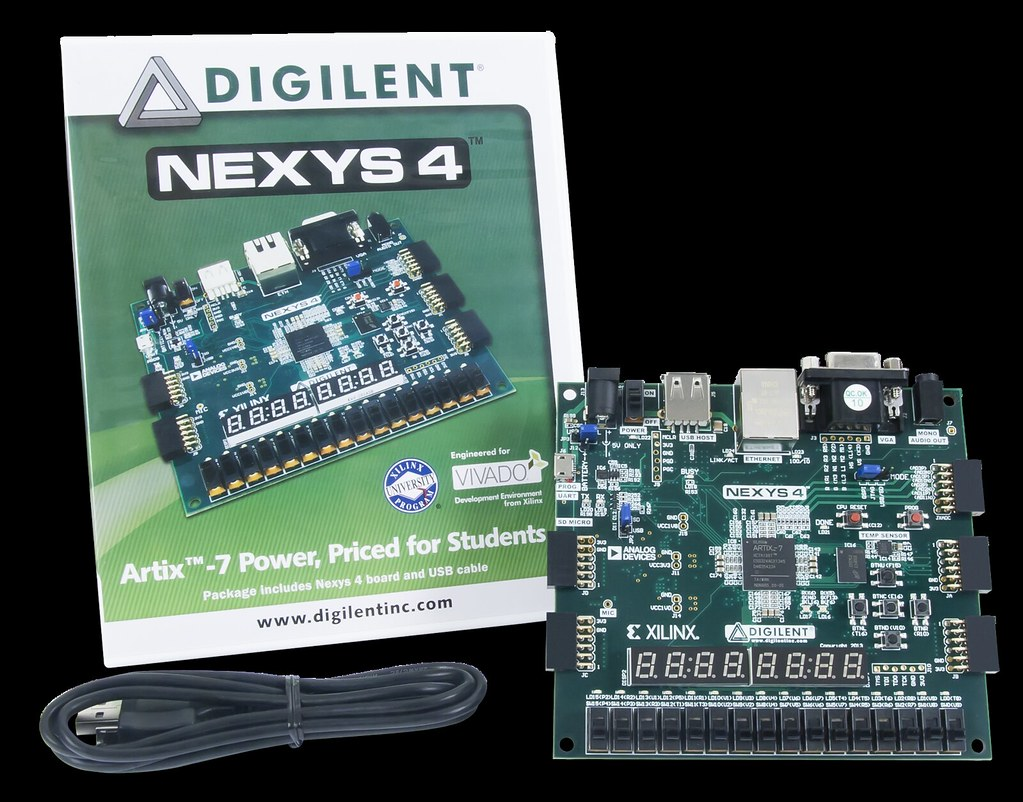
\includegraphics[width=0.4\linewidth]{images/img001_nexys4_board.jpg}
  \end{center}

  Documentation:

  \begin{itemize}
    \item \url{https://reference.digilentinc.com/reference/programmable-logic/nexys-4/reference-manual}
    \item \url{https://reference.digilentinc.com/\_media/reference/programmable-logic/nexys-4/nexys4\_rm.pdf}
  \end{itemize}
\end{minipage}

\begin{minipage}{\linewidth}
  \subsection{The Nexys4DDR board}

  No longer manufactured but still available for sale on some websites with old stock.

  \begin{center}
    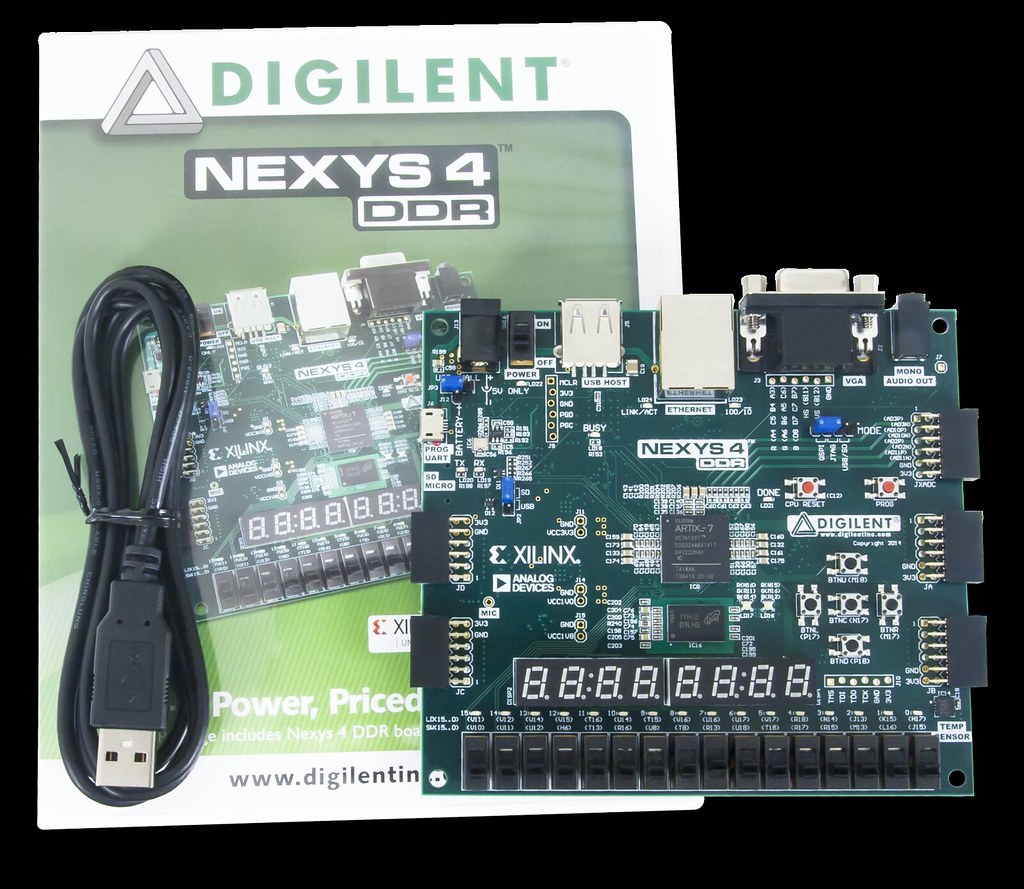
\includegraphics[width=0.4\linewidth]{images/img002_nexys4_ddr_board.jpg}
  \end{center}

  Documentation:

  \begin{itemize}
    \item \url{https://reference.digilentinc.com/reference/programmable-logic/nexys-4-ddr/reference-manual}
    \item \url{https://reference.digilentinc.com/\_media/reference/programmable-logic/nexys-4-ddr/nexys4ddr\_rm.pdf}
  \end{itemize}
\end{minipage}

\begin{minipage}{\linewidth}
  \subsection{The Nexys A7}

  This is the re-branded version of the above Nexys4 DDR board:

  \begin{center}
    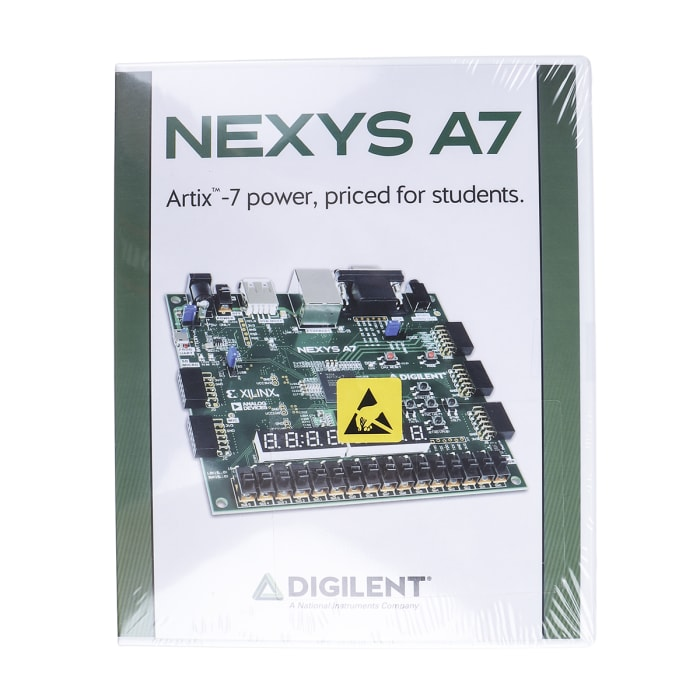
\includegraphics[width=0.4\linewidth]{images/img003_nexysA7_board.jpg}
  \end{center}

  Documentation:

  \begin{itemize}
    \item \url{https://reference.digilentinc.com/reference/programmable-logic/nexys-a7/reference-manual}
    \item \url{https://reference.digilentinc.com/\_media/reference/programmable-logic/nexys-a7/nexys-a7\_rm.pdf}
  \end{itemize}
\end{minipage}

\newpage

\section{Power, Jumpers, Switches and Buttons}

This top-down picture highlights the key jumper positions of interest on the Nexys4 board:

  \begin{center}
    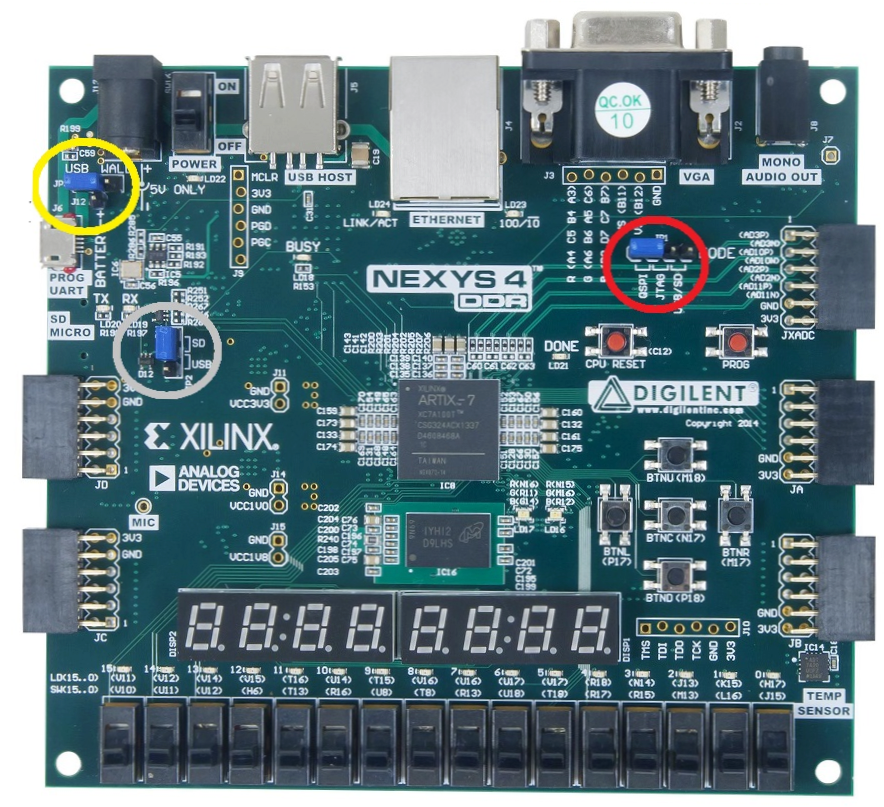
\includegraphics[width=0.9\linewidth]{images/nexys4_jumpers.png}
  \end{center}

The Nexys4 boards can be powered in two ways: using an external power supply, or from a standard USB port.

\subsection{Micro-USB Power}

\includegraphics[width=5cm]{images/illustrations/nexys-micro-usb-power.pdf}

Connect your micro-usb cable to a USB port on a USB charger or PC to provide power. Connect the other end to the Nexys4's micro-usb connector. Place the JP3 jumper on pins 1 and 2 to select USB power. Use the switch to power up the Nexys4.

\subsection{External Power Supply}

\hspace*{1.7cm}
\includegraphics[width=3.2cm]{images/illustrations/nexys-power-supply.pdf}

The MEGA65 core can consume a lot of power, and a standard USB port could potentionally be too little for the Nexys4 board. In particular, writing to the SD card might hang or perform odd behaviour. Therefore you should consider a 5V power supply.

Digilent sell a power supply for the Nexys4 board, and we recommend you use this to ensure you avoid the risk of damage to your Nexys4 board. The chosen power supply should be center positive, 2.1mm internal diameter plug, and should deliver 4.5VDC to 5.5VDC rated at least 1 Amp.

Connect the power supply cable to the supply plug of the Nexys4. Place the JP3 jumper on pins 2 and 3 to select WALL power. Use the switch to power up the Nexys4.

\subsection{Other Jumpers and Switches}

For your initial set up, we'd suggest you set the following jumpers on your Nexys4 board to these positions:

\begin{itemize}
  \item{JP1} - USB/SD
  \item{JP2} - SD
\end{itemize}

\begin{center}
  \includegraphics[width=3.2cm]{images/illustrations/nexys-jumpers.pdf}
\end{center}

This will assure that the bitstream files will get loaded from your SD card on start-up.

At some later stage, you may prefer to load the bitstream from the on-board QSPI flash, and at that point, you can revisit your JP1 jumper setting and adjust it to the QSPI position.

% XXX - Image of board highlighting the jumpers

All 16 switches on the lower edge of the board must be set to the off position.


\subsection{Connections and Peripherals}

\includegraphics[width=\linewidth]{images/illustrations/nexys-connectors.pdf}

A USB keyboard can be connected to the USB port. Only a keyboard that lacks a USB hub will work with the Nexys4 board.  Generally, extremely cheap keyboards will work, while more expensive keyboards tend to have a USB hub integrated, and will not work.  You may need to try several keyboards before you find one that works.

You can connect a VGA monitor to the VGA port.

The mono audio-out jack can be connected to the line-in of an amplifier.


\subsection{Communicating with your PC}

There may be occasions where you wish to communicate with your Nexys4 board from your PC, in order to perform activities such as:

\begin{itemize}
  \item Flash your QSPI flash chip via Vivado
  \item Upload bitstream files directly from your PC (via m65 tool)
  \item Make use of support tools such as M65Connect, m65, mega65\_ftp, m65dbg, etc
\end{itemize}

On such occasions, you will need to connect your micro-usb cable up to your PC.

\includegraphics[width=5cm]{images/illustrations/nexys-micro-usb-power.pdf}

\subsection{Onboard buttons}

\begin{center}
  \includegraphics[width=3.2cm]{images/illustrations/nexys-reset-buttons.pdf}
\end{center}

The ``CPU RESET'' button will reset the MEGA65 when pressed, while the ``PROG'' button will cause the FPGA itself to reload the MEGA65
core.  The main difference between the two is that CPU RESET is faster, and does not clear the contents of memory, while the FPGA button
is slower, and does reset the contents of memory.

\begin{center}
  \includegraphics[width=3.2cm]{images/illustrations/nexys-five-buttons.pdf}
\end{center}

Two of the five buttons in the cross arrangement can also be used:  BTND acts as though you have pressed the \widekey{RESTORE} key, while BTNC will trigger an IRQ, as though the IRQ line had been pulled to ground.

\section{Keyboard}

The keyboard layout is positional rather than logical.
This means that keys in similar positions to the keys on a C65 keyboard will have similar function.
This relationship assumes that your USB keyboard uses a US keyboard layout.

To help you locate what the various MEGA65 keys are mapped to, the MEGA65 has a built-in virtual keyboard test feature. This can be accessed in two ways.

The easiest way is to keep the \specialkey{ALT} key held in while turning on the Nexys4, or resetting the Nexys4 with the ``PROG'' button. The configure menu will be presented and by pressing 3, the virtual keyboard will be presented on a black background.

\includegraphics[width=\linewidth]{images/illustrations/virtual-keyboard.pdf}

Pressing a key on the USB keyboard will show the highlighted key on the virtual keyboard to help you identify the key mapping.

The other way to access the virtual keyboard is from within the MEGA65. Hold \megasymbolkey and press \megakey{TAB} to access the Matrix Mode Debugger. From here, enter the following:

\screentextwide{s ffd3615 ff}

This will open a semi-transparent virtual keyboard at the top of the screen. Alternatively:

\screentextwide{s ffd3615 ff ff}

This will open a semi-transparent virtual keyboard in the centre of the screen.

Hold \megasymbolkey and press \megakey{TAB} to exit Matrix Mode Debugger and return to the MEGA65.

\subsection{Some key mappings with a USB keyboard}

The \widekey{RESTORE} key is mapped to the PAGE UP key.

The \specialkey{RUN STOP}  key is mapped to the ESC key.

\newpage

\section{Preparing microSDHC card}

The MEGA65 requires an SDHC card of between 4GB and 64GB capacity.  Some SDXC cards may work, however, this is not officially supported.

Preparation steps for the Nexys4 board's SD card share much in common with the steps needed for real MEGA65 hardware, and as such, it is worth having a look over the \nameref{cha:configuring} chapter if you ever need details.

So in this section, we'll provide more details on the distinctive steps, and be more brief on the common steps.

One point of distinction between the Nexys board and the real MEGA65 hardware is that the latter already has a default bitstream/core provided, which permits you to format your SD card in the specific style required by the MEGA65.

For Nexys4 board owners however, you have no such default bitstream, so
see \nameref{sec:bitstreamfiles} for more details on where the appropriate "nexys4.bit" or "nexys4ddr-widget.bit" files for your device can be downloaded from.

\subsection{Preparation Steps}

The steps are:

\begin{itemize}
  \item{Format the SD card} in a convenient computer using the FAT32 file-system.  The MEGA65 and Nexys4 boards do not understand other
file systems, especially the exFAT file system.
\item{Copy} your bitstream file (with name ending in ``.bit'') onto the SD card.
\item{Insert} the SD card into the SD card slot on the under-side of the Nexys4 board.
\item{Switch on} the Nexys4 board.
\item{Enter the Utility Menu} by holding the \specialkey{ALT} key down on the USB keyboard you have connected to the Nexys4 board.
\item{Enter the FDISK/FORMAT tool} by pressing 2 when the option appears on the MEGA65 boot screen.
\item{Follow the prompts} in the FDISK/FORMAT program to again format the SD card for use by the MEGA65. \\
  \\
  The FDISK tool will partition your SD card into two partitions and format them.
  \begin{itemize}
    \item One is type \$41 = MEGA65 System Partition, where the save slots, configuration data and other files live. \\
  (This partition is invisible in i.e. Win PCs).
    \item The other partition with type \$0C = VFAT32, where KERNEL, support files, games, and so on, will be copied to later. \\
  (This partition is visible on i.e. Win PCs).
  \end{itemize}
\item{Once formatting is complete}, switch off the Nexys4 board and remove the microSDHC card from the Nexys board and put it back into your PC
\item{This time, copy} the following items onto the SD card:
  \begin{itemize}
    \item The bitstream file
    \item The extracted files from within either the "\textbf{SD essentials.rar}" or "\textbf{SD essentialsNoROM.rar}" file that you downloaded from the MEGA65 filehost. (See \nameref{sec:installingrometc} for more details).
    \item{If you have sourced your own preferred ROM file} (e.g. "\textbf{911001.BIN}"), copy it onto the SD card also, and rename it to "\textbf{MEGA65.ROM}" (uppercase is essential).
    \item{Any .D81 disk image files} you wish to make use of.
      \begin{itemize}
        \item Note that if a file named MEGA65.D81 is added to the SD card, it will be mounted automatically on startup.
        \item Make sure that all .D81 files have names that fit the old DOS 8.3 character limit, and are upper case.  This restriction will be removed in a future release.
      \end{itemize}
  \end{itemize}
\item{Remove the SD card} and reinsert it into your Nexys4 board.
\item{Power the Nexys4} board back on.  The MEGA65 should boot within 15 seconds.
\item On first start up, you will find yourself at the on-boarding screen, of which more details can be found in the \nameref{cha:configuring} chapter.

\end{itemize}

Congratulations. Your MEGA65 has been set up and is ready to use.

Please note that the above method of copying the bitstream file to the SD card means that the bitstream is loaded into the Nexys FPGA each time on boot - which takes around 13 seconds for the system to start. The bitstream can also be flashed using Vivado software into the QSPI flash to deliver a boot up time of 0.3 seconds. 

For more detailed information on preparing and configuring your MEGA65, please refer to the \nameref{cha:configuring} chapter. 

\section{Loading the bitstream from QSPI}

While loading the bitstream from the SD card is the suggested (and well-trodden) path this document has chosen, of late, more nexys4 users have been exploring the alternative pathway of loading the bitstream from the QSPI flash. Some potential reasons they have chosen this pathway are:

\begin{itemize}
  \item Faster loading times (0.3 seconds versus 13 seconds)
  \item Some people were interested in the possibility of flashing multiple cores onto their QSPI (via steps described in the \nameref{cha:cores} Chapter)
  \item Some people have experienced niggling issues with the SD card pathway, such as:
    \begin{itemize}
      \item System unable to reboot from on-boarding screen
      \item System unable to reboot from freeze-menu after switching between PAL/NTSC
    \end{itemize}
\end{itemize}

In time, if this proves to be a more popular pathway, we can revise our documentation here to suit it. Here are some steps in brief.

\subsection{Preparation Steps}

For users that want to try this pathway, you will need to adjust the JP1 jumper setting to use QSPI and then follow the steps in the \nameref{cha:fpgacpldflashing} chapter in relation to \nameref{sec:installvivado} and \nameref{sec:mainfpgaflashing}.

Be forewarned that the installation of Vivado is a lengthy process (both in terms of download time, and installation time).

Once you have flashed Slot0 of your QSPI chip via Vivado, you can then follow the steps described in \nameref{cha:configuring} to perform the custom SD card formatting, installing of ROM and support files and on-boarding.

\section{Useful Tips}

The following are some useful tips for getting familiar with the MEGA65:

\begin{itemize}

\item{Press \& hold \megasymbolkey (or the Commodore key if using a Commodore 64 or 65 keyboard) during boot to start up in C64 mode instead of C65 mode}
 \item{Press \& hold \specialkey{RUN STOP} during boot to enter the machine language monitor, instead of starting BASIC.}
\item{Press the \widekey{RESTORE} key for approximately 1/2 - 1 second to enter the MEGA65 Freeze Menu.  From this menu
  you have convenient tools to change the CPU speed, switch between PAL \& NTSC video mode, change Audio settings, manage freeze-states,
   select D81 disk images, examine and modify memory of the frozen program, among other features.  This is in many ways the heart of the MEGA65, so it is well worth exploring and getting familiar with.}
\item{Type \screentext{POKE0,65} in C64 mode to switch  the CPU to full speed (40MHz). Some software may behave incorrectly in this mode, while other software will work very well, and run many times faster than on a C64.}
\item{Type \screentext{POKE0,64} in C64 mode to switch the CPU to 1MHz.}
\item{Type \screentext{SYS58552} in C64 mode to switch to C65 mode.}
\item{Type \screentext{GO64} in C65 mode and confirm, by pressing \screentext{Y}, to switch to C64 mode, just like on a C128.}
\item{The C65 ROM makes device 8 the default, so you can normally leave off the \textbf{,8} from the end of LOAD and SAVE commands.}
\item{Pressing \specialkey{SHIFT} + \specialkey{RUN STOP} from either C64 or C65 mode will attempt to boot from disk.}
\end{itemize}

Have fun! The MEGA65 has been lovingly crafted over many years for your enjoyment. We hope you have as much fun using it as we have had creating it!

The MEGA Museum of Electronic Games \& Art welcomes your feedback, suggestions and contributions to this open-source digital heritage preservation project.


\part{APPENDICES}

\appendix
  \chapter{Flashing the FPGAs and CPLDs in the MEGA65}
\label{cha:fpgacpldflashing}

The MEGA65 is an open-source and open-hardware computer. This means you are free,
not only to write programs that run on the MEGA65 as a finished computer, but also to
use the re-programmable chips in the MEGA65 to turn it into all sorts of other things.

If you just want to install an upgrade core for the MEGA65, or a core that lets you use
your MEGA65 as another type of computer, you are probably want to look in
\bookvref{cha:cores} instead.
This chapter is more intended for people who want to help develop cores for the MEGA65.

These re-programmable chips are called Field Programmable Gate Arrays (FPGAs) or
Complex Programmable Logic Devices (CPLDs), and can implement a wide variety of circuits.
They are normally programmed using a language like VHDL or Verilog.  These
are languages that are not commonly encountered by most people.  They are also quite
different in some ways to ``normal'' programming languages, and it can take a while to
understand how they work. But with some effort and perseverance, exciting things can be created with them.

Be prepared to install many gigabytes of software on a Linux or Windows PC, before you will
be able to write programs for the FPGAs and CPLDs in the MEGA65.  Also,
"compiling" complex
designs can take up to several hours, depending on the speed and memory
capacity of your computer.
We recommend a computer with at least 8GB RAM (preferably 16GB) if you want to write
programs for FPGAs and CPLDs. On the other hand, if all you want to do is load programs onto
your MEGA65's FPGAs and CPLDs that other people have written, then most
computers running a recent
version of Windows or Linux should be able to cope.

\section{Warning}

Before we go any further, we do have to provide a warning about reprogramming the FPGAs and
CPLDs in the MEGA65.
Re-programming the MEGA65 FPGA can potentially cause
damage, or leave your MEGA65 in an unresponsive state from which it is very difficult to
recover, i.e., ``bricked''.  Therefore if you choose to open your MEGA65 and reprogram
any of the FPGAs it contains, it is no longer possible to guarantee its correct operation.
Therefore, we cannot reasonably honour the warranty of the
device as a computer.
You have been warned!

\section{Installing Vivado}
\label{sec:installvivado}

Installation of Vivado is required to flash the QSPI flash memory within your MEGA65 target device, whether it be a MEGA65 R2/R3, Nexys4/Nexys4DDr/NexysA7, MEGAphone or other.

Vivado is also the tool used to perform compilation (synthesis, as it is preferably called) of FPGA bitstreams.

To get started, connect to \url{https://www.xilinx.com/support/download.html}

\begin{minipage}{\linewidth}
  Select 2020.2 version
  \\
  \begin{center}
    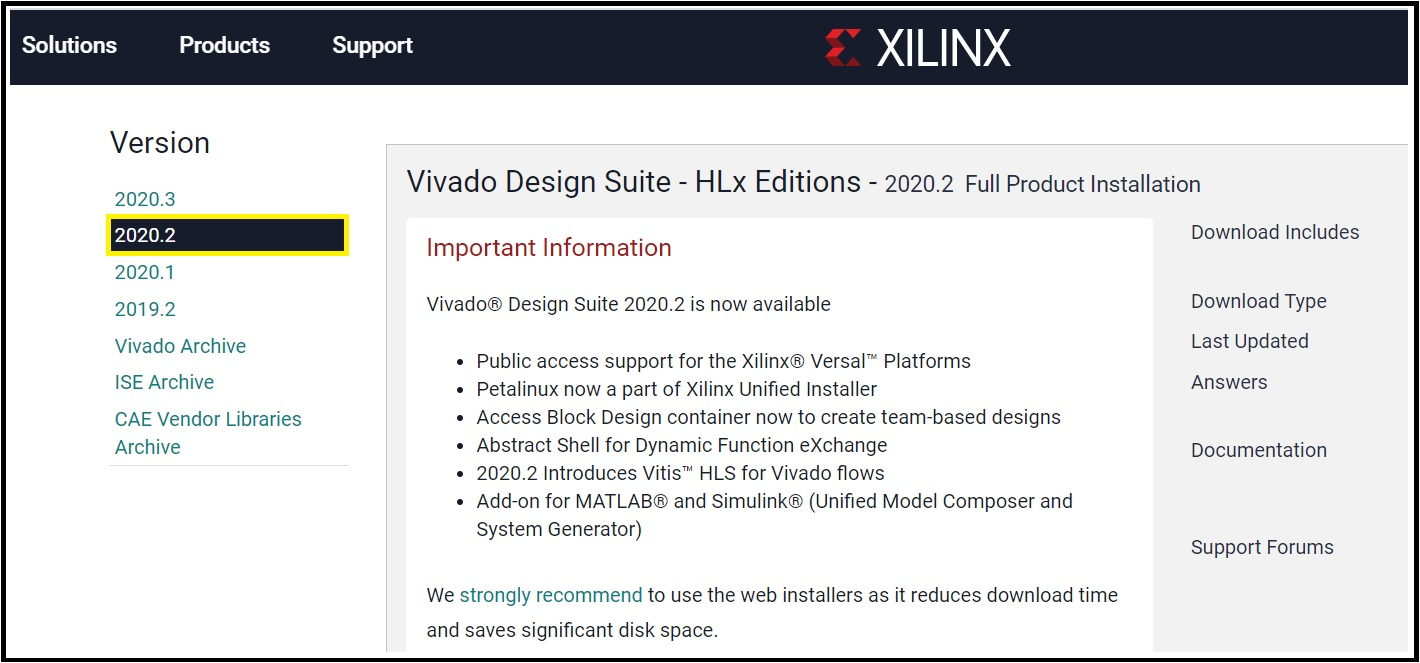
\includegraphics[width=\linewidth]{images/VivadoInstimg002.jpg}
  \end{center}
  NOTE : Some users still have success with using older versions, as the main aim here is to install a version that supports the FPGA of your target hardware. \\
  \\
  I.e., the Artix7 100T (for Nexys and R2) or 200T (R3).
\end{minipage}

\begin{minipage}{\linewidth}
  Click on Xilinx Unified Installer 2020.2: Windows Self Extracting Web Installer EXE - 248.44 MB 
  \\
  \begin{center}
    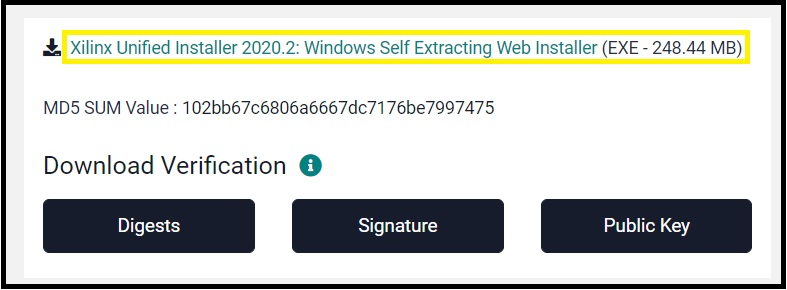
\includegraphics[width=0.8\linewidth]{images/VivadoInstimg003.jpg}
  \end{center}
\end{minipage}

\begin{minipage}{\linewidth}
  You will be asked to create an account in order to sign in and be able to download the installation program. \\
  \\
  Your credentials will also be requested when doing the installation.
  \\
  \begin{center}
    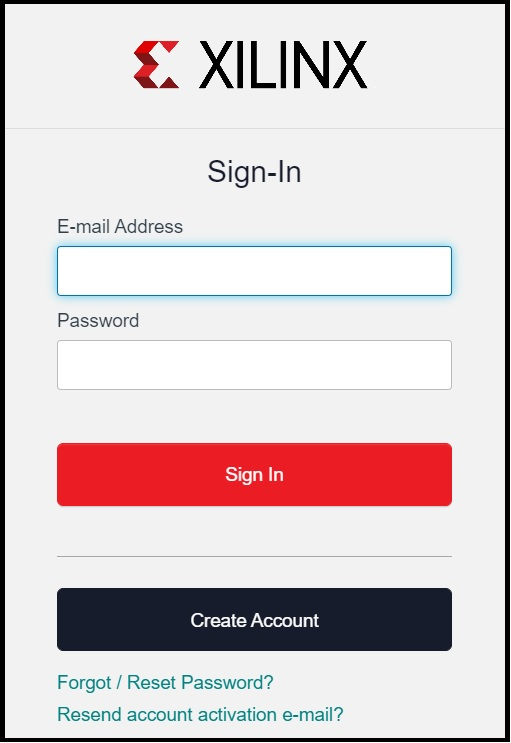
\includegraphics[width=0.3\linewidth]{images/VivadoInstimg004.jpg}
  \end{center}
\end{minipage}

\begin{minipage}{\linewidth}
  After having signed in, you have to provide some personal information and then click on Download
  \\
  \begin{center}
    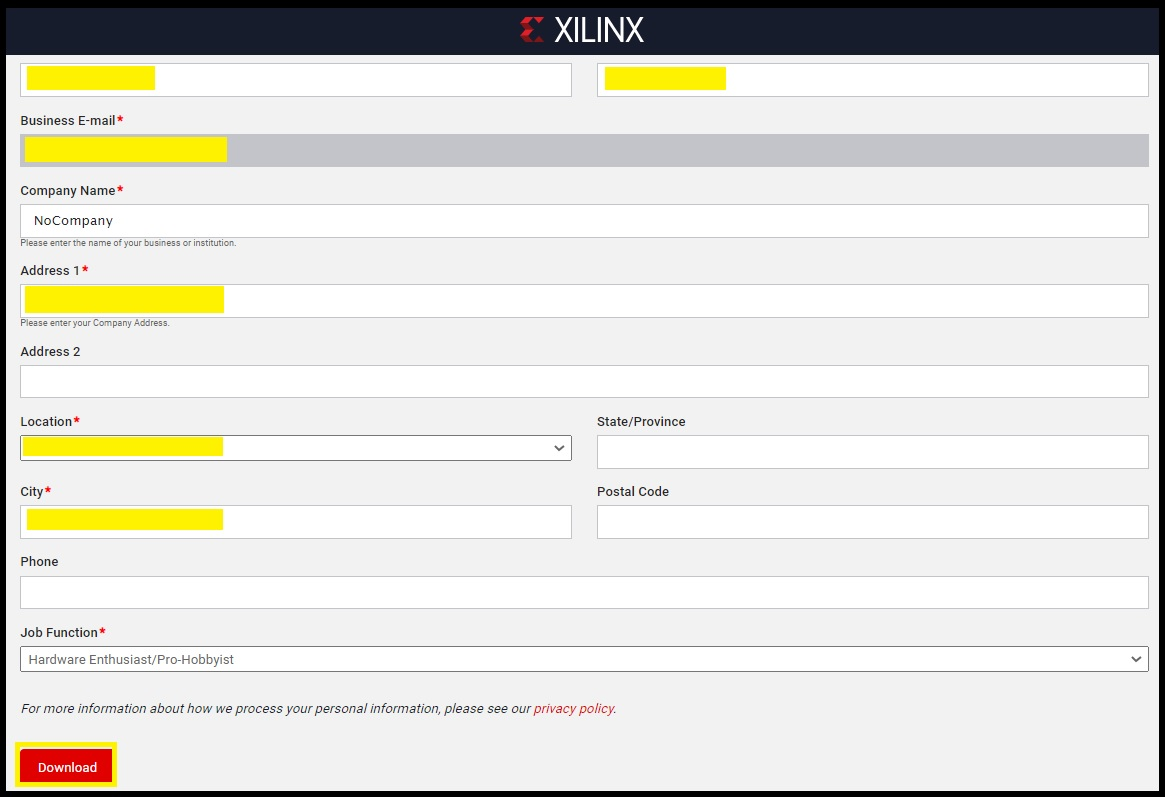
\includegraphics[width=0.8\linewidth]{images/VivadoInstimg005.jpg}
  \end{center}
\end{minipage}

\begin{minipage}{\linewidth}
  Execute the installer as Administrator (Xilinx\_Unified\_2020.2\_1118\_1232\_Win64.exe).
  \\
  \begin{center}
    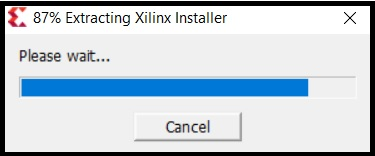
\includegraphics[width=0.5\linewidth]{images/VivadoInstimg006.jpg}
  \end{center}
\end{minipage}

\begin{minipage}{\linewidth}
  Click on Allow Access.
  \\
  \begin{center}
    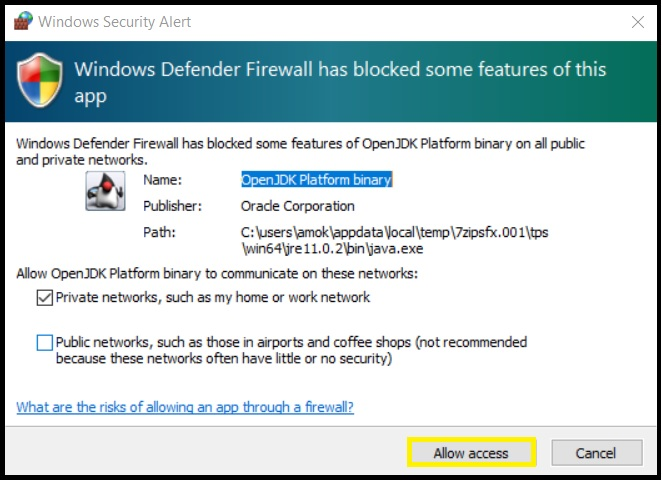
\includegraphics[width=0.5\linewidth]{images/VivadoInstimg007.jpg}
  \end{center}
\end{minipage}

\begin{minipage}{\linewidth}
  Click on Next.
  \\
  \begin{center}
    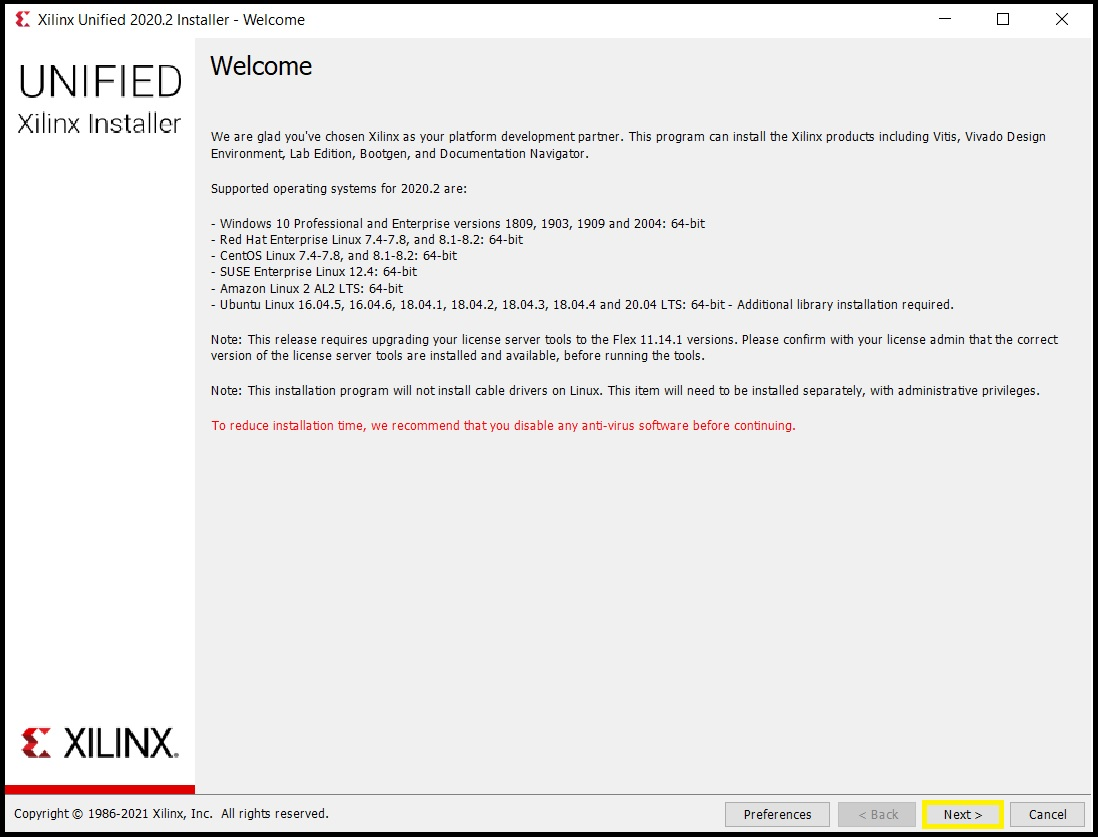
\includegraphics[width=0.7\linewidth]{images/VivadoInstimg008.jpg}
  \end{center}
\end{minipage}

\begin{minipage}{\linewidth}
  Enter your credentials and click on Next.
  \\
  \begin{center}
    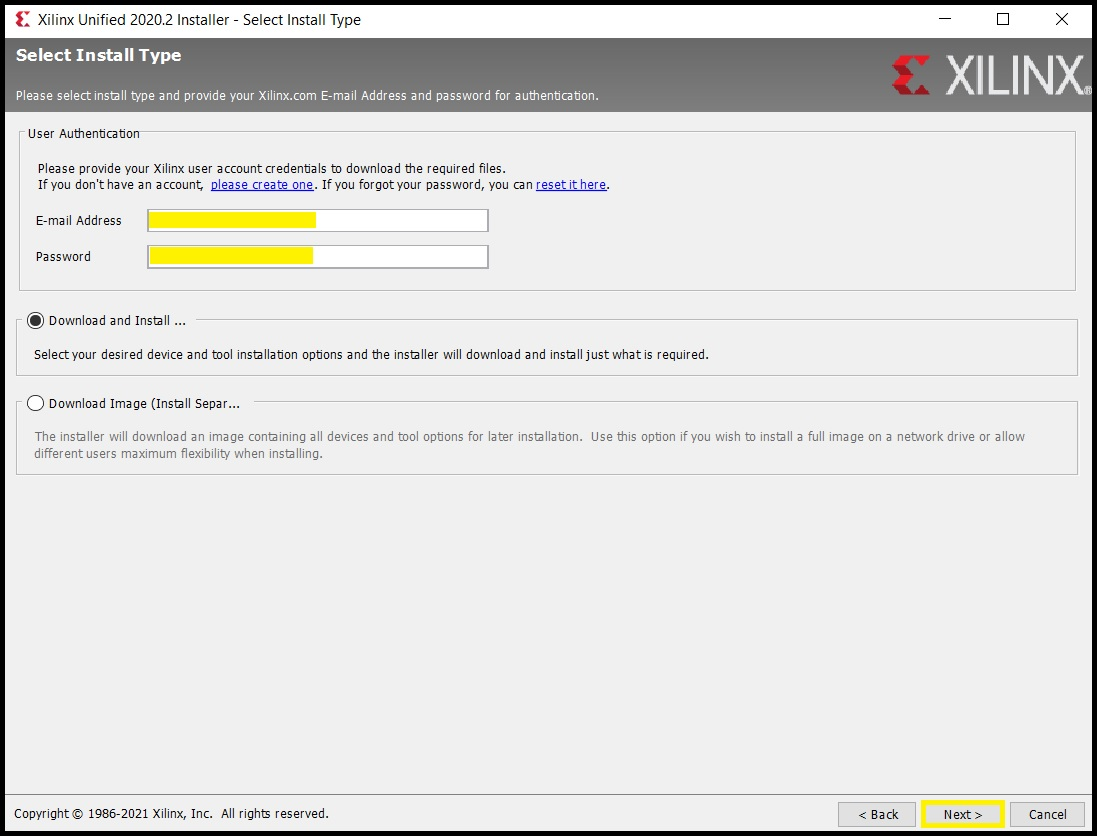
\includegraphics[width=0.7\linewidth]{images/VivadoInstimg009.jpg}
  \end{center}
\end{minipage}

\begin{minipage}{\linewidth}
  Select Vivado and click on Next.
  \\
  \begin{center}
    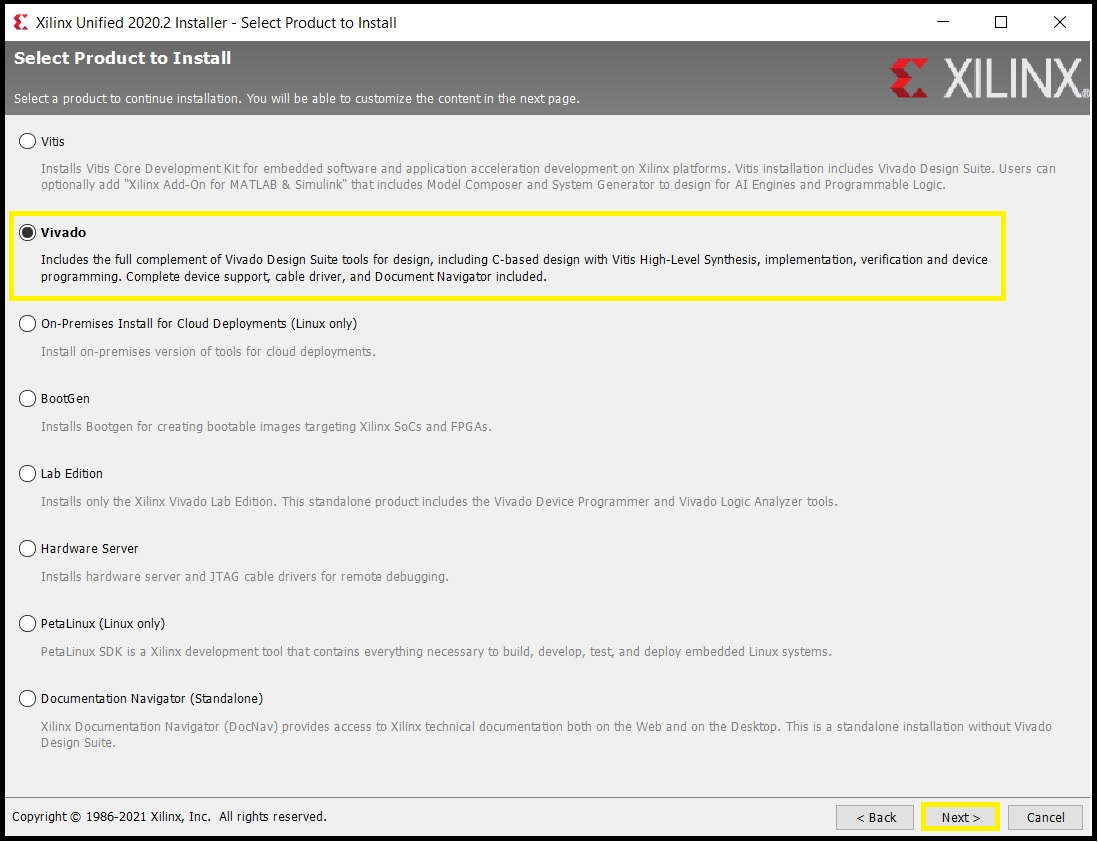
\includegraphics[width=0.7\linewidth]{images/VivadoInstimg010.jpg}
  \end{center}
\end{minipage}

\begin{minipage}{\linewidth}
  Select "Vivado HL WebPACK" and click on "Next"
  \\
  \begin{center}
    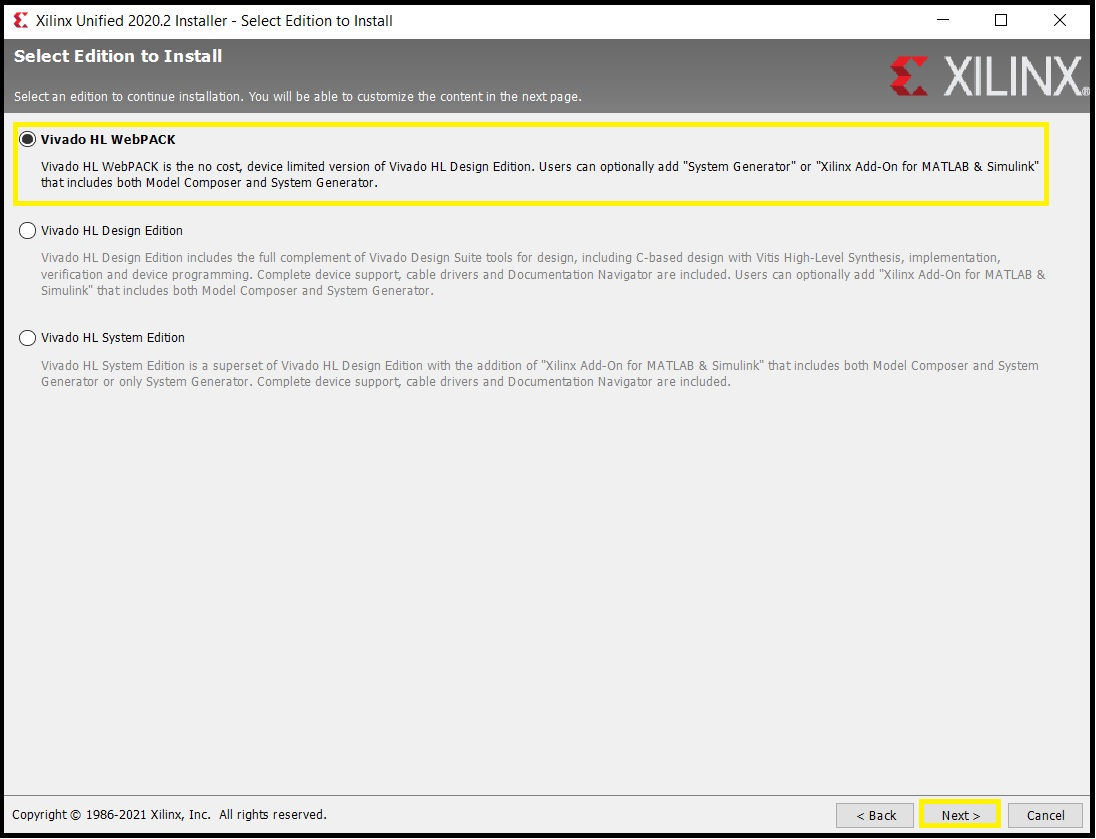
\includegraphics[width=0.7\linewidth]{images/VivadoInstimg011.jpg}
  \end{center}
\end{minipage}

\begin{minipage}{\linewidth}
  Keep the default selection and click on "Next"
  \\
  \begin{center}
    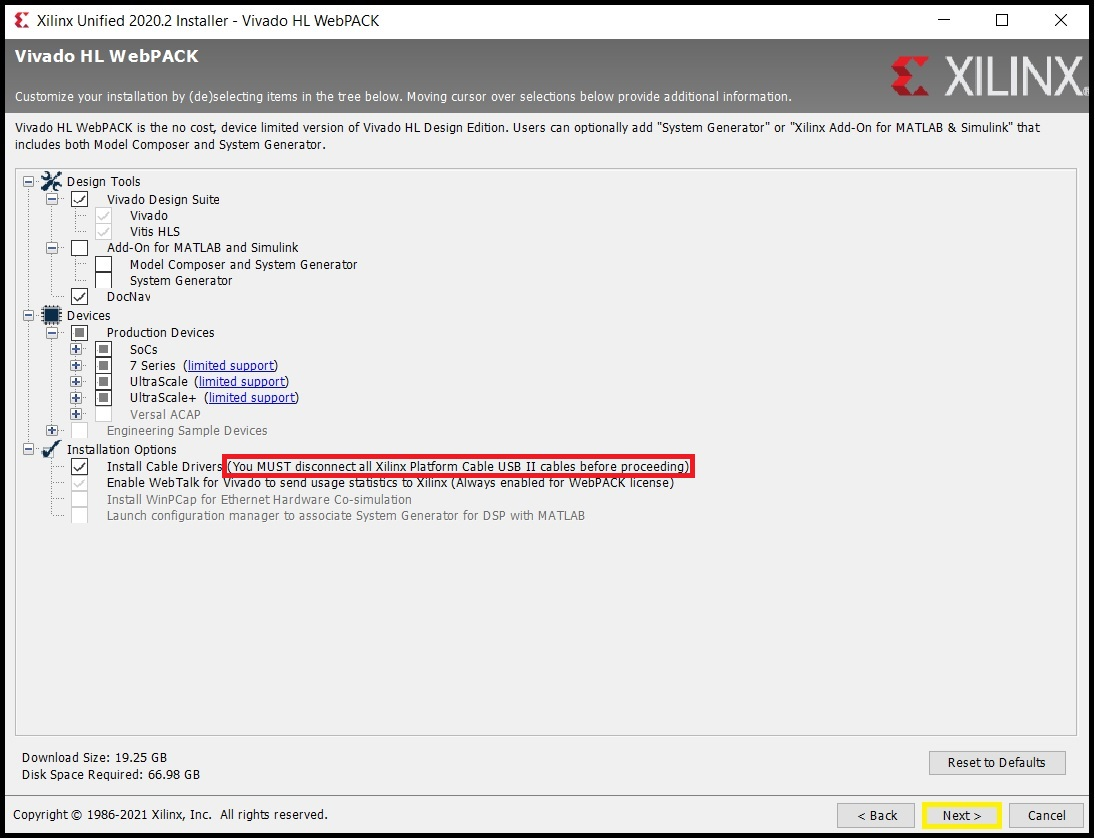
\includegraphics[width=0.7\linewidth]{images/VivadoInstimg012.jpg}
  \end{center}
  Warning: As stated, disconnect any USB cable that would be connected to your PC from the Nexys board.
\end{minipage}

\begin{minipage}{\linewidth}
  Agree with all the End User Licence Agreement and Terms and conditions and click on "Next".
  \\
  \begin{center}
    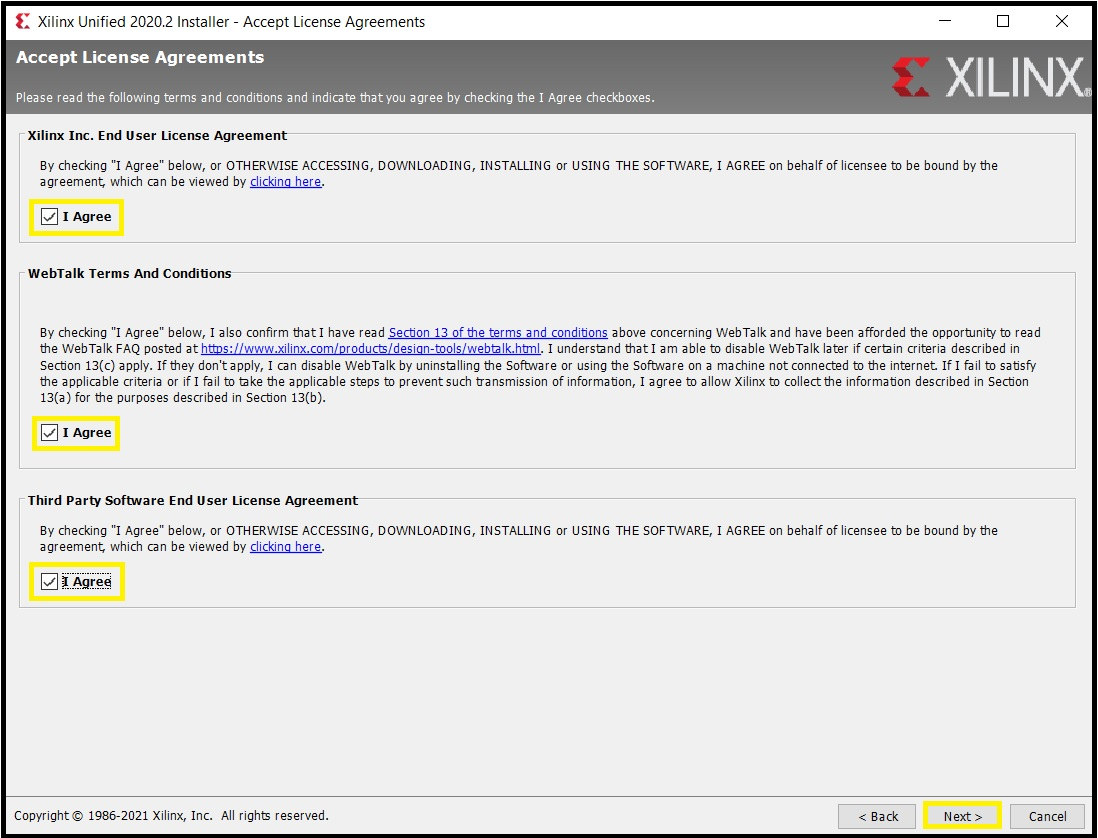
\includegraphics[width=0.7\linewidth]{images/VivadoInstimg013.jpg}
  \end{center}
\end{minipage}

\begin{minipage}{\linewidth}
  Choose the location where you want to install the software and click on "Next".
  \\
  \begin{center}
    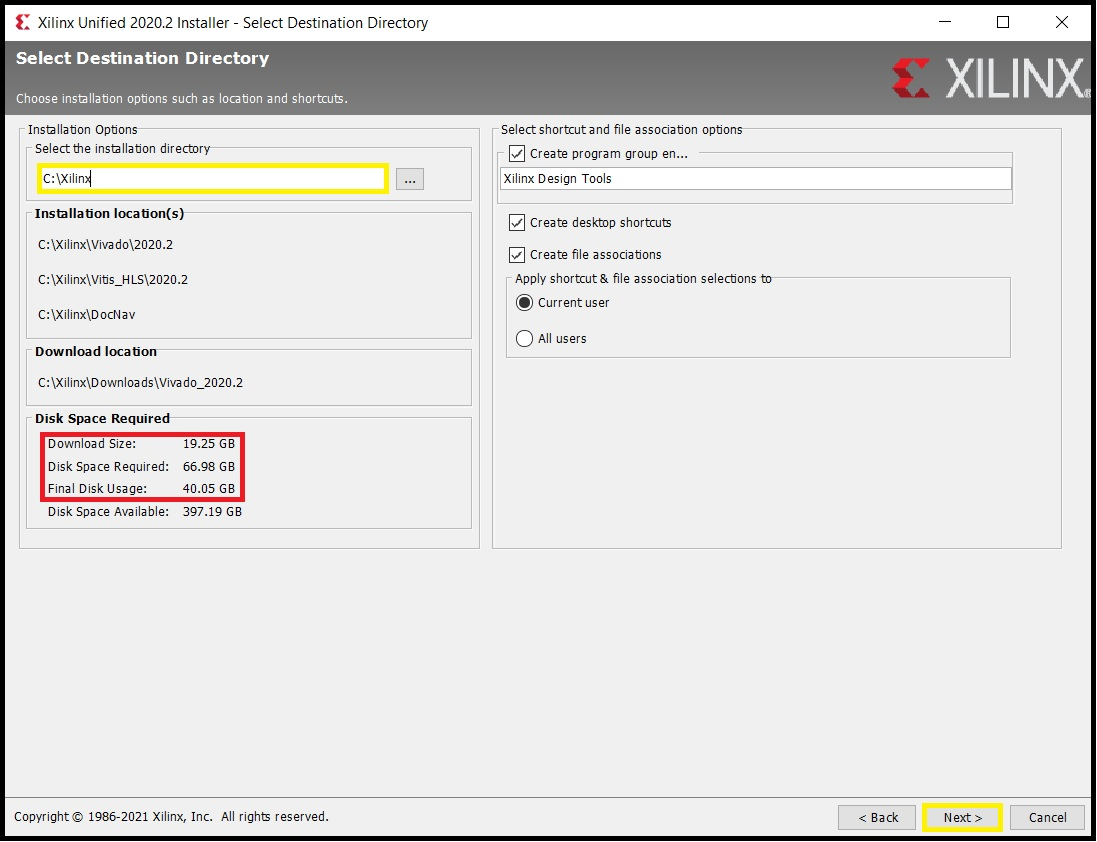
\includegraphics[width=0.7\linewidth]{images/VivadoInstimg014.jpg}
  \end{center}
  Warning : You are about to download 20GB of software and you need 70GB to perform the installation.
\end{minipage}

\begin{minipage}{\linewidth}
  Click on "Yes"
  \\
  \begin{center}
    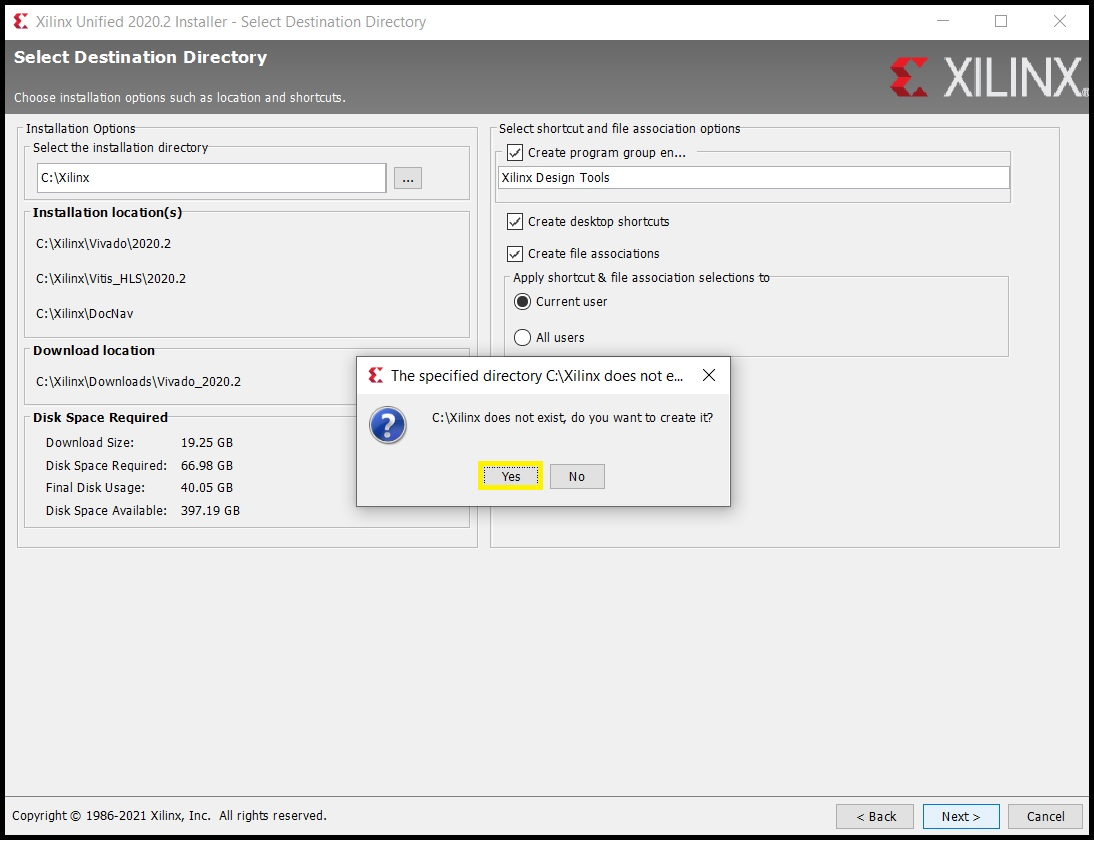
\includegraphics[width=0.7\linewidth]{images/VivadoInstimg015.jpg}
  \end{center}
\end{minipage}

\begin{minipage}{\linewidth}
  Click on "Install"
  \\
  \begin{center}
    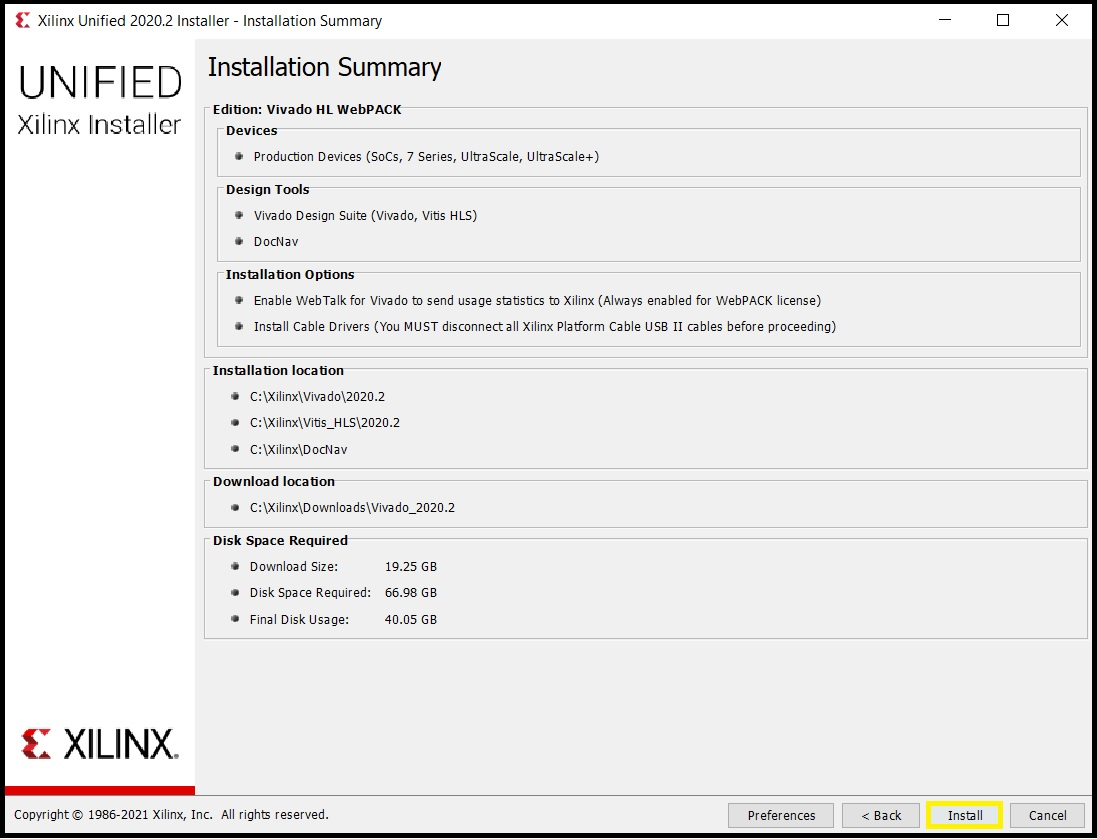
\includegraphics[width=0.7\linewidth]{images/VivadoInstimg016.jpg}
  \end{center}
\end{minipage}

\begin{minipage}{\linewidth}
  Wait for the installation to complete. At the very end of the installation you will be asked if you want
  to install Xilinx device software.
  \\
  \begin{center}
    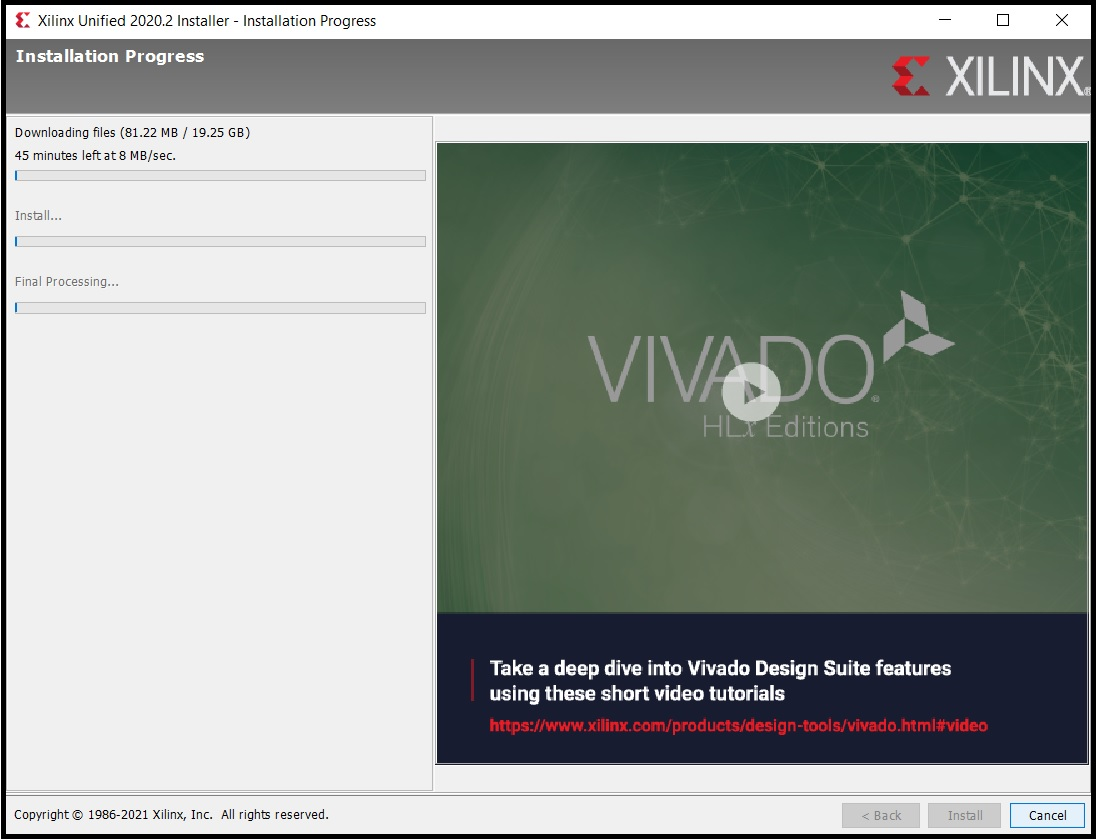
\includegraphics[width=0.7\linewidth]{images/VivadoInstimg017.jpg}
  \end{center}  
\end{minipage}

\begin{minipage}{\linewidth}
  Click on "Install"
  \\
  \begin{center}
    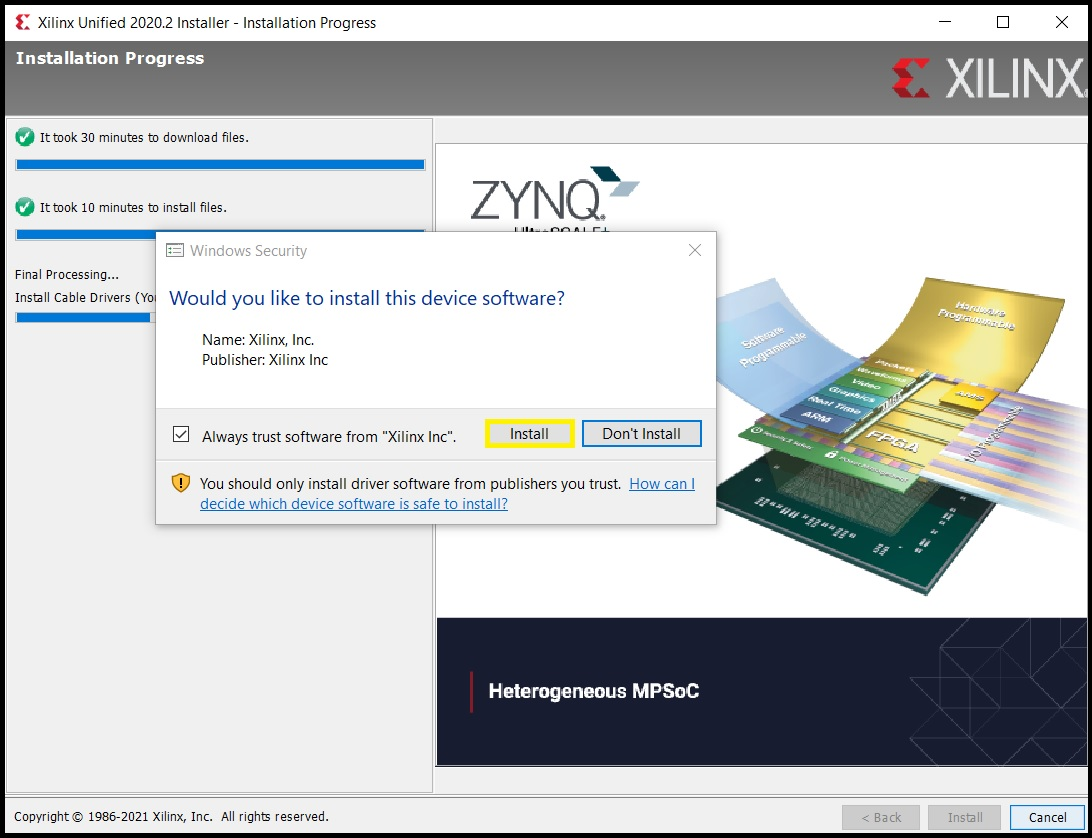
\includegraphics[width=0.7\linewidth]{images/VivadoInstimg018.jpg}
  \end{center}
  Let the installation complete.
\end{minipage}

\begin{minipage}{\linewidth}
  The installation is completed. Click on "OK"
  \\
  \begin{center}
    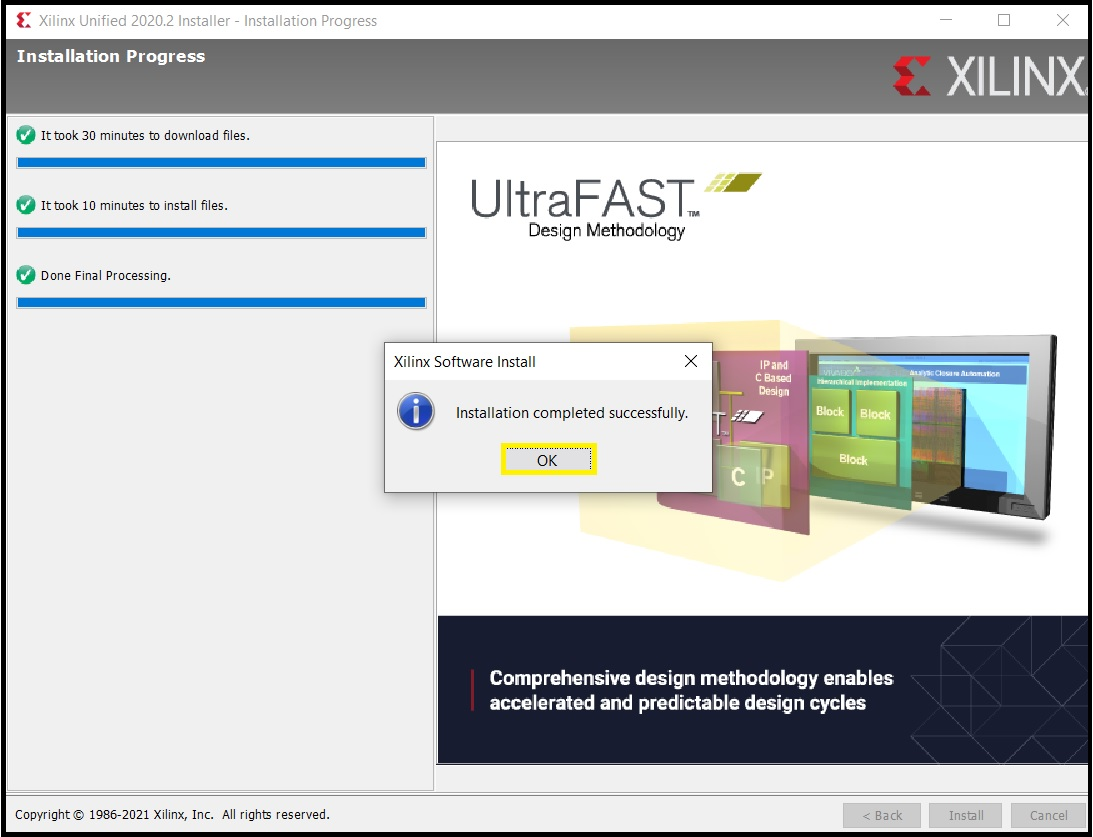
\includegraphics[width=0.7\linewidth]{images/VivadoInstimg019.jpg}
  \end{center}
\end{minipage}

\begin{minipage}{\linewidth}
  You end up with the following icons on your desktop:
  \\
  \begin{center}
    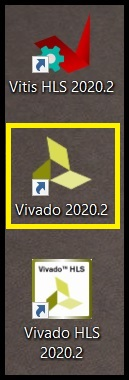
\includegraphics[width=0.2\linewidth]{images/VivadoInstimg020.jpg}
  \end{center}
\end{minipage}

\begin{minipage}{\linewidth}
  Launch Vivado 2020.2
  \\
  \begin{center}
    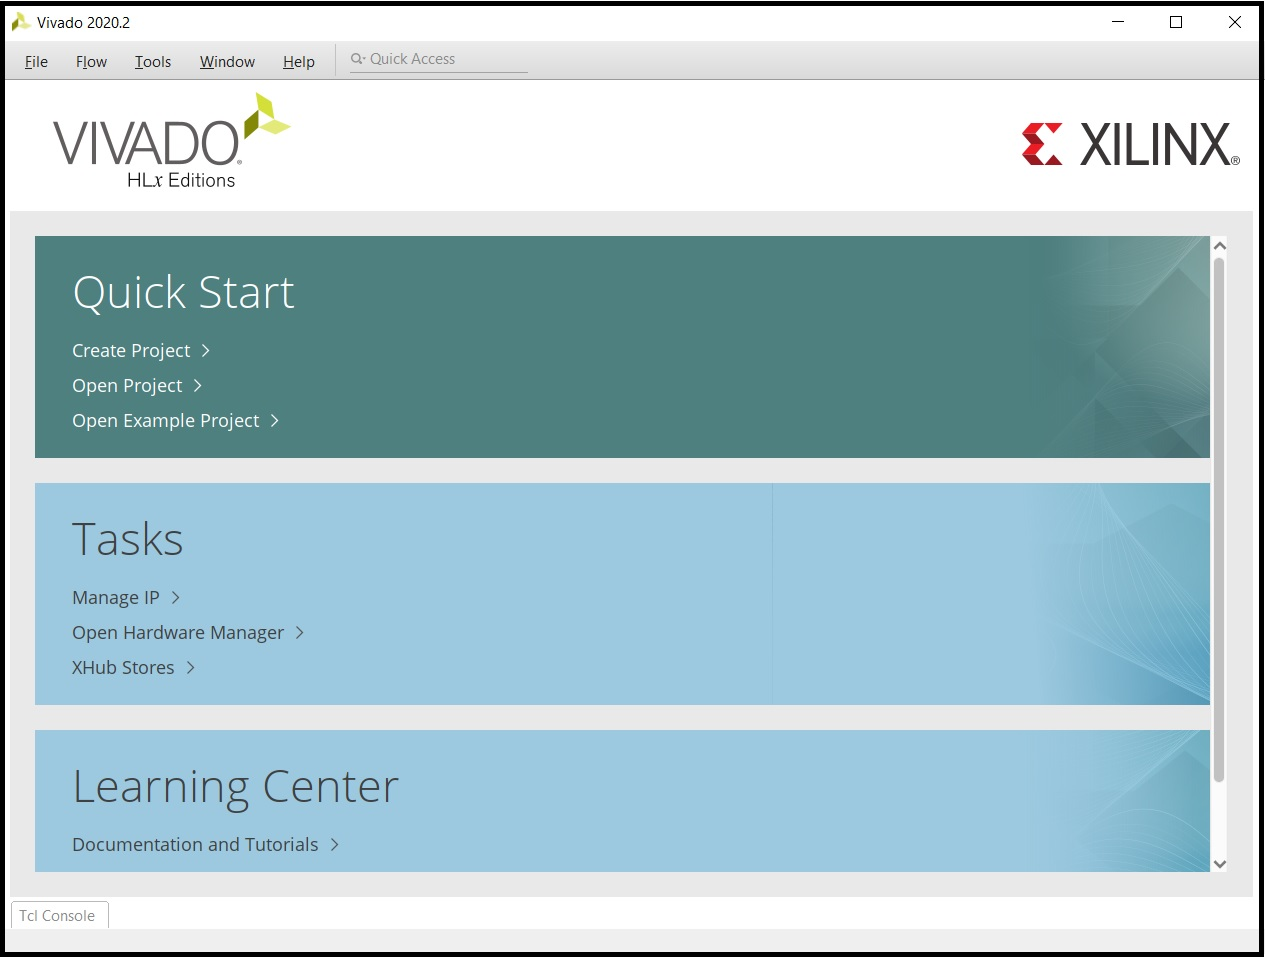
\includegraphics[width=0.7\linewidth]{images/VivadoInstimg021.jpg}
  \end{center}
\end{minipage}

\begin{minipage}{\linewidth}
  Click on "Help"->"Obtain a licence Key"
  \\
  \begin{center}
    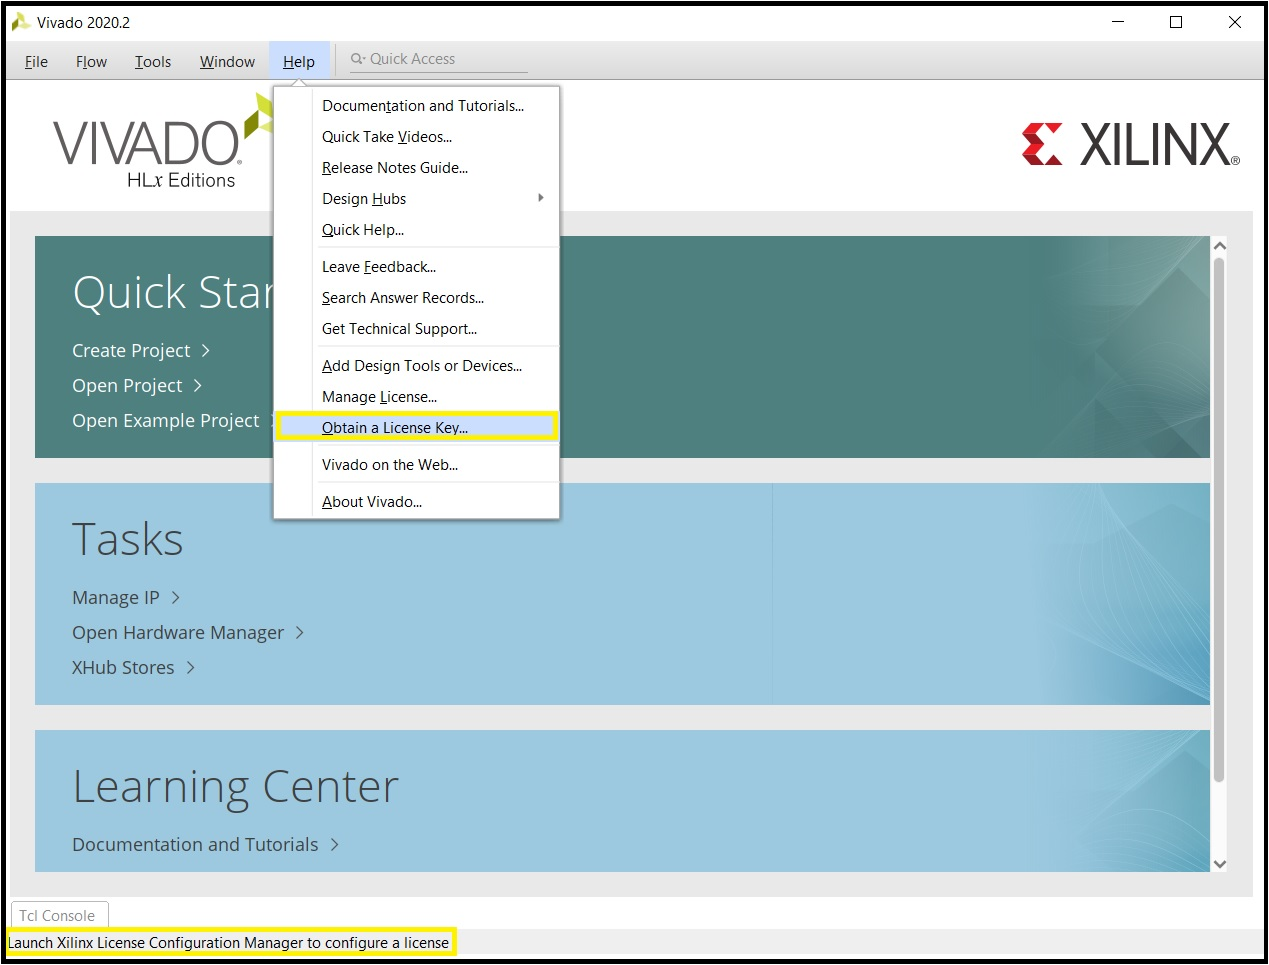
\includegraphics[width=0.7\linewidth]{images/VivadoInstimg022.jpg}
  \end{center}
\end{minipage}

\begin{minipage}{\linewidth}
This launches the Vivado licence manager \\
  \\
  Select "Get Free ISE WebPACK, ISE/Vivado IP or PetaLinux Licenses" \\
  \\
  Click on "Connect Now"
  \\
  \begin{center}
    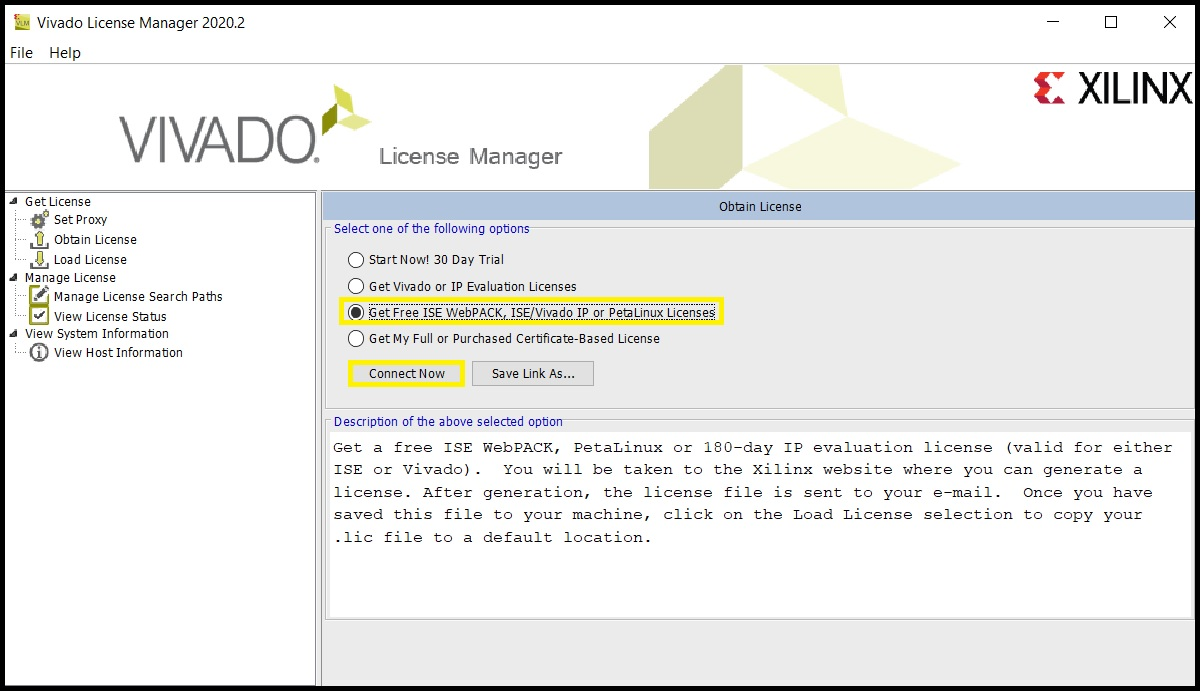
\includegraphics[width=\linewidth]{images/VivadoInstimg023.jpg}
  \end{center}
\end{minipage}

\begin{minipage}{\linewidth}
  Connect with the user account you have created to be able to download the Vivado software.
  If you were not already connected to Xilinx website, this will take you to the main webpage.
  Go back in the licence manager (which is not closed)
  \\
  \begin{center}
    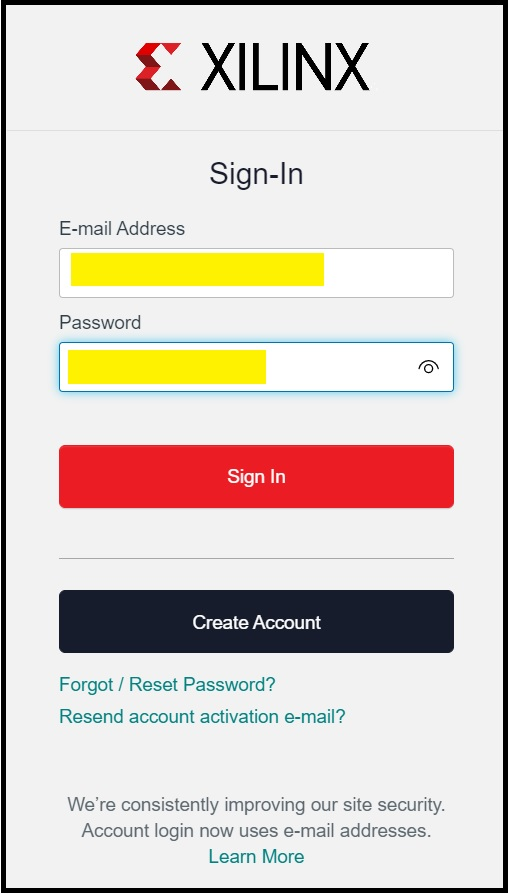
\includegraphics[width=0.3\linewidth]{images/VivadoInstimg024.jpg}
  \end{center}
\end{minipage}

\begin{minipage}{\linewidth}
  Click again on "Connect Now" (ensure "Get Free ISE WebPACK, ISE/Vivado IP or PetaLinux Licenses" is still selected)
  \\
  \begin{center}
    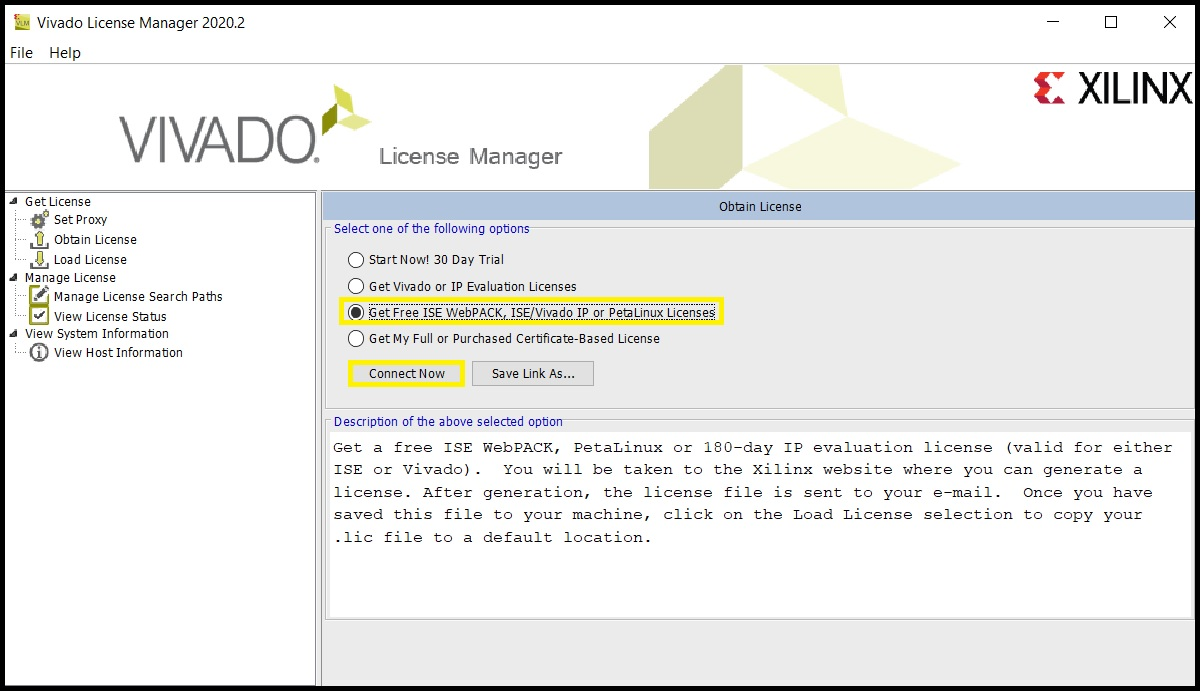
\includegraphics[width=\linewidth]{images/VivadoInstimg023.jpg}
  \end{center}
\end{minipage}

\begin{minipage}{\linewidth}
  You then register your personal information on the Vivado website:
  \\
  \begin{center}
    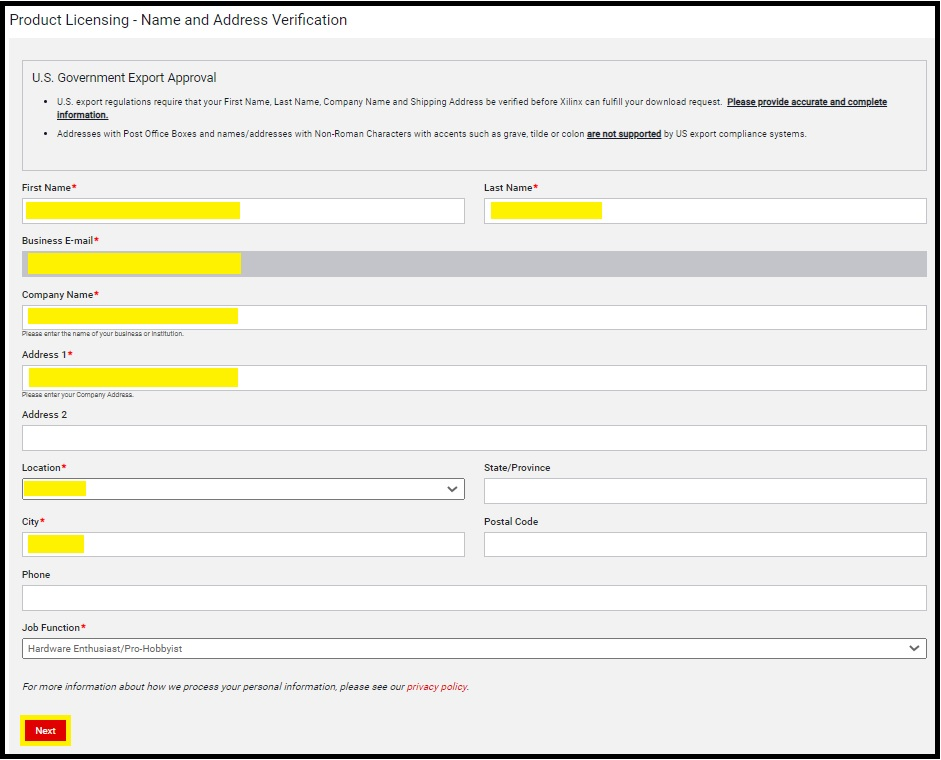
\includegraphics[width=0.7\linewidth]{images/VivadoInstimg025.jpg}
  \end{center}
  Click on "Next".
\end{minipage}


\begin{minipage}{\linewidth}
Select "ISE WebPACK Licence" and "Vivado Design Suite: HL WebPACK 2015 and Earlier License" \\
\\
Then click on "Generate Node-Locked Licence"
\\
\begin{center}
  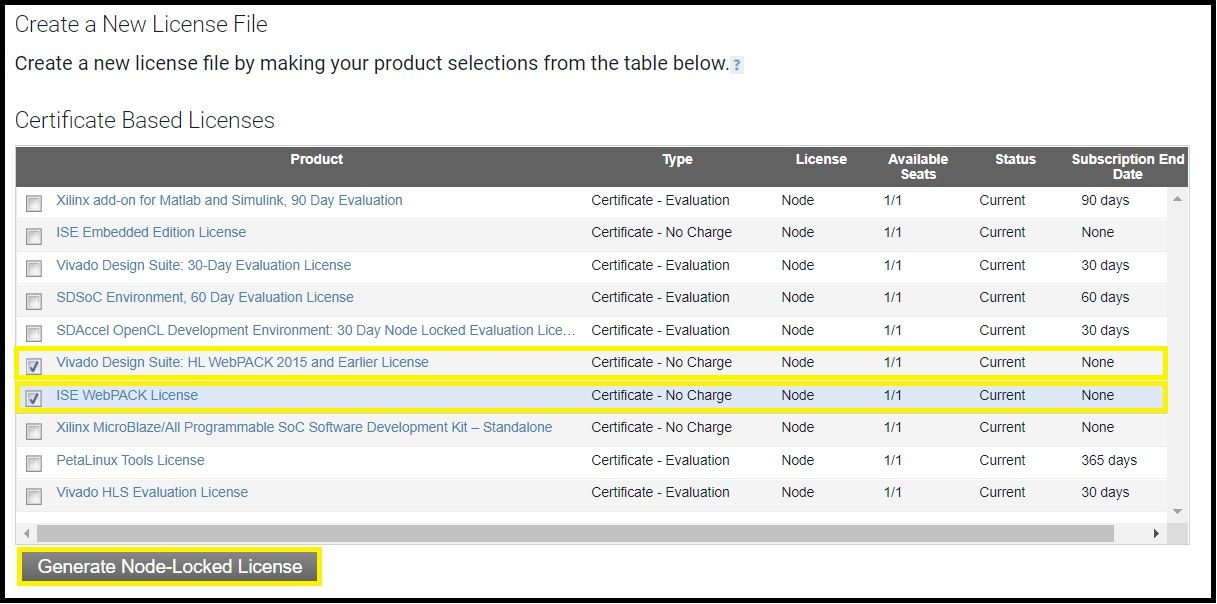
\includegraphics[width=\linewidth]{images/VivadoInstimg026.jpg}
\end{center}
\end{minipage}

\begin{minipage}{\linewidth}
  Click on "Next"
  \\
  \begin{center}
    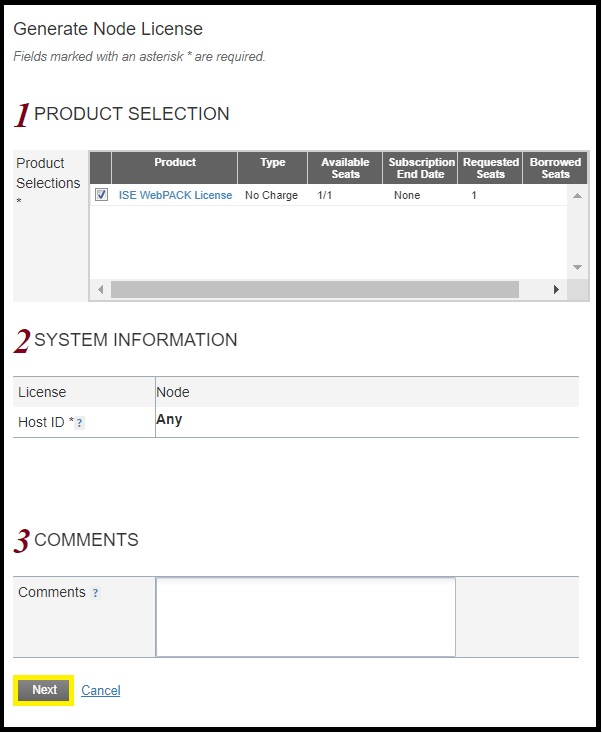
\includegraphics[width=0.5\linewidth]{images/VivadoInstimg027.jpg}
  \end{center}
\end{minipage}

\begin{minipage}{\linewidth}
  Click on "Next"
  \\
  \begin{center}
    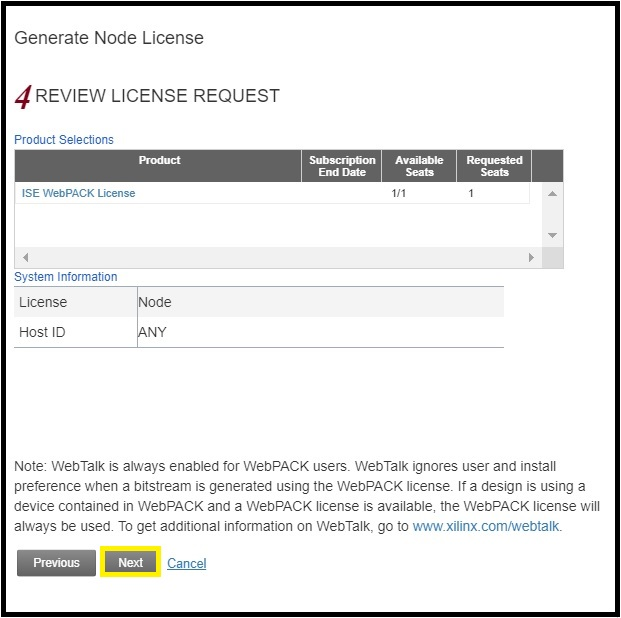
\includegraphics[width=0.5\linewidth]{images/VivadoInstimg028.jpg}
  \end{center}
\end{minipage}


\begin{minipage}{\linewidth}
  Check your email box : You should have received an email from Xilinx, Inc. with a licence file attached and named "Xilinc.lic". \\
  \\
  Retrieve this file on your PC and keep it in safe place.
  \\
  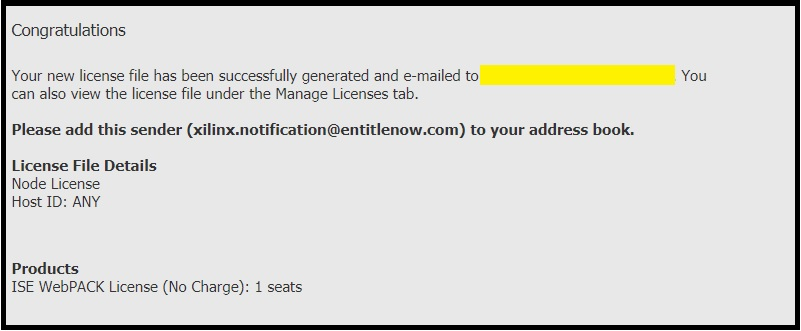
\includegraphics[width=\linewidth]{images/VivadoInstimg029.jpg}
\end{minipage}

\begin{minipage}{\linewidth}
  Go back to the licence manager (which is still running). \\
  \\
  Set "Load License" and click on "Copy License"
  \\
  \begin{center}
    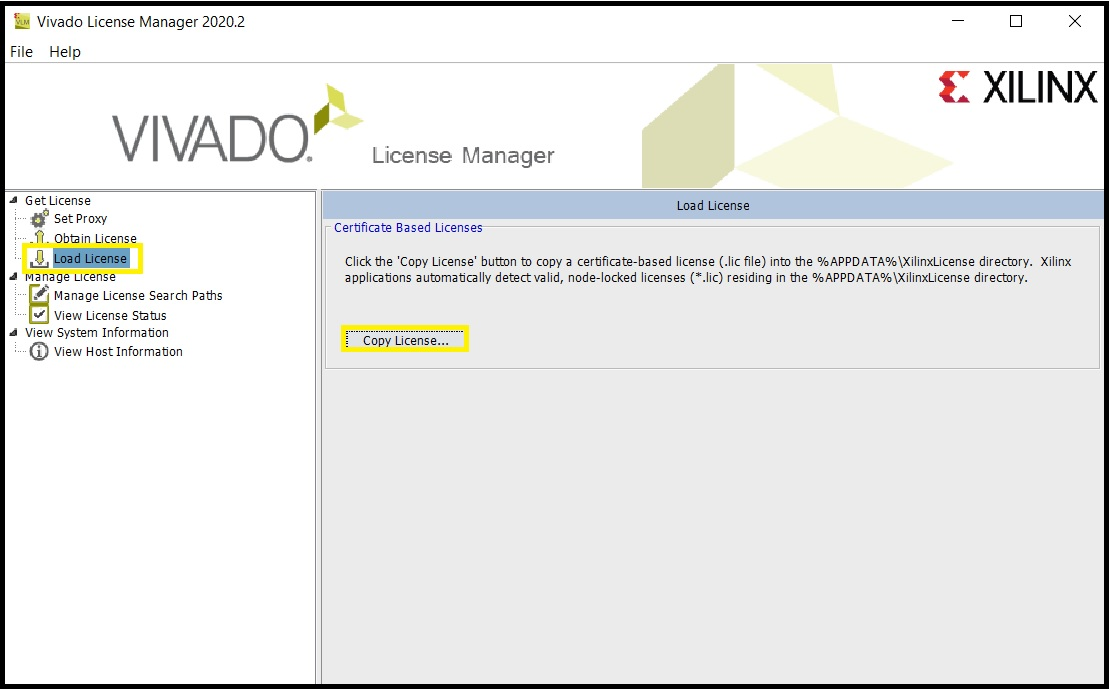
\includegraphics[width=0.8\linewidth]{images/VivadoInstimg030.jpg}
  \end{center}
\end{minipage}

\begin{minipage}{\linewidth}
  Browse to the location where you saved "Xilinc.lic" file, select it and click on "Open".
  \\
  \begin{center}
    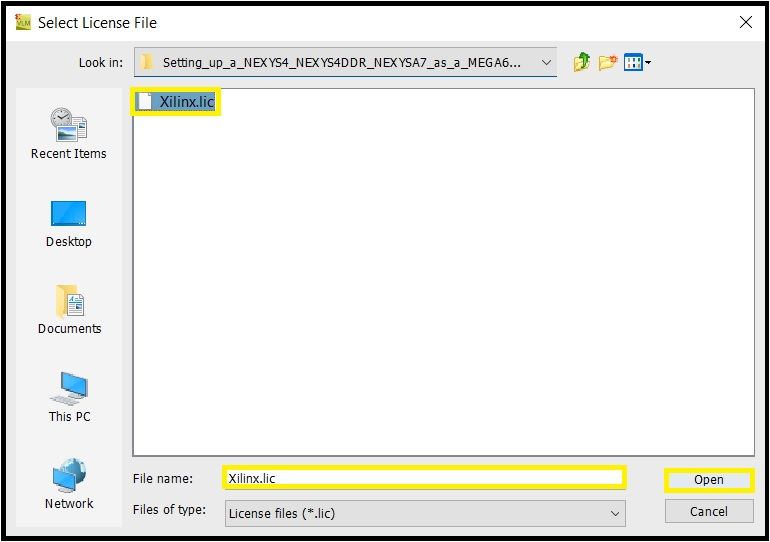
\includegraphics[width=0.7\linewidth]{images/VivadoInstimg031.jpg}
  \end{center}
\end{minipage}

\begin{minipage}{\linewidth}
  Click on "OK" and close the Vivado licence manager.
  \\
  \begin{center}
    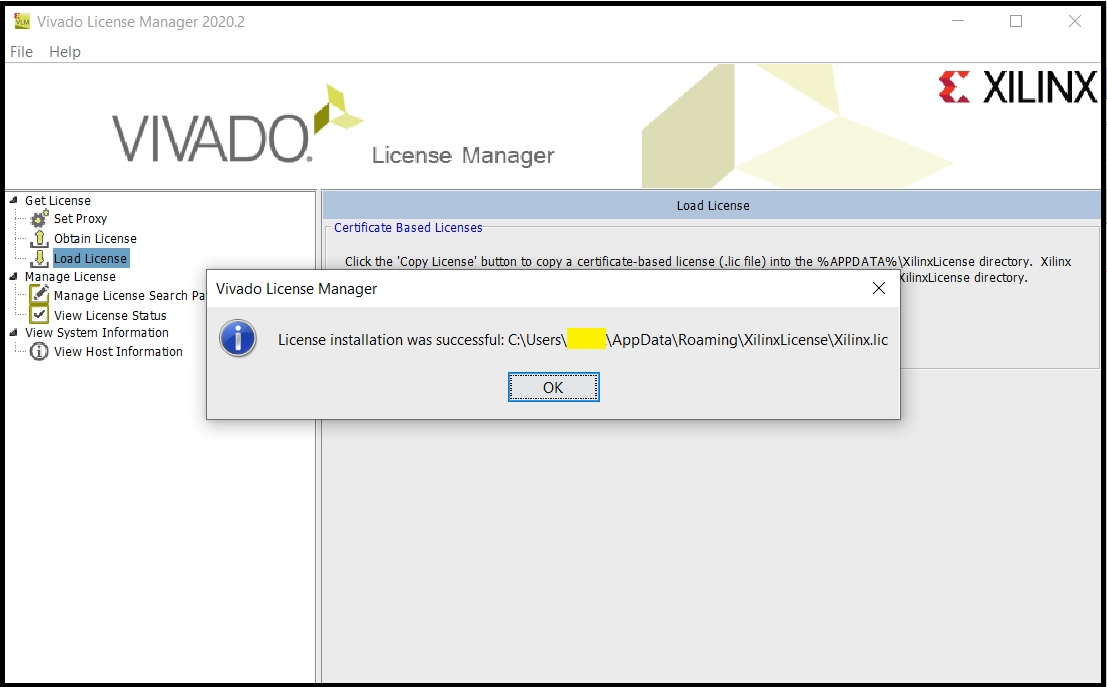
\includegraphics[width=0.7\linewidth]{images/VivadoInstimg032.jpg}
  \end{center}

  Your Vivado software is registered and you can now use it.
\end{minipage}


\section{Flashing the main FPGA of a MEGA65 R2/R3 using Vivado}
\label{sec:mainfpgaflashing}

If you choose to proceed, you will need a TE0790-03 JTAG programming module and a functioning
installation of Xilinx's Vivado software.  This can be done on either Windows or Linux, but
in either case you will need to install any necessary USB drivers. It is
also necessary to have
dip-switches 1 and 3 in the ON position and dip-switches 2 and 4 in the
OFF position on the TE-0790.
With your MEGA65 disconnected from the power, the TE-0790 must be
installed on the JB1 connector which is located between the floppy data cable and the audio jack.
The gold-plated hole of the TE-0790 must line up with the screw
hole below.  The mini-USB cable will then connect on the side towards the 3.5" floppy drive.
The following image shows the correct position: The TE0790 is surrounded by the yellow box,
and the dip-switches by the red box. Dip-switch 1 is the one nearest the floppy data cable.

\includegraphics[width=\linewidth]{images/jtag_detail_02.jpg}

Connect your non-8-bit computer to the FPGA programming device using a
mini-USB cable. Switch the MEGA65 computer ON. Open Vivado, which can
be downloaded from the Internet.

\newpage


\begin{figure}[H]
\centering
  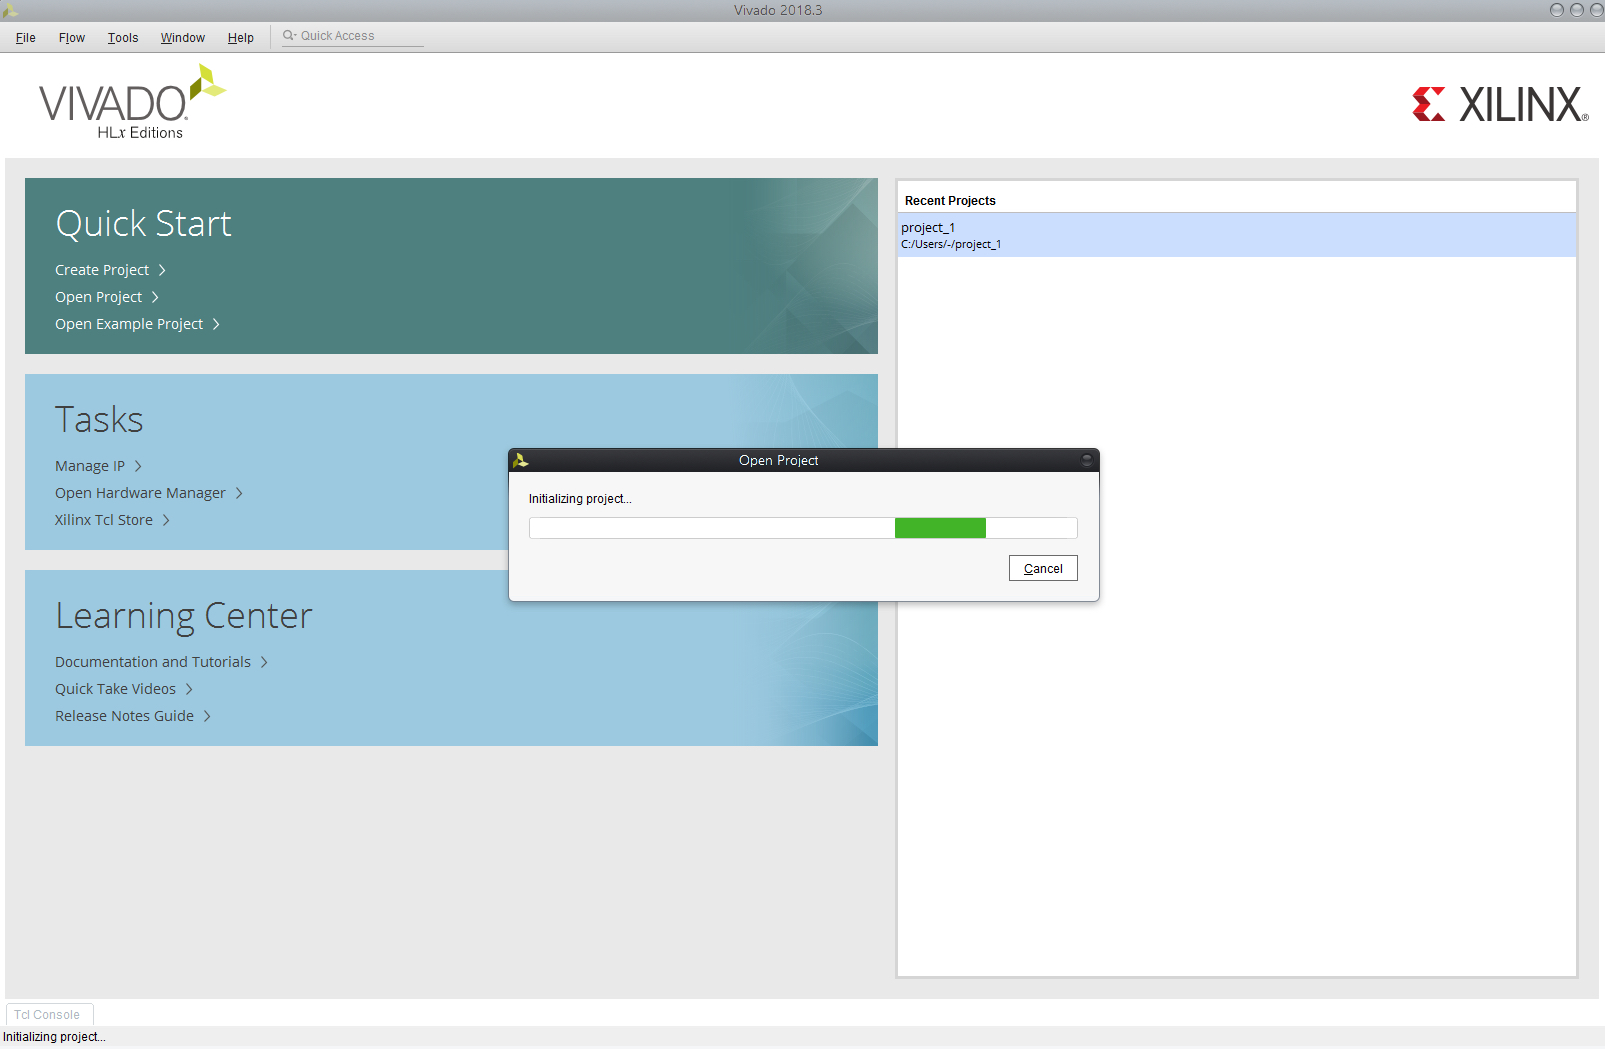
\includegraphics[width=0.8\linewidth]{images/vivado01.png}
  \captionsetup{width=0.8\linewidth}
  \caption{Step 1: To access the Hardware Manager, open a project in
           Vivado or create an empty one, if you do not have any projects yet.}
  \label{fig:vivado01}
%\end{figure}

\vspace{5mm}

%\begin{figure}[H]
\centering
  \includegraphics[width=0.8\linewidth]{images/vivado02.png}
  \captionsetup{width=0.8\linewidth}
  \caption{Step 2: In the left column, select "Open Hardware Manager"
           at the very bottom.}
  \label{fig:vivado02}
\end{figure}


\begin{figure}[H]
  \centering
  \includegraphics[width=0.8\linewidth]{images/vivado03.png}
  \captionsetup{width=0.8\linewidth}
  \caption{Step 3: To connect to FPGA
           under "Hardware Manager", choose "Open Target", then "Auto Connect".}
  \label{fig:vivado03}
%\end{figure}

\vspace{5mm}

%\begin{figure}[H]
  \includegraphics[width=0.8\linewidth]{images/vivado04.png}
  \captionsetup{width=0.8\linewidth}
  \caption{Step 4: Wait a moment, "Connecting to server..."  should
           automatically close without dropping an error to the console.}
  \label{fig:vivado04}
\end{figure}


\begin{figure}[H]
  \centering
  \includegraphics[width=0.8\linewidth]{images/vivado05.png}
  \captionsetup{width=0.8\linewidth}
  \caption{Step 5: Under "Hardware Manager", choose "Add Configuration
           Memory Device", then "xc7a100t\_0".}
  \label{fig:vivado05}
%\end{figure}

\vspace{5mm}

%\begin{figure}[H]
  \includegraphics[width=0.8\linewidth]{images/vivado06.png}
  \captionsetup{width=0.8\linewidth}
  \caption{Step 6: Select Memory Part:
           In the newly opened dialogue, type "S25fl256s"
           (without quotes), then select "s25fl256sxxxxxxx0-spi-x1\_x2\_x4"
           (the upper one) and click "OK".}
  \label{fig:vivado06}
\end{figure}


\begin{figure}[H]
  \centering
  \includegraphics[width=0.85\linewidth]{images/vivado07.png}
  \captionsetup{width=0.85\linewidth}
  \caption{Step 7: Set programming options:
           In the next dialogue, choose your local Configuration file, namely
           a bitstream with file suffix ".mcs". Leave all other parameters
           as they are (see \ref{fig:vivado07}).}
  \label{fig:vivado07}
%\end{figure}

\vspace{3mm}

%\begin{figure}[H]
  \includegraphics[width=0.85\linewidth]{images/vivado08.png}
  \captionsetup{width=0.85\linewidth}
  \caption{Step 8: Patiently wait for the programming to finish.
           This can take several minutes as the Vivado software erases
           and then reprograms the flash memory that is used to
           initialise the FPGA on power-up.}
  \label{fig:vivado08}
\end{figure}


\begin{figure}[H]
  \centering
  \includegraphics[width=0.8\linewidth]{images/vivado09.png}
  \captionsetup{width=0.8\linewidth}
  \caption{Step 9: If your screen looks like \ref{fig:vivado09},
           your new bistream has been successfully flashed into the main FPGA!}
  \label{fig:vivado09}
%\end{figure}

\vspace{5mm}

%\begin{figure}[H]
  \includegraphics[width=0.8\linewidth]{images/vivado09.png}
  \captionsetup{width=0.8\linewidth}
  \caption{Step 10: If you want to reflash the FPGA, you might find the
  "Add Configuration Memory Device" option in step 5 greyed out.
   Instead, select "s25fl256sxxxxxxx0-spi-x1\_x2\_x4"  in the "Hardware"
   window, press right mouse button and select "Program Configuration
   Memory Device" to flash.}
  \label{fig:vivado10}
\end{figure}


\section{Flashing the CPLD in the MEGA65's Keyboard with Lattice Diamond}


If you choose to proceed, you will need a TE0790-03 JTAG programming
module and a functioning installation of Lattice Diamond Programmer software.
This can be done on either Windows or Linux, but in both cases you will
need to install any necessary USB drivers. It is also necessary to have
dip-switches 1 and 3 in the ON position and dip-switches 2 and 4 in the
OFF position on the TE-0790. With your MEGA65 disconnected from the power,
the TE-0790 must be installed on the JB1 connector, which is located
between the floppy data cable and the audio jack.
The gold-plated hole of the TE-0790 must line up with the screw hole below.
The mini-USB cable will then connect on the side towards the 3.5" floppy drive.
The following image shows the correct position: The TE0790 is surrounded
by the yellow box, and the dip-switches by the red box. Dip-switch 1 is
the one nearest the floppy data cable.


\includegraphics[width=\linewidth]{images/jtag_detail_05.jpg}


On the PCB R2 MEGA65 mainboard, dip switch 1 (the one nearest to the user
sitting in front of the machine) must be in the ON position. The other
switches must be OFF. The keyboard will go into ``ambulance mode''
(blue flashing lights) when set correctly.

Connect your non-8-bit computer to the FPGA programming device using a
mini-USB cable. Switch the MEGA65 computer ON. Open the Diamond Programmer
which can be downloaded from the Internet.

\begin{figure}[H]
  \centering
  \includegraphics{images/diamond01.png}
  \captionsetup{width=0.8\linewidth}
  \caption{Step 1: Open DIAMOND PROGRAMMER:
           Select "Create a new project from a JTAG scan". If entry
           under "Cable:" is empty, click "Detect Cable".}
  \label{fig:diamond01}
%\end{figure}

\vspace{5mm}

%\begin{figure}[H]
  \includegraphics[width=0.8\linewidth]{images/diamond02.png}
  \captionsetup{width=0.8\linewidth}
  \caption{Step 2: Create a new project:
           If dialog "Programmer: Multiple Cables Detected" appears,
           select the first entry ("Location 0000") and click "OK".}
  \label{fig:diamond02}
\end{figure}


\begin{figure}[H]
  \centering
  \includegraphics[width=0.8\linewidth]{images/diamond03.png}
  \captionsetup{width=0.8\linewidth}
  \caption{Step 3: Select cable:
           You have now created a new project which should display
           "MachXO2" under "Device Family" and "LCMXO2-1200HC" under "Device"}
  \label{fig:diamond03}
%\end{figure}

\vspace{5mm}

%\begin{figure}[H]
  \includegraphics[width=0.8\linewidth]{images/diamond04.png}
  \captionsetup{width=0.8\linewidth}
  \caption{Step 4: New Diamond Programmer project:
           Choose "File" then "Open File" to load the Diamond Pprogrammer
           project with the MEGA65 keyboard firmware update.}
  \label{fig:diamond04}
\end{figure}


\begin{figure}[H]
  \centering
  \includegraphics[width=0.8\linewidth]{images/diamond05.png}
  \captionsetup{width=0.8\linewidth}
  \caption{Step 5: Open project:
           Navigate into the folder with the extracted MEGA65 keyboard
           firmware files you have received and select the file ending with ".xcf".}
  \label{fig:diamond05}
%\end{figure}

\vspace{5mm}

%\begin{figure}[H]
  \includegraphics[width=0.8\linewidth]{images/diamond06.png}
  \captionsetup{width=0.8\linewidth}
  \caption{Step 6: Select project file:
           Click the three dots under "File Name" to set the correct
           path and find the file ending with ".jed".}
  \label{fig:diamond06}
\end{figure}


\begin{figure}[H]
  \centering
  \includegraphics[width=0.8\linewidth]{images/diamond07.png}
  \captionsetup{width=0.8\linewidth}
  \caption{Step 7: Choose correct path of .jed file:
           Select the file ending with ".jed" and click "OK".}
  \label{fig:diamond07}
%\end{figure}

\vspace{5mm}

%\begin{figure}[H]
  \includegraphics[width=0.8\linewidth]{images/diamond08.png}
  \captionsetup{width=0.8\linewidth}
  \caption{Step 8: Select .jed file:
           Click on the icon with the green arrow facing down "PROGRAM",
           which looks similar to the Diamond Programmer program icon.}
  \label{fig:diamond08}
\end{figure}


\begin{figure}[H]
  \centering
  \includegraphics[width=0.8\linewidth]{images/diamond09.png}
  \captionsetup{width=0.8\linewidth}
  \caption{Step 9: Select cable:
           After a moment the Output window should display
           "INFO - Operation: successful." and the "Status" cell should
           go green (does not always happen).}
  \label{fig:diamond09}
%\end{figure}

\vspace{5mm}

%\begin{figure}[H]
  \includegraphics[width=0.8\linewidth]{images/diamond10.png}
  \captionsetup{width=0.8\linewidth}
  \caption{Step 10: Operation successful:
           You have now successfully flashed the MEGA65 keyboard.
           If you wish you can now save the project for later use.}
  \label{fig:diamond10}
\end{figure}


\section{Flashing the MAX10 FPGA on the MEGA65's Mainboard with INTEL QUARTUS}

If you choose to proceed, you will need a TEI0004 - Arrow USB Programmer2 module with TEI0004 driver installed
and a functioning installation of Quartus Prime Programmer Lite Edition.  This can be done on either Windows
or Linux, but in both cases you will need to install any necessary USB drivers.
With your MEGA65 disconnected from the power, the TEI0004 must be installed on the J17 connector,
which is located between the floppy data cable and the ARTIX 7 FPGA on the Mainboard.
The micro-USB port of the TEI0004 must face in the opposite direction of the HDMI and LAN sockets, towards
the trap door.
The following image shows the correct position.

On the PCB R2 MEGA65 mainboard, all dip switches must be in the OFF position. The main FPGA of the MEGA65 R2 must not contain
a valid bitstream. See section \nameref{sec:mainfpgaflashing} on how to erase the bitstream
from the main FPGA.

\includegraphics[width=\linewidth]{images/jtag_detail_05.jpg}

Connect your non-8-bit computer to the FPGA programming device using a micro-USB cable.
Open Quartus Prime Programmer Lite Edition, which can be downloaded from the Internet.

\begin{figure}[H]
  \centering
  \includegraphics{images/max10_01.png}
  \captionsetup{width=0.8\linewidth}
  \caption{Step 1: Open Quartus Prime Programmer Lite Edition:
           Click the "Hardware Setup" button in the top left corner of
           the Quartus Prime Programmer window.}
  \label{fig:max10_01}
%\end{figure}

\vspace{5mm}

%\begin{figure}[H]
  \includegraphics[width=0.8\linewidth]{images/max10_02.png}
  \captionsetup{width=0.8\linewidth}
  \caption{Step 2: Enter Hardware Setup:
           In the newly appeared window under "Currently selected
           hardware" choose "Arrow-USB-Blaster".
           If "Arrow-USB-Blaster" does not appear, verify cable and
           drivers being correctly installed.}
  \label{fig:max10_02}
\end{figure}


\begin{figure}[H]
  \centering
  \includegraphics[width=0.8\linewidth]{images/max10_03.png}
  \captionsetup{width=0.8\linewidth}
  \caption{Step 3: Select Arrow USB-Blaster:
           Click the "Add File" button from the left row and choose the
           latest ".pof" file. Then click "Open".}
  \label{fig:max10_03}
\end{figure}


\begin{figure}[H]
  \centering
  \includegraphics[width=0.7\linewidth]{images/max10_04.png}
  \captionsetup{width=0.7\linewidth}
  \caption{Step 4: Select Programming File:
           Tick at least the three boxes under "Program/Configure".
           Also enabling all boxes under "Verify" and "Blank-Check"
           will make the process more reliable.}
  \label{fig:max10_04}
%\end{figure}

\vspace{5mm}

%\begin{figure}[H]
  \includegraphics[width=0.7\linewidth]{images/max10_05.png}
  \captionsetup{width=0.7\linewidth}
  \caption{Step 5: Select Program/Configure Options}
  \label{fig:max10_05}
\end{figure}

While keeping the Reset-Button pressed, switch the MEGA65 computer ON.
The keyboard will go into ``ambulance mode'' (blue flashing lights).
If it does not, the main FPGA is not empty - restart the whole process.

Now click on "Start" in the left row of buttons. The progress bar in
the top right corner should quickly go to 100 percent and turn green.
You have now successfully updated your MAX10 FPGA.

If you receive an error message instead, make sure the main FPGA
bitstream has been erased and that you did not release the reset-button on
the MEGA65 beforehand. Switch off the MEGA65 and restart this step.

\begin{figure}[H]
  \centering
  \includegraphics[width=0.8\linewidth]{images/max10_06.png}
  \captionsetup{width=0.8\linewidth}
  \caption{Step 6: Programming successful}
  \label{fig:max10_06}
\end{figure}


  \lstset{
    basicstyle=\small\ttfamily,
    columns=flexible,
    breaklines=true
}

\chapter{Trouble shooting}

\section{Hardware}
    \subsection{No lights when powering on}
    If there are occasions when your MEGA65 display any lights when powering on, they relate to having certain Digital Video devices plugged in while the MEGA65 is off, that don't provide enough power for the keyboard's CPLD to be properly powered on, but enough to stop it properly resetting when the MEGA65 powers on. Removing the Digital Video cable and switching the machine off and on again fixes the issue.

\section{Vivado}
    \subsection{RAM requirements}
    \begin{tcolorbox}[colback=black,coltext=white]
    \begin{lstlisting}
INFO: [Synth 8-256] done synthesizing module 'ram32x1024' [/home/....]
INFO: [Synth 8-256] synthesizing module 'charrom' [/home/....]
    /opt/Xilinx/Vivado/2019.2/bin/loader: line 280: 2317 killed
    WARNING: [Vivado 12-8222] Failed run(s) : 'synth\_1'
        ERROR: Application Exception: failed to launch run 'impl\_1' due to failures in the following run(s):
        synth\_1
        These failed run(s) need to be reset prior to launching 'impl\_1' again.
    \end{lstlisting}
    \end{tcolorbox}
This error is due to Vivado crashing because the machine doesn't have enough RAM for Vivado to run.
Vivado requires at least 4GB to synthesise the MEGA65 target, but 8GB is better.

\section{mega65\_ftp}
    \subsection{Missing Library}
    \begin{tcolorbox}[colback=black,coltext=white]
\begin{lstlisting}
/usr/bin/ld: cannot find -lncurses
collect2: error: ld returned 1 exit status
Makefile:474: recipe for target 'bin/mega65_ftp' failed
make: *** [bin/mega65_ftp] Error 1\end{lstlisting}
    \end{tcolorbox}
This error occurs when the ncurses library is missing from the computer when building the mega65\_ftp program.
To rectify this issue you will need to ensure that you install this dependency.

    \begin{tcolorbox}[colback=black,coltext=white]
\begin{lstlisting}
sudo apt-get install libncurses5-dev libncursesw5-dev\end{lstlisting}
    \end{tcolorbox}


  \chapter{Schematics}
\section{MEGA65 R3 Schematics}
\includepdf[landscape,pages=-,turn=false]{assets/TE0765-03.PDF}
\section{MEGA65 R2 Schematics}
\includepdf[landscape,pages=-,turn=false]{assets/TE0765-02.PDF}
\section{Nexys Widget Board Schematics}
\label{sec:nexyswidgetschematics}
\includepdf[landscape,pages=-,turn=false]{assets/nexys-widget-board-sch.pdf}
\includepdf[portrait,pages=-,turn=false]{assets/nexys-widget-board-pcb.pdf}

  \chapter{Supporters \& Donors}


The MEGA65 would not have been possible to create without the generous support
of many organisations and individuals.

We are still compiling these lists, so apologies if we haven't included you yet.  If you
know anyone we have left out, please let us know, so that we can recognise the contribution
of everyone who has made the MEGA65 possible, and into the great retro-computing project
that it has become.

\section{Organisations}

{\bf The MEGA Museum of Electronic Games \& Art e.V. Germany} \\
\megakey{Everything}

{\bf Trenz Electronik, Germany} \\
\megakey{Motherboard}

{\bf Hintsteiner, Austria} \\
\megakey{Case}

{\bf GMK, Germany} \\
\megakey{Keyboard}

\section{Contributors}

\begin{tabular}{p{6cm}p{6cm}}

{\large\bf Andreas Liebeskind}     & {\large\bf Dr. Canan Hastik} \\
 \textit{(libi in paradize)}       & \textit{(indica)} \\
CFO MEGA eV                        & Chairwoman MEGA eV \\
& \\
{\large\bf Gurce Isikyildiz}       & {\large\bf Simon Jameson} \\
 \textit{(Gurce)}                  &  \textit{(Shallan)} \\
Tools and enhancements             & Platform Enhancements \\
& \\
{\large\bf Russell Peake}          & {\large\bf Stephan Kleinert} \\
  \textit{(rdpeake)}               & \textit{(ubik)}        \\
Bug Herding                        & Destroyer of BASIC 10     \\
& \\
{\large\bf Alexander Nik Petra}    & {\large\bf Wayne Johnson} \\
 \textit{(n0d)}                    &  \textit{(sausage)} \\
Early Case Design                  & Manual Additions \\
& \\
{\large\bf Ralph Egas}             & {\large\bf Lukas Kleiss} \\
 \textit{(0-limits)}               & \textit{(LAK132)} \\
Business Advisor                   & MegaWAT Presentation Software \\
& \\
{\large\bf Lucas Moss}             & {\large\bf Maurice van Gils }  \\
                                   & \textit{(Maurice)}  \\
MEGAphone PCB Design               & BASIC 65 example programs \\
& \\
{\large\bf Daren Klamer}           & \\
 \textit{(Impakt)}                 & \\
Manual proof-reading               & \\
\end{tabular}

\newpage
\section{Supporters}

\begin{small}
% page 1
\setlength{\tabcolsep}{1mm}
\begin{tabular}{p{4cm}p{4cm}p{4cm}}
@11110110100 & Arne Neumann & Christian Gräfe \\
3c74ce64 & Arne Richard Tyarks & Christian Heffner \\
8-Bit Classics & Axel Klahr & Christian Kersting \\
Aaron Smith & Balaz Ondrej & Christian Schiller \\
Achim Mrotzek & Barry Thompson & Christian Streck \\
Adolf Nefischer & Bartol Filipovic & Christian Weyer \\
Adrian Esdaile & Benjamin Maas & Christian Wyk \\
Adrien Guichard & Bernard Alaiz & Christoph Haug \\
Ahmed Kablaoui & Bernhard Zorn & Christoph Huck \\
Alan Bastian Witkowski & Bieno Marti-Braitmaier & Christoph Pross \\
Alan Field & Bigby & Christopher Christopher \\
Alastair Paulin-Campbell & Bill LaGrue & Christopher Kalk \\
Alberto Mercuri & Bjoerg Stojalowski & Christopher Kohlert \\
Alexander Haering & Björn Johannesson & Christopher Nelson \\
Alexander Kaufmann & Bjørn Melbøe & Christopher Taylor \\
Alexander Niedermeier & Bo Goeran Kvamme & Christopher Whillock \\
Alexander Soppart & Boerge Noest & Claudio Piccinini \\
Alfonso Ardire & Bolko Beutner & Claus Skrepek \\
Amiga On The Lake & Brett Hallen & Collen Blijenberg \\
André Kudra & Brian Gajewski & Constantine Lignos \\
André Simeit & Brian Green & Crnjaninja \\
André Wösten & Brian Juul Nielsen & Daniel Auger \\
Andrea Farolfi & Brian Reiter & Daniel Julien \\
Andrea Minutello & Bryan Pope & Daniel Lobitz \\
Andreas Behr & Burkhard Franke & Daniel O'Connor \\
Andreas Freier & Byron Goodman & Daniel Teicher \\
Andreas Grabski & Cameron Roberton (KONG) & Daniel Tootill \\
Andreas Millinger & Carl Angervall & Daniel Wedin \\
Andreas Nopper & Carl Danowski & Daniele Benetti \\
Andreas Ochs & Carl Stock & Daniele Gaetano Capursi \\
Andreas Wendel Manufaktur & Carl Wall & Dariusz Szczesniak \\
Andreas Zschunke & Carlo Pastore & Darrell Westbury \\
Andrew Bingham & Carlos Silva & David Asenjo Raposo \\
Andrew Dixon & Carsten Sørensen & David Dillard \\
Andrew Mondt & Cenk Miroglu Miroglu & David Gorgon \\
Andrzej Hłuchyj & Chang sik Park & David Norwood \\
Andrzej Sawiniec & Charles A. Hutchins Jr. & David Raulo \\
Andrzej Śliwa & Chris Guthrey & David Ross \\
Anthony W. Leal & Chris Hooper & de voughn accooe \\
Arkadiusz Bronowicki & Chris Stringer & Dean Scully \\
Arkadiusz Kwasny & Christian Boettcher & Dennis Jeschke \\
Arnaud Léandre & Christian Eick & Dennis Schaffers \\
Arne Drews & Christian Gleinser & Dennis Schierholz \\
\end{tabular}
% page 2
\newpage
\setlength{\tabcolsep}{1mm}
\begin{tabular}{p{4cm}p{4cm}p{4cm}}
Dennis Schneck & Frank Haaland & Hendrik Fensch \\
denti & Frank Hempel & Henning Harperath \\
Dick van Ginkel & Frank Koschel & Henri Parfait \\
Diego Barzon & Frank Linhares & Henrik Kühn \\
Dierk Schneider & Frank Sleeuwaert & Holger Burmester \\
Dietmar Krueger & Frank Wolf & Holger Sturk \\
Dietmar Schinnerl & FranticFreddie & Howard Knibbs \\
Dirk Becker & Fredrik Ramsberg & Hubert de Hollain \\
Dirk Wouters & Fridun Nazaradeh & Huberto Kusters \\
Domingo Fivoli & Friedel Kropp & Hugo Maria Gerardus v.d. Aa \\
DonChaos & Garrick West & Humberto Castaneda \\
Donn Lasher & Gary Lake-Schaal & Ian Cross \\
Douglas Johnson & Gary Pearson & IDE64 Staff \\
Dr. Leopold Winter & Gavin Jones & Igor Ianov \\
Dusan Sobotka & Geir Sigmund Straume & Immo Beutler \\
Earl Woodman & Gerd Mitlaender & Ingo Katte \\
Ed Reilly & Giampietro Albiero & Ingo Keck \\
Edoardo Auteri & Giancarlo Valente & Insanely Interested Publishing \\
Eduardo Gallardo & Gianluca Girelli & IT-Dienstleistungen Obsieger \\
Eduardo Luis Arana & Giovanni Medina & Ivan Elwood \\
Eirik Juliussen Olsen & Glen Fraser & Jaap HUIJSMAN \\
Emilio Monelli & Glen R Perye III & Jace Courville \\
EP Technical Services & Glenn Main & Jack Wattenhofer \\
Epic Sound & Gordon Rimac & Jakob Schönpflug \\
Erasmus Kuhlmann & GRANT BYERS & Jakub Tyszko \\
ergoGnomik & Grant Louth & James Hart \\
Eric Hilaire & Gregor Bubek & James Marshburn \\
Eric Hildebrandt & Gregor Gramlich & James McClanahan \\
Eric Hill & Guido Ling & James Sutcliffe \\
Eric Jutrzenka & Guido von Gösseln & Jan Bitruff \\
Erwin Reichel & Guillaume Serge & Jan Hildebrandt \\
Espen Skog & Gunnar Hemmerling & Jan Iemhoff \\
Evangelos Mpouras & Günter Hummel & Jan Kösters \\
Ewan Curtis & Guy Simmons & Jan Peter Borsje \\
Fabio Zanicotti & Guybrush Threepwood & Jan Schulze \\
Fabrizio Di Dio & Hakan Blomqvist & Jan Stoltenberg-Lerche \\
Fabrizio Lodi & Hans Pronk & Janne Tompuri \\
FARA Gießen GmbH & Hans-Jörg Nett & Jannis Schulte \\
FeralChild & Hans-Martin Zedlitz & Jari Loukasmäki \\
First Choice Auto's & Harald Dosch & Jason Smith \\
Florian Rienhardt & Harri Salokorpi & Javier Gonzalez Gonzalez \\
Forum64. de & Harry Culpan & Jean-Paul Lauque \\
Francesco Baldassarri & Heath Gallimore & Jeffrey van der Schilden \\
Frank Fechner & Heinz Roesner & Jens Schneider \\
Frank Glaush & Heinz Stampfli & Jens-Uwe Wessling \\
Frank Gulasch & Helge Förster & Jesse DiSimone \\
\end{tabular}
% page 3
\newpage
\setlength{\tabcolsep}{1mm}
\begin{tabular}{p{4cm}p{4cm}p{4cm}}
Jett Adams & Kevin Thomasson & Marco van de Water \\
Johan Arneklev & Kim Jorgensen & Marcus Gerards \\
Johan Berntsson & Kim Rene Jensen & Marcus Herbert \\
Johan Svensson & Kimmo Hamalainen & Marcus Linkert \\
Johannes Fitz & Konrad Buryło & Marek Pernicky \\
John Cook & Kosmas Einbrodt & Mario Esposito \\
John Deane & Kurt Klemm & Mario Fetka \\
John Dupuis & Lachlan Glaskin & Mario Teschke \\
John Nagi & Large bits collider & Mariusz Tymków \\
John Rorland & Lars Becker & Mark Adams \\
John Sargeant & Lars Edelmann & Mark Anderson \\
John Traeholt & Lars Slivsgaard & Mark Green \\
Jon Sandelin & Lasse Lambrecht & Mark Hucker \\
Jonas Bernemann & Lau Olivier & Mark Leitiger \\
Jonathan Prosise & Lee Chatt & Mark Spezzano \\
Joost Honig & Loan Leray & Mark Watkin \\
Jordi Pakey-Rodriguez & Lorenzo Quadri & Marko Rizvic \\
Jöre Weber & Lorenzo Travagli & Markus Bieler \\
Jörg Jungermann & Lorin Millsap & Markus Bonet \\
Jörg Schaeffer & Lothar James Foss & Markus Dauberschmidt \\
Jörg Weese & Lothar Serra Mari & Markus Fehr \\
Josef Hesse & Luca Papinutti & Markus Fuchs \\
Josef Soucek & Ludek Smetana & Markus Guenther-Hirn \\
Josef Stohwasser & Lukas Burger & Markus Liukka \\
Joseph Clifford & Lutz-Peter Buchholz & Markus Merz \\
Joseph Gerth & Luuk Spaetgens & Markus Roesgen \\
Jovan Crnjanin & Mad Web Skills & Markus Uttenweiler \\
Juan Pablo Schisano & MaDCz & Martin Bauhuber \\
Juan S. Cardona Iguina & Magnus Wiklander & Martin Benke \\
JudgeBeeb & Maik Diekmann & Martin Gendera \\
Juliussen Olsen & Malte Mundt & Martin Groß \\
Juna Luis Fernandez Garcia & Manfred Wittemann & Martin Gutenbrunner \\
Jürgen Endras & Manuel Beckmann & Martin Johansen \\
Jürgen Herm Stapelberg & Manzano Mérida & Martin Marbach \\
Jyrki Laurila & Marc "3D-vice" Schmitt & Martin Sonnleitner \\
Kai Pernau & Marc Bartel & Martin Steffen \\
Kalle Pöyhönen & Marc Jensen & Marvin Hardy \\
Karl Lamford & Marc Schmidt & Massimo Villani \\
Karl-Heinz Blum & Marc Theunissen & Mathias Dellacherie \\
Karsten Engstler & Marc Tutor & Mathieu Chouinard \\
Karsten Westebbe & Marc Wink & Matthew Adams \\
katarakt & Marcel Buchtmann & Matthew Browne \\
Keith McComb & Marcel Kante & Matthew Carnevale \\
Kenneth Dyke & Marco Beckers & Matthew Palmer \\
Kenneth Joensson & Marco Cappellari & Matthew Santos \\
Kevin Edwards & Marco Rivela & Matthias Barthel \\
\end{tabular}
% page 4
\newpage
\setlength{\tabcolsep}{1mm}
\begin{tabular}{p{4cm}p{4cm}p{4cm}}
Matthias Dolenc & Mikael Lund & Paul Kuhnast (mindrail) \\
Matthias Fischer & Mike Betz & Paul Massay \\
Matthias Frey & Mike Kastrantas & Paul Westlake \\
Matthias Grandis & Mike Pikowski & Paul Wögerer \\
Matthias Guth & Mikko Hämäläinen & Pauline Brasch \\
Matthias Lampe & Mikko Suontausta & Paulo Apolonia \\
Matthias Meier & Mirko Roller & Pete Collin \\
Matthias Mueller & Miroslav Karkus & Pete of Retrohax.net \\
Matthias Nofer & Morgan Antonsson & Peter Eliades \\
Matthias Schonder & Moritz & Peter Gries \\
Maurice Al-Khaliedy & Morten Nielsen & Peter Habura \\
Max Ihlenfeldt & MUBIQUO APPS,SL & Peter Herklotz \\
Meeso Kim & Myles Cameron-Smith & Peter Huyoff \\
Michael Dailly & Neil Moore & Peter Knörzer \\
Michael Dötsch & Nelson & Peter Leswell \\
Michael Dreßel & neoman & Peter Weile \\
Michael Fichtner & Nicholas Melnick & Petri Alvinen \\
Michael Fong & Nikolaj Brinch Jørgensen & Philip Marien \\
Michael Geoffrey Stone & Nils Andreas & Philip Timmermann \\
Michael Gertner & Nils Eilers & Philipp Rudin \\
Michael Grün & Nils Hammerich & Pierre Kressmann \\
Michael Habel & Nils77 & Pieter Labie \\
Michael Härtig & Norah Smith & Piotr Kmiecik \\
Michael Haynes & Norman King & Power-on.at \\
Michael J Burkett & Normen Zoch & Przemysław Safonow \\
Michael Jensen & Olaf Grunert & Que Labs \\
Michael Jurisch & Ole Eitels & R Welbourn \\
Michael Kappelgaard & Oliver Boerner & R-Flux \\
Michael Kleinschmidt & Oliver Brüggmann & Rafał Michno \\
Michael Lorenz & Oliver Graf & Rainer Kappler \\
Michael Mayerhofer & Oliver Smith & Rainer Kopp \\
Michael Nurney & Olivier Bori & Rainer Weninger \\
Michael Rasmussen & ONEPSI LLC & Ralf Griewel \\
Michael Richmond & oRdYNe & Ralf Pöscha \\
Michael Sachse & Osaühing Trioflex & Ralf Reinhardt \\
Michael Sarbak & OSHA-PROS USA & Ralf Schenden \\
Michael Schneider & Padawer & Ralf Smolarek \\
Michael Scholz & Patrick Becher & Ralf Zenker \\
Michael Timm & Patrick Bürckstümmer & Ralph Bauer \\
Michael Traynor & Patrick de Zoete & Ralph Wernecke \\
Michael Whipp & Patrick Toal & Rédl Károly \\
Michal Ursiny & Patrick Vogt & Reiner Lanowski \\
Michele Chiti & Paul Alexander Warren & Remi Veilleux \\
Michele Perini & Paul Gerhardt (KONG) & Riccardo Bianchi \\
Michele Porcu & Paul Jackson & Richard Englert \\
Miguel Angel Rodriguez Jodar & Paul Johnson & Richard Good \\
\end{tabular}
% page 5
\newpage
\setlength{\tabcolsep}{1mm}
\begin{tabular}{p{4cm}p{4cm}p{4cm}}
Richard Menedetter & Simon Lawrence & Thomas Schilling \\
Richard Sopuch & Simon Wolf & Thomas Tahsin-Bey \\
Rick Reynolds & spreen.digital & Thomas Walter \\
Rico Gruninger & Stefan Haberl & Thomas Wirtzmann \\
Rob Dean & Stefan Kramperth & Thorsten Knoll \\
Robert Bernardo & Stefan Richter & Thorsten Nolte \\
Robert Eaglestone & Stefan Schultze & Tim Krome \\
Robert Grasböck & Stefan Sonnek & Tim Waite \\
Robert Miles & Stefan Theil & Timo Weirich \\
Robert Schwan & Stefan Vrampe & Timothy Blanks \\
Robert Shively & Stefano Canali & Timothy Henson \\
Robert Tangmar & Stefano Mozzi & Timothy Prater \\
Robert Trangmar & Steffen Reiersen & Tobias Butter \\
Rodney Xerri & Stephan Bielmann & Tobias Heim \\
Roger Olsen & Stephen Jones & Tobias Köck \\
Roger Pugh & Stephen Kew & Tobias Lüthi \\
Roland Attila Kett & Steve Gray & Tommi Vasarainen \\
Roland Evers & Steve Kurlin & Toni Ammer \\
Roland Schatz & Steve Lemieux & Tore Olsen \\
Rolf Hass & Steven Combs & Torleif Strand \\
Ronald Cooper & Stewart Dunn & Torsten Schröder \\
Ronald Hunn & Stuart Marsh & Tuan Nguyen \\
Ronny Hamida & Sven Neumann & Uffe Jakobsen \\
Ronny Preiß & Sven Stache & Ulrich Hintermeier \\
Roy van Zundert & Sven Sternberger & Ulrich Nieland \\
Rüdiger Wohlfromm & Sven Wiegand & Ulrik Kruse \\
Ruediger Schlenter & Szabolcs Bence & Ursula Förstle \\
Rutger WIllemsen & Tantrumedia Limited & Uwe Anfang \\
Sampo Peltonen & Techvana Operations Ltd. & Uwe Boschanski \\
Sarmad Gilani & Teddy Turmeaux & Vedran Vrbanc \\
SAS74 & Teemu Korvenpää & Verm Project \\
Sascha Hesse & The Games Foundation & Wayne Rittimann \\
Scott Halman & Thierry Supplisson & Wayne Sander \\
Scott Hollier & Thieu-Duy Thai & Wayne Steele \\
Scott Robison & Thomas Bierschenk & Who Knows \\
Sebastian Baranski & Thomas Edmister & Winfried Falkenhahn \\
Sebastian Bölling & Thomas Frauenknecht & Wolfgang Becker \\
Sebastian Felzmann & Thomas Gitzen & Wolfgang Stabla \\
Sebastian Lipp & Thomas Gruber & Worblehat \\
Sebastian Rakel & Thomas Haidler & www.patop69.net \\
Şemseddin Moldibi & Thomas Jager & Yan B \\
Seth Morabito & Thomas Karlsen & Zoltan Markus \\
Shawn McKee & Thomas Laskowski & Zsolt Zsila \\
Siegfried Hartmann & Thomas Marschall & Zytex Online Store \\
Sigurbjorn Larusson & Thomas Niemann &  \\
Sigurdur Finnsson & Thomas Scheelen &  \\
\end{tabular}
\end{small}
\ifdefined\printmanual
\else
\setstretch{1}
\fi



\nocite{*}
\bibliographystyle{IEEEtran}
\bibliography{references}

\printindex

\input{common-footer}

